%\documentclass[a4paper,12pt,oneside]{article}%FinalView
\documentclass[draft,a4paper,12pt,oneside]{article}%draftView

\usepackage{indentfirst}

%Page Geometry
\usepackage[
	top=3cm,
	bottom=2cm,
	left=2cm,
	right=2cm,
	%bindingoffset=2cm, %Adds a Binding offset for printed documents
	marginparwidth=6cm, %Adds Overflow Width to Rigth Margin 
	marginparsep=3mm %Gap between right margin and right overflow margin
	]{geometry}
%\usepackage{showframe} % UNCOMMENT TO SHOW BORDERS REPRESENTING YOUR PAGE ARANGMENT
%\usepackage[cam,center,a3]{crop}%Extends PageView

\usepackage[T1]{fontenc}
\usepackage[none]{hyphenat} %Prevents hyphen words
\usepackage{soul}%alows highlighting with \hl{}
\usepackage{setspace}
%\doublespace
\onehalfspacing

\usepackage{graphicx}
\graphicspath{{./images/}}
\usepackage[center]{caption}
\usepackage{subcaption}
\usepackage{placeins}
\usepackage{float}
%\captionsetup[sub]{labelsep=newline}
%\usepackage{subfigure}

\usepackage[colorinlistoftodos]{todonotes} %Adds todonotes to margin
\usepackage{marginnote} %Adds basic margin notes 	\marginpar{This is a sample margin note....}
\sloppy
\usepackage[hyperfigures=true,colorlinks=true,linkcolor=black]{hyperref}%hyperlinks
\usepackage[toc]{glossaries}%glossary
\makeglossaries%create glossary
\usepackage{tikz}
\usetikzlibrary{patterns}
\usepackage{pgfplots}
\usepackage{color}
\usepackage{hyperref}
\hypersetup{urlcolor=blue,linkcolor=black,citecolor=black,colorlinks=true}
\usepackage{array,multirow}
\usepackage[numbers,sort&compress]{natbib}
\usetikzlibrary{plotmarks}
\usepackage{amsmath}
\usepackage{mathpazo}
%\usepackage{fancyhdr}
%\pagestyle{fancy}
\usepackage{numprint}
\usepackage{sistyle}
\usepackage{booktabs}
%\DeclareMathOperator\erfc{erfc}
%\DeclareMathOperator\erf{erf}
%\DeclareMathOperator\F{F}
%\DeclareMathOperator\G{G}
\usepackage{lscape}
\setlength{\unitlength}{1cm}
\usepackage{amssymb} 
\usepackage[parfill]{parskip}
\usepackage[nottoc,numbib]{tocbibind}
\usepackage{rotating, graphicx}
\usepackage{pdflscape}
\usepackage[toc,page]{appendix}
\pgfplotsset{minor grid style={dashed,gray!50}}
\pgfplotsset{major grid style={black}}
\usepackage{threeparttable}
\usepackage[version=2]{mhchem}
\usepackage{array}
\newcolumntype{L}[1]{>{\raggedright\let\newline\\\arraybackslash\hspace{0pt}}m{#1}}
\newcolumntype{C}[1]{>{\centering\let\newline\\\arraybackslash\hspace{0pt}}m{#1}}
\newcolumntype{R}[1]{>{\raggedleft\let\newline\\\arraybackslash\hspace{0pt}}m{#1}}
\setcounter{tocdepth}{4} %Adds subsubsection numbers
\setcounter{secnumdepth}{4} %Adds subsubsections to ToC
\usepackage{verbatim} %Allows multiple line comments
\usepackage{titletoc}

%Allow costume names for sections like Bibiography
\renewcommand\bibname{REFERENCES}
\renewcommand{\contentsname}{TABLE OF CONTENTS}
\renewcommand{\listfigurename}{LIST OF FIGURES}
\renewcommand{\listtablename}{LIST OF TABLES}
\renewcommand{\glossaryname}{GLOSSARY}

%My Commands
\newcommand{\MgZnCa}{Mg$_{65}$Zn$_{30}$Ca$_{5}$}
\newcommand{\ZrCuNiAl}{Zr$_{55}$Cu$_{30}$Ni$_{5}$Al$_{10}$}
\newcommand{\ZrCuAl}{Zr$_{65}$Cu$_{27.5}$Al$_{7.5}$}
\newcommand{\Tg}{$T_{g}$}
\newcommand{\Tx}{$T_{x}$}
\newcommand{\Tm}{$T_{m}$}
\newcommand{\Tl}{$T_{l}$}
\newcommand{\TgTm}{$T_{g}/T_{m}$}
\newcommand{\TgTl}{$T_{g}/T_{l}$}
\newcommand{\n}{$\eta$}
\newcommand{\Rc}{$R_{c}$}
\newcommand{\dTg}{$\delta T_{g}$}
\newcommand{\Tsub}{$T_{sub}$}
\newcommand{\Tf}{$T_{f}$}
\newcommand{\Tk}{$T_{k}$}
\newcommand{\Tonset}{$T_{onset}$}
\newcommand{\degree}{$^{\circ}$}
\newcommand{\Cp}{$C_{p}$}
\newcommand{\p}{$\rho$}
\newcommand{\angstrom}{\mbox{\normalfont\AA}}


%Glossary
\newacronym{fda}{FDA}{Food and Drug Administration}
\newacronym{tga}{TGA}{Therapeutic Goods Administration}
\newacronym{unsw}{UNSW}{University of New South Wales}

\newacronym[longplural={metallic glasses}]{mg}{MG}{metallic glass}
\newacronym[longplural={bulk metallic glasses}]{bmg}{BMG}{bulk metallic glass}
\newacronym[longplural={glass forming abilities}]{gfa}{GFA}{glass forming ability}
\newacronym[longplural={ultrastable metallic glasses}]{smg}{SMG}{ultrastable metallic glass}
\newacronym[longplural={thin film metallic glasses}]{tfmg}{TFMG}{thin film metallic glass}
\newacronym[longplural={ultrastable glasses}]{usg}{USG}{ultrastable glass}
\newacronym{stz}{STZ}{shear transfer zone}
\newacronym{sro}{SRO}{short range order}
\newacronym{mro}{MRO}{medium range order}
\newacronym{lro}{LRO}{long range order}
\newacronym{Rc}{$R_{c}$}{critical cooling rate} %K/s
\newacronym{scl}{SCL}{super cooled liquid}
\newacronym{sclr}{SCLR}{super cooled liquid region}
\newacronym[longplural={fragilities}]{m}{$m$}{fragility}

\newacronym{E}{E}{young's modulus} %GPa
\newacronym{n}{$\eta$}{viscosity} %Pa S   NOTE overpotential is nOver
\newacronym{p}{$\rho$}{density} %kg/m^3
\newacronym{V}{$V$}{volume} %m^3
\newacronym{v}{$v$}{specific volume} %m^3/kg
\newacronym{Vm}{$V_{m}$}{molar volume} %m^3/mol
\newacronym{G}{$G$}{Gibb's Free Energy} %J
\newacronym{G*}{$\Delta G^*$}{nucleation barrier energy} %J
\newacronym{ysl}{$\gamma_{SL}$}{surface energy} %J/m^2
\newacronym{dG}{$\Delta G$}{change in Gibb's Free Energy} %J
\newacronym{dGV}{$\Delta G_{V}$}{reduction in volume energy} %J/m^3
\newacronym[longplural={nucleus radii}]{r}{$r$}{nucleus radius} %m
\newacronym[longplural={critical radii}]{r*}{$r^{*}$}{critical radius} %m
\newacronym{M}{$M$}{indentation modulus}

\newacronym{Cp}{$C_{p}$}{heat capacity} %J
\newacronym{cp}{$c_{p}$}{specific heat capacity} %J / gK
\newacronym{H}{$H$}{enthalpy} %J
\newacronym{h}{$h$}{specific enthalpy} %J / g
\newacronym{H0}{$H_{0}$}{absolute zero enthalpy} %J
\newacronym{S}{$S$}{entropy} %J/K
\newacronym{s}{$s$}{specific entropy} %J/gK

\newacronym{dc}{DC}{direct current} %I
\newacronym{Vp}{$V$}{potential} %V
\newacronym{Ea}{$E_{A}$}{applied potential} %V
\newacronym{Eocp}{$E_{OCP}$}{open circuit potential} %V
\newacronym{Ecorr}{$E_{corr}$}{corrosion potential} %V
\newacronym{i}{$i$}{current density} %A/cm^2
\newacronym{i0}{$i_{0}$}{exchange current density} %A/cm^2
\newacronym{icorr}{$i_{corr}$}{corrosion current density} %A/cm^2
\newacronym{nOver}{$\eta$}{overpotential} %V
\newacronym{ocp}{OCP}{open circuit potential}

\newacronym{RE}{RE}{rare earth element}
\newacronym{pcl}{PCL}{polycaprolactone}
\newacronym{tmax}{$t_{max}$}{maximum sample thickness} %mm
\newacronym{B}{$\beta$}{Tafel slope}
\newacronym{Ok}{$\theta _{k}$}{proportion along the energy landscape}

\newacronym{T}{$T$}{temperature} %K
\newacronym{Tf}{$T_{f}$}{fictive temperature} %K
\newacronym{Tg}{$T_{g}$}{glass transition temperature} %K
\newacronym{Tg0}{$T_{g0}$}{normallised glass transition temperature} %K
\newacronym{Ti}{$T_{i}$}{intersection temperature} %K
\newacronym{Tk}{$T_{k}$}{Kauzmann temperature} %K
\newacronym{Tl}{$T_{l}$}{liquidus temperature} %K
\newacronym{Tm}{$T_{m}$}{melting temperature} %K
\newacronym{Tonset}{$T_{onset}$}{onset temperature} %K
\newacronym{Trg}{$T_{rg}$}{reduced glass transition temperature} %Tg/Tm
\newacronym{Tsub}{$T_{sub}$}{substrate temperature} %K
\newacronym{Tx}{$T_{x}$}{crystallisation temperature} %K
\newacronym{dT}{$\Delta T$}{super cooled liquid region} %K
\newacronym{dTg}{$\delta T_{g}$}{enhanced glass transition temperature} %K
\newacronym{ht}{$\beta$}{heating rate} %K/min

\newacronym{vd}{VD}{vapour deposition}
\newacronym{cvd}{CVD}{chemical vapour deposition}
\newacronym{pvd}{PVD}{physical vapour deposition}
\newacronym{pld}{PLD}{pulse laser deposition}
\newacronym{uhv}{UHV}{ultrahigh vacuum}
\newacronym{tpf}{TPF}{thermoplastic forming}
\newacronym{sccm}{SCCM}{standard cubic centimetres per minute}

\newacronym{abed}{ABED}{angstrom beam electron diffraction}
\newacronym{afm}{AFM}{atomic force microscopy}
\newacronym{dsc}{DSC}{differential scanning calorimetry}
\newacronym{dta}{DTA}{differential thermal analysis}
\newacronym{eds}{EDS}{energy-dispersive X-ray spectroscopy}
\newacronym{epma}{EPMA}{electron probe microanalyzer}
\newacronym{icp}{ICP}{inductively coupled plasma mass spectrometry}
\newacronym{fib}{FIB}{focused ion beam}
\newacronym{sem}{SEM}{scanning electron microscopy}
\newacronym{stem}{STEM}{scanning transmission electron microscopy}
\newacronym{tem}{TEM}{transmission electron microscopy}
\newacronym{xrd}{XRD}{X-ray diffraction}
\newacronym{xrr}{XRR}{X-ray reflectivity}
\newacronym{pdp}{PDP}{potentiodynamic polarisation}
%Inputs Preamble for its .tex
\usepackage[color]{showkeys}%Shows cross ref paths

\begin{document}
\thispagestyle{empty} % don't show (roman) page number on titlepage
\begin{titlepage}
\begin{center}
\vspace*{1cm}
	
%Title
\textbf{\LARGE{An assessment of structural enthalpy and crystallisation pathways of \MgZnCa~ bulk metallic glass and amorphous films}}

\vspace{2cm}

\textbf{Scott Gleason, David Miskovic, Nicholas Hamilton, Kevin Laws, Michael Ferry}

\vspace{2cm}

UNSW Australia\\ School of Material Science and Engineering

\vspace{2cm}

%Month and Year
\today
\end{center}
\end{titlepage}

\clearpage 
\pagenumbering{roman}

%%%%%%%%%%%%%%%%%%%%%%%%%%%%%%%%%%%%%%%%%%%%%%%%%%%%%%%%%%%%%%%%%%%%%%%%%%
%\twocolumn

\section*{ABSTRACT}
\addcontentsline{toc}{section}{ABSTRACT}

The structural nature and thermal stability of amorphous alloys is highly dependent on the method by which they are produced, i.e. their relaxation rate upon cooling.  Both bulk samples and metallic glass films of \MgZnCa~ were produced by copper mold casting and \gls{dc} magnetron sputtering onto aluminium substrates, respectively. Comparisons between structural enthalpy, crystallisation pathways, relaxation and crystallisation kinetics of the bulk samples and films were examined by elevated temperature \acrshort{xrd} and \acrshort{dsc}. Compared with equivalent experiments on the bulk alloy, results for the thin films show distinct differences in structural enthalpy and deviations from the expected crystalline phase evolution, displaying minor peak shifts, failure of some phases to evolve, and variations in the evolution rates. 

%%%%%%%%%%%%%%%%%%%%%%%%%%%%%%%%%%%%%%%%%%%%%%%%%%%%%%%%%%%%%%%%%%%%%%%%%%

%Table of Contents
%\clearpage
\newpage
\tableofcontents\newpage
\addcontentsline{toc}{section}{TABLE OF CONTENTS}
\clearpage %% start of main matter

%%%%%%%%%%%%%%%%%%%%%%%%%%%%%%%%%%%%%%%%%%%%%%%%%%%%%%%%%%%%%%%%%%%%%%%%%%

\section{INTRODUCTION}
\pagenumbering{arabic}
\glsresetall

The structural nature and thermal stability of amorphous alloys is highly dependent on the method by which they are produced, i.e. their relaxation rate upon cooling.  Both bulk samples and metallic glass films of \MgZnCa~ were produced by copper mold casting and \gls{dc} magnetron sputtering onto aluminium substrates, respectively. Comparisons between structural enthalpy, crystallisation pathways, relaxation and crystallisation kinetics of the bulk samples and films were examined by elevated temperature \acrshort{xrd} and \acrshort{dsc}. Compared with equivalent experiments on the bulk alloy, results for the thin films show distinct differences in structural enthalpy and deviations from the expected crystalline phase evolution, displaying minor peak shifts, failure of some phases to evolve, and variations in the evolution rates. 

%%%%%%%%%%%%%%%%%%%%%%%%%%%%%%%%%%%%%%%%%%%%%%%%%%%%%%%%%%%%%%%%%%%%%%%%%%

\section{METHOD}

\subsection{Master alloy}
The master alloy of \MgZnCa~ was produced using high-purity elements of Mg (99.85 wt\%), Zn (99.995 wt\%), and Ca (99.8 wt\%). The alloy was prepared with an in-house induction melting furnace within boron nitride coated graphite crucibles, purged with Ar (99.997 vol.\% purity) five times, and protected with a circulating Ar atmosphere. Alloy homogeneity was ensured by heating and cooling through a cycle of 700\degree C, 385\degree C, 650\degree C, 385\degree C, 650\degree C to a casting temperature of 500 \degree C and 450\degree C for injection and gravity casting respectively. Bulk amorphous \MgZnCa~ rods of nominal $2.5 mm$ diameter and plates of nominal $1.2 mm$ thickness were produced by copper mold injection casting. The $25.4 mm$ diameter targets were prepared from cylindrical copper mold gravity castings sectioned to thicknesses of $3.25 mm$. All samples and targets were stored under Ar when not being examined or used. 

\subsection{\acrshort{dc} magnetron sputtering}
Films were produced from an in-house \gls{dc} magnetron sputtering facility with Ar working gas (99.997 vol.\% purity). The power was $15W$, typical voltage of $285-325V$, nominal chamber pressure of 1 bar, substrate temperature of $25$\degree C, and Ar flow of 3.01 \acrshort{sccm}. Films were deposited directly onto to Al \acrshort{dsc} lid substrates. Depositions were for a period of 35 minutes at an estimated rate of $0.8 nm/s$. 

\subsection{Stylus profiler analysis}
Nominal film thickness was measure by a stylus profiler (Dektak 2A, Bruker, Germany). A glass slide was placed under the substrates within the sputtering chamber, allowing the substrates to act as a mask. Profile measurements were taken by measuring the height difference between the bare glass and the film coated glass. This film thickness was used to estimate the sputter deposition rate.  

\subsection{\acrshort{eds} analysis}
Alloy composition and homogeneity were confirmed by \acrshort{sem}-\acrshort{eds} (S3400-N, Hitachi, Japan; Nova NanoSEM 230/450, FEI, The Netherlands). Hyper-maps were collected with an accelerating voltage of $15-20kV$, a probe current of $50 \mu A$, counts of 5000 kps or better, dead time less than 20 \%, and working distance was 10mm.

\subsection{\acrshort{dsc} characterization}
Isochronic \acrshort{dsc} (204 F1 Phoenix, Netzsch, Selb, Germany) was carried out in Al crucibles under a protective Ar atmosphere (99.997 vol.\% purity). Scans were performed at \glspl{ht} of $5$ to $100 K/min$. 

Isothermal relaxation \acrshort{dsc} was preformed by heating samples at $20 K/min$ to the desired annealing temperature, holding for desired time, and Ar quenching to room temperature.

For annealed \acrshort{xrd} the samples were heat treated in the \acrshort{dsc} by heating to the desired temperature at $20 K/min$ followed by Ar quenching to room temperature.

\subsection{\acrshort{xrd} characterization}
Annealing \acrshort{xrd} (Empyrean, PANalytical, Cu $K_{\alpha}$ X-ray source, $\lambda = 1.541 \angstrom$) was performed at room temperature. 
With a generator voltage $45 kV$, tube current $40 mA$, scan step size 0.0262606, and time per step of 397.29. 

Dynamic \acrshort{xrd} (D8, Bruker, Cu $K_{\alpha}$ X-ray source, $\lambda = 1.541 \angstrom$) was performed by raising temperature at a rate of $20 K/min$ and performing scans \textit{in situ}. The first scan was performed at $35$\degree C, then $75$\degree C, after which temperature was raised in $5$\degree C increments until reaching a final temperature at $185$\degree C. The $2 \theta$ scans from $31 - 60$\degree~ were completed within $1092 sec$ ($18min,~ 12sec$) to minimise the effects of recrystallisation during the experiment.
With a generator voltage $45 kV$, tube current $100 mA$, scan step size 0.02, and time per step of 134.4. 

%%%%%%%%%%%%%%%%%%%%%%%%%%%%%%%%%%%%%%%%%%%%%%%%%%%%%%%%%%%%%%%%%%%%%%%%%%

\section{RESULTS}
\subsection{Alloy composition}

From the 35 minute depositions a nominal film thickness of $1.64 \pm 0.48 \mu m$ was obtained, giving a deposition rate of approximately $0.81 \pm 0.22 nm/s$. The substrate temperature within the chamber was found to rise $2.9 - 3.5$\degree C, significantly less than the expected $20K$ suggested by similar setups \cite{Wang2014}, see Figure \ref{fig:Film_Thickness_DepRate}.

%code to put 3 images side by side in a figure
\begin{figure}[h]
	\centering
	%Image 1
	\begin{subfigure}[htbp]{0.32\textwidth}
		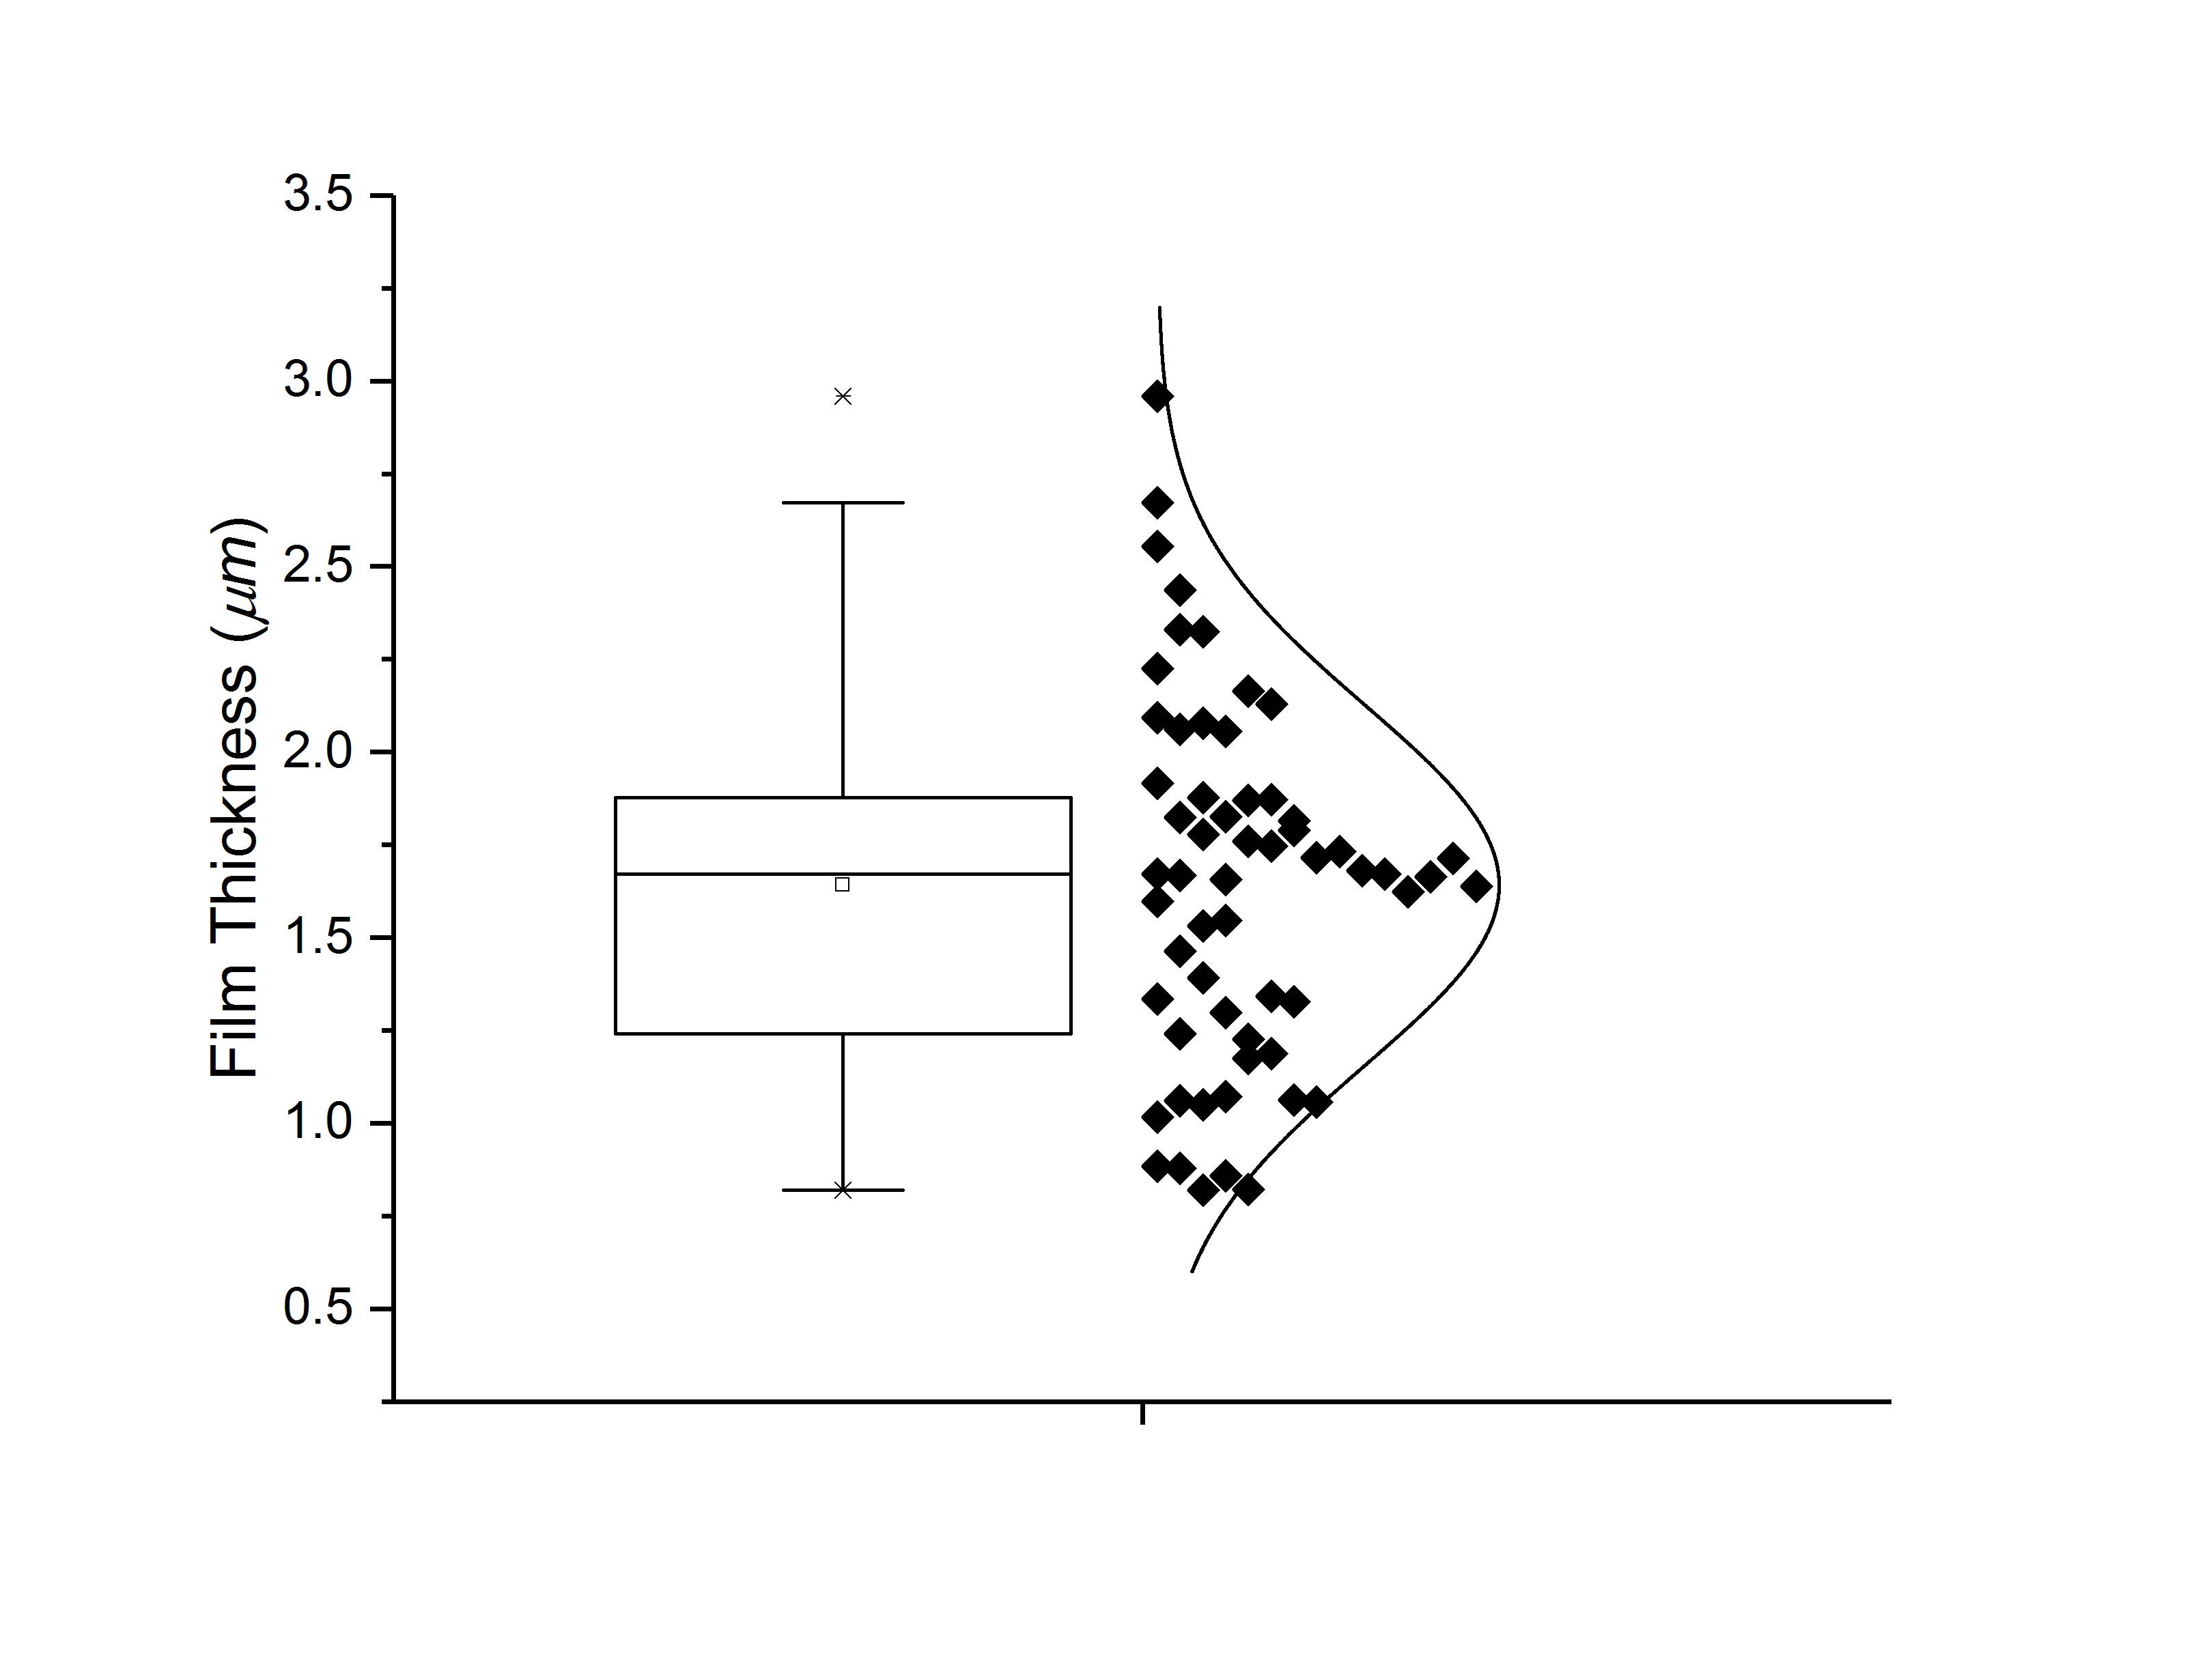
\includegraphics[width=\textwidth]{Film_Thickness.png}
		\caption{}
		\label{fig:Film_Thickness}
	\end{subfigure}
	%Image 2
	\begin{subfigure}[htbp]{0.32\textwidth}
		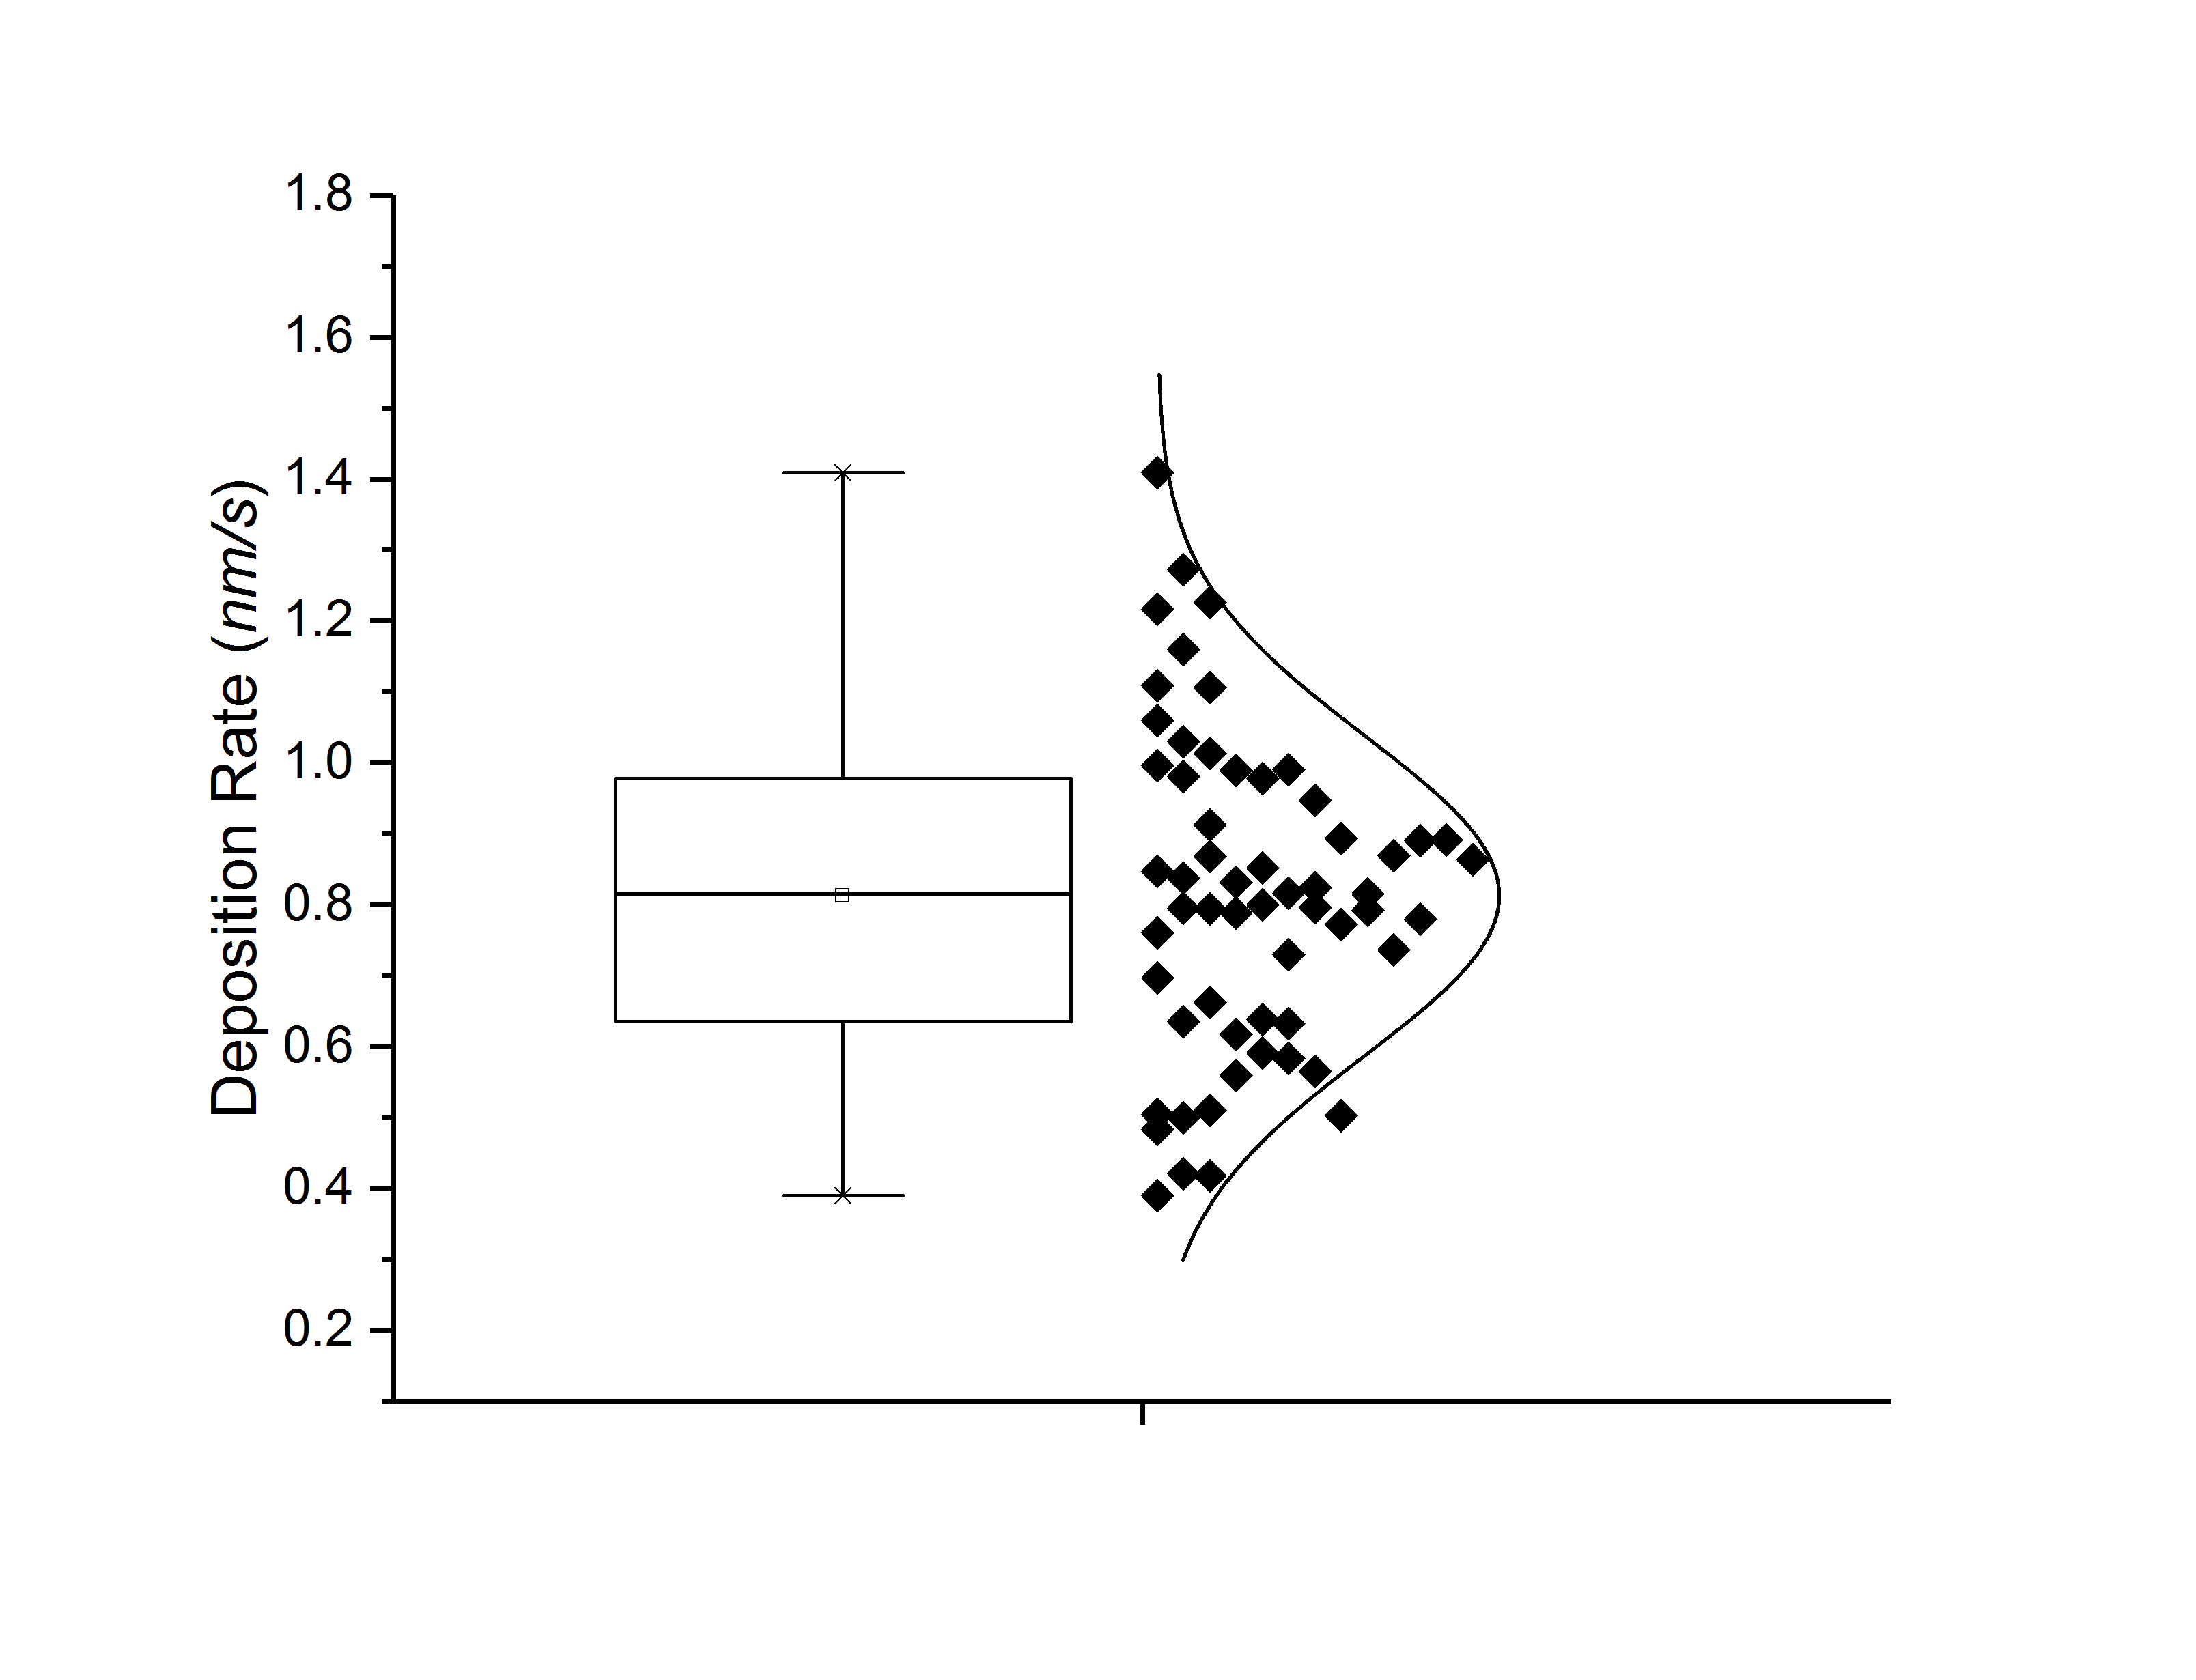
\includegraphics[width=\textwidth]{Deposition_Rate.png}
		\caption{}
		\label{fig:Deposition_Rate}
	\end{subfigure}
	%Image 3
\begin{subfigure}[htbp]{0.32\textwidth}
	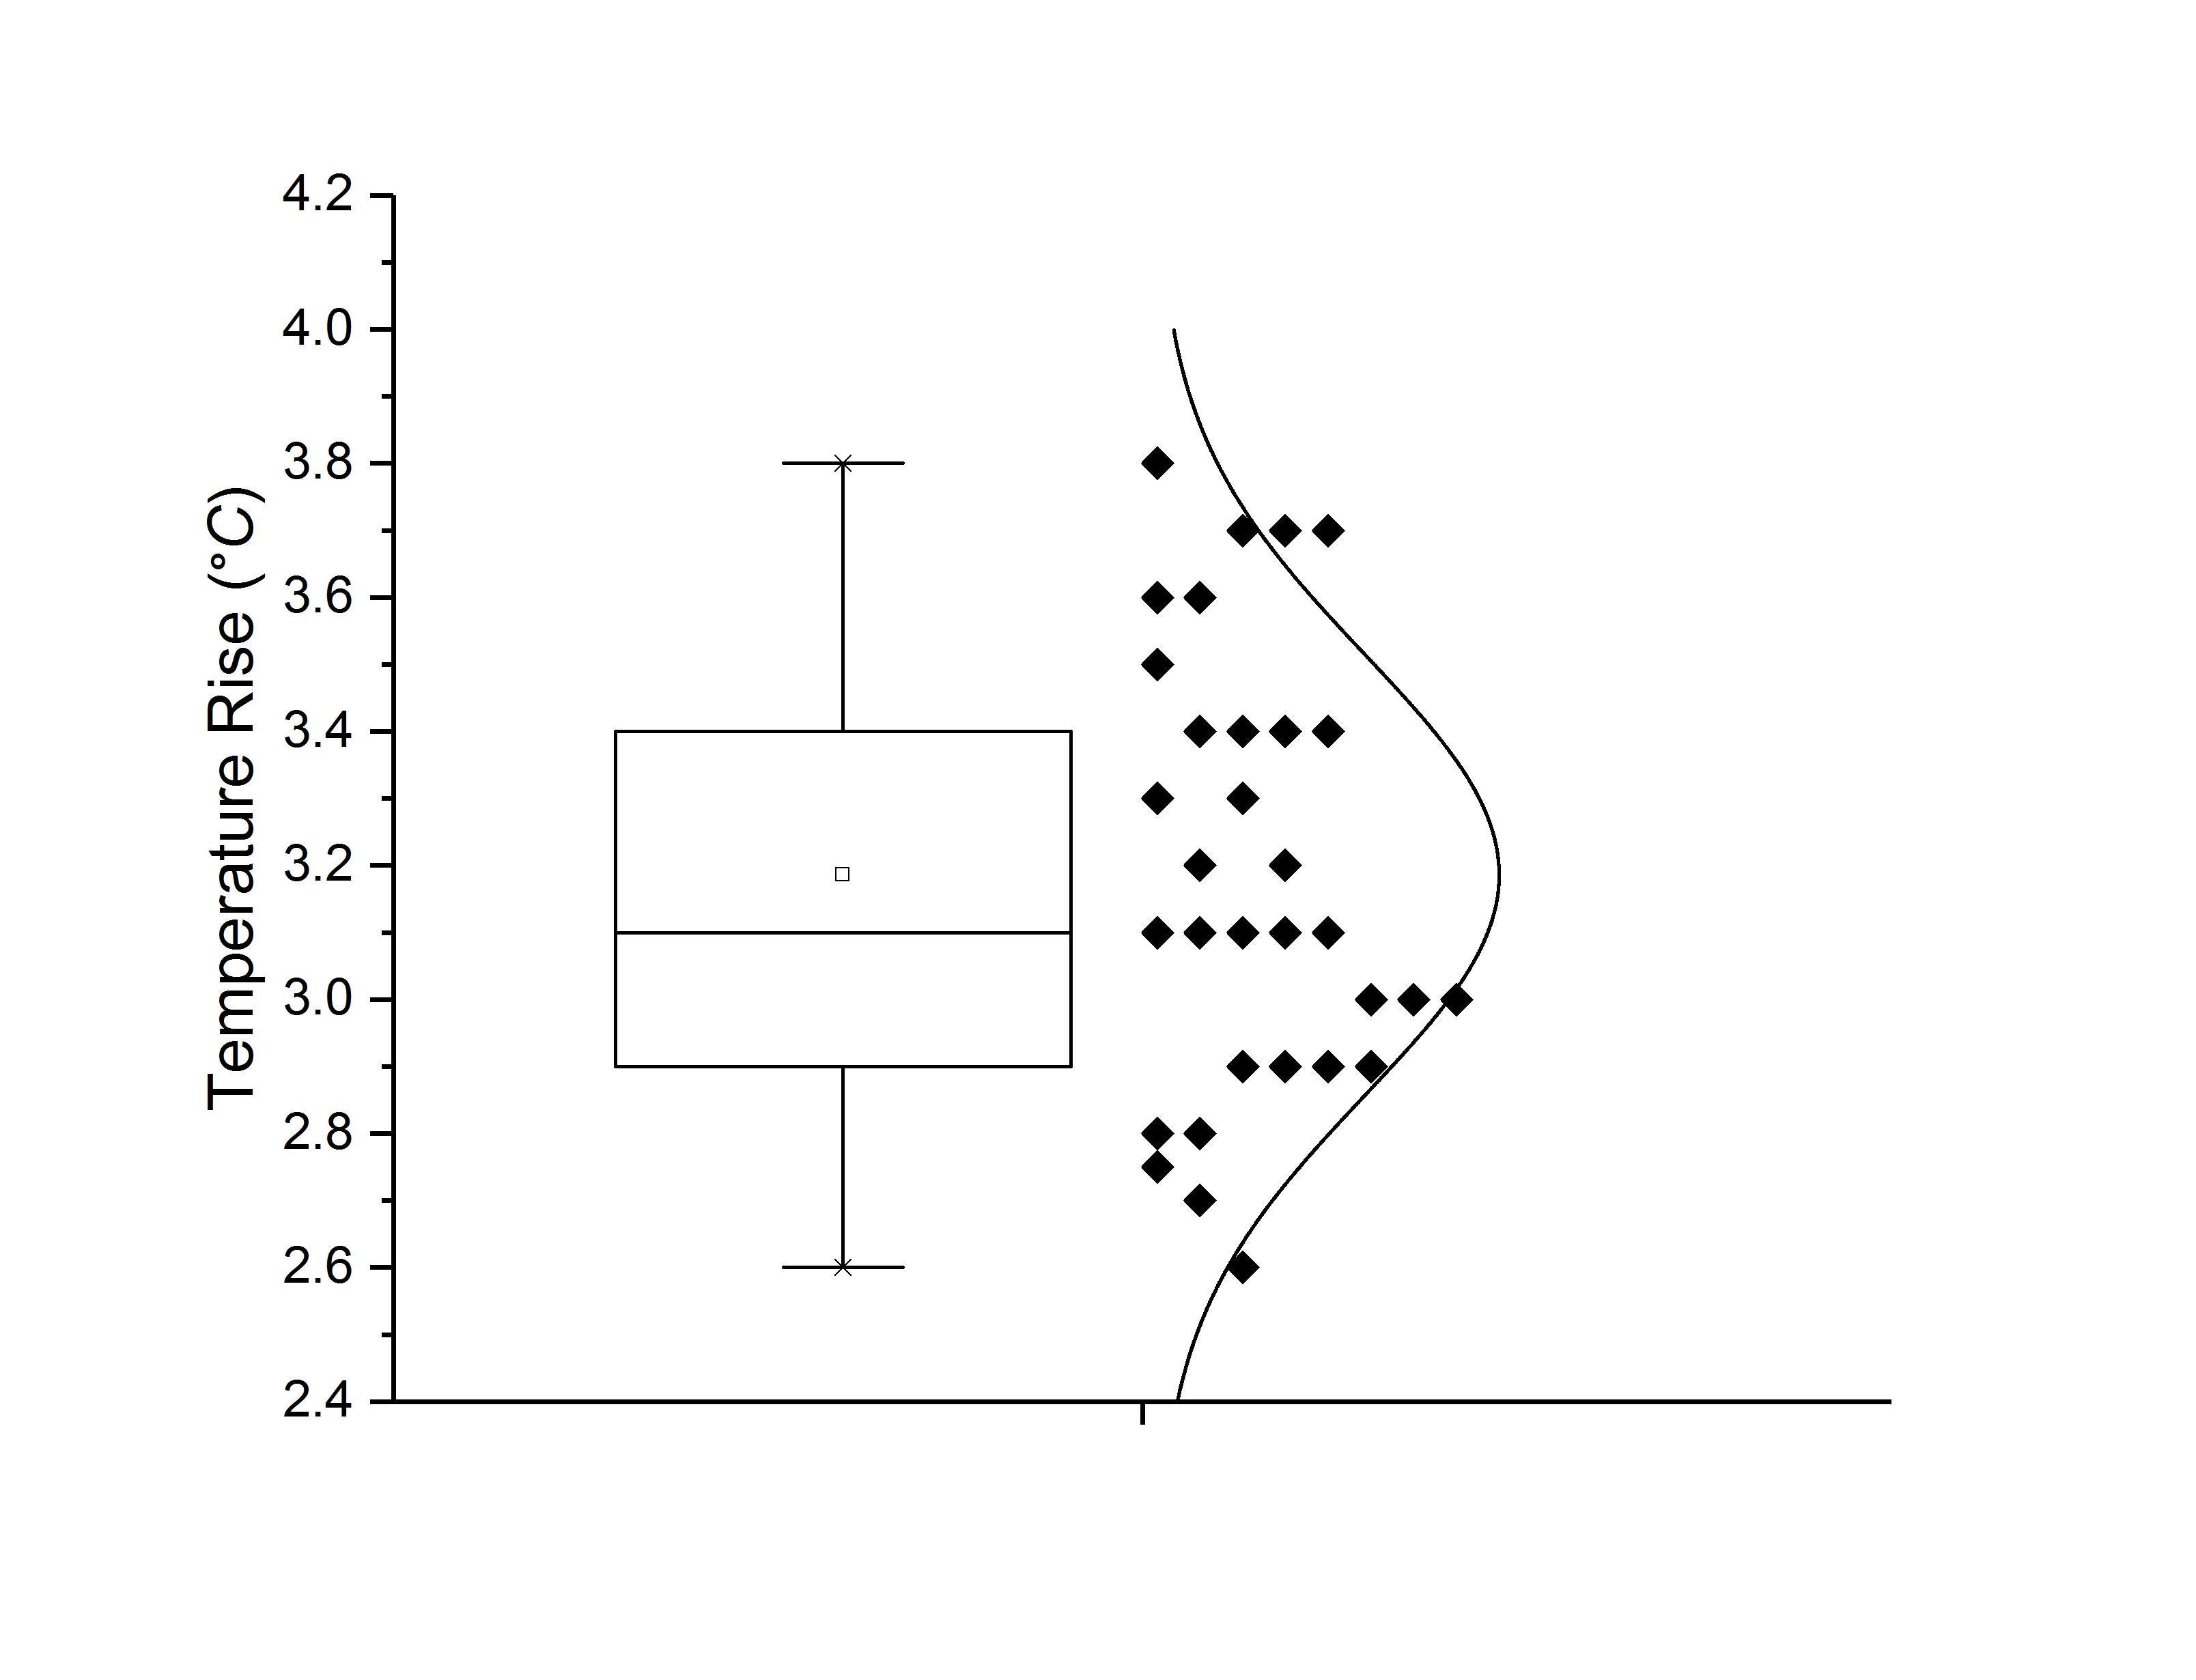
\includegraphics[width=\textwidth]{Temperature_Rise.png}
	\caption{}
	\label{fig:Temperature_Rise}
\end{subfigure}
	\caption{(a) Box and whisker plot of the measured film thicknesses from depositions. (b) Box and whisker plot of the calculated deposition rates achieved. (c) Box and whisker plot of substrate temperature rise.}%global caption
	\label{fig:Film_Thickness_DepRate}
\end{figure}

\acrshort{eds} analysis shows good agreement in the nominal composition for both the bulk and film \MgZnCa, see Table \ref{tab:EDS_Composition}.

\begin{table}[h]
	\centering
	\caption{\acrshort{eds} composition of bulk and film \MgZnCa~ in atomic weight percent.}
	\begin{tabular}{ c c c }
		\toprule
		\acrshort{eds} Analysis & Bulk (at\%)  & Film (at\%)  \\
		\midrule
		Mg & $64.85 \pm 3.18$ & $62.92 \pm 3.24$ \\
		Zn & $29.55 \pm 0.82$ & $31.17 \pm 0.95$ \\
		Ca & $~~ 5.60 \pm 0.17$ & $~~ 5.91 \pm 0.19$ \\ 
		\bottomrule
	\end{tabular}
	\label{tab:EDS_Composition}
\end{table}

\subsection{\acrshort{dsc}}
\subsubsection{Isochronic \acrshort{dsc}}
Isochronic \acrshort{dsc} was performed on the bulk and film \MgZnCa~ to examine the thermal properties. The bulk alloy was relaxed at $120$\degree C for 10 minutes before \acrshort{dsc} measurements to ensure the \Tg~ was clearly visible. The film was not relaxed as unlike the bulk the lost in free volume from relaxation would be significant and make differences between the samples much more difficult to observe [source needed???]. 

The bulk \MgZnCa~ was examined at \acrfullpl{ht} of 5, 10, 15, 20, 30, 40, 60, 80, and 100 $K/min$ to observe changes in the \Tg~ and the \Tx s with \gls{ht}. As expected greater \gls{ht} resulted in greater signal strength, exothermic peaks shifting to higher start temperatures, and an increase in thermal lag resulting in later exothermic finish temperatures and curve convolution. With this convolution the \Tg~ and \Tx $_{1}$  remained clearly visible for all \glspl{ht}, but \Tx $_{2,4,5}$ were only visible at low \glspl{ht}, and \Tx $_{3}$ was not clear at any \gls{ht}, see Figure \ref{fig:DSC_vHeatingRate_Bulk}.

The film was examined at \glspl{ht} of 15, 20, 30, 40, 60, 80, and 100 $K/min$. The lower \glspl{ht} of 5 and 10 $k/min$ were not utilised owing to the lower film signal compared to the bulk. The reduced signal was likely from the low mass of the film, about $\frac{1}{10}$ that of the bulk. The film showed the expected variable relationships with increasing \gls{ht} as observed in the bulk. The signal intensity increased at a compatible rate to bulk up until \glspl{ht} of 80 and 100 $k/min$. These final two \glspl{ht} showed great increases in the signal intensity. The exothermic peaks all convoluted together making many of the thermodynamic events difficult to observer at all \glspl{ht}. It also appeared that all exothermic events shifted to lower temperatures as compared to the bulk. The film \Tg~ and \Tx $_{1}$s were less defined than for the bulk, but could still be identified for all \glspl{ht}. For all \glspl{ht} the \Tx $_{2-5}$ onsets could not be easily identified, see Figure \ref{fig:DSC_vHeatingRate_Film}.

%single image
\begin{figure}[b]
	\centering
	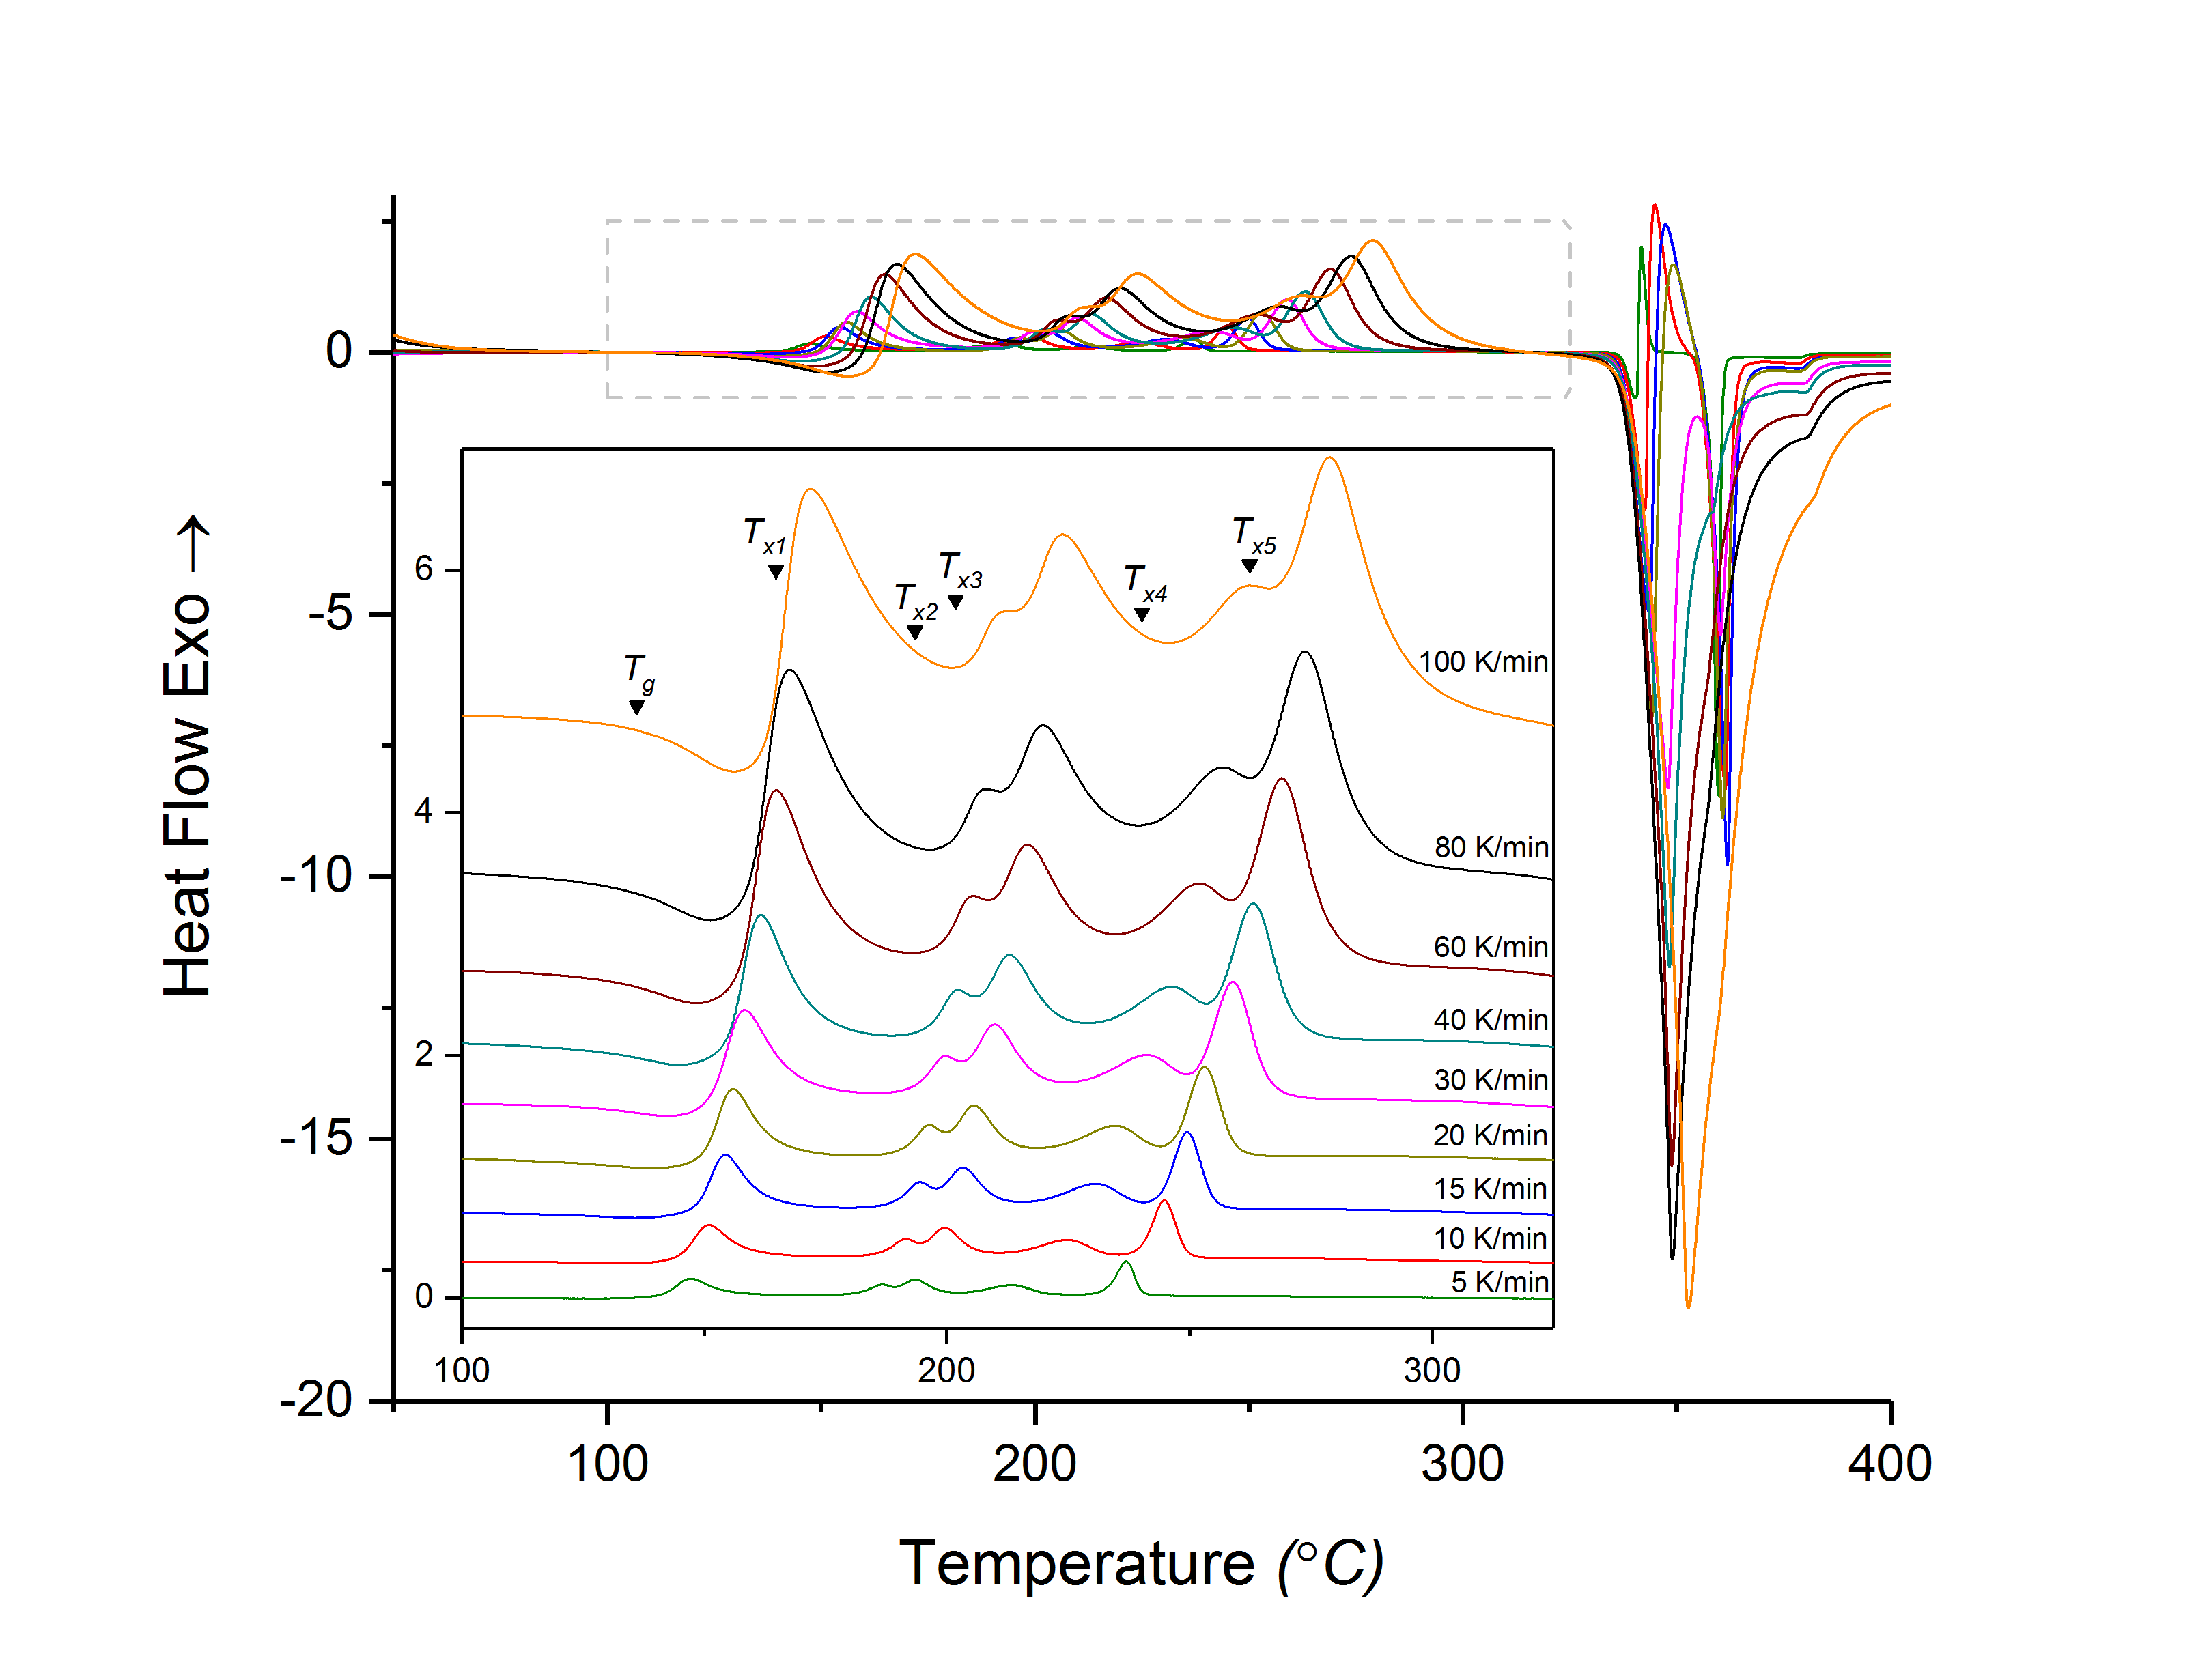
\includegraphics[width=0.65\textwidth]{DSC_Fragility_Bulk.png}
	\caption{Bulk \MgZnCa~ relaxed at 120 \degree C for 10 minutes and heated at various \acrfullpl{ht} from $5$ to $100 K/min$. The insert stacks the \gls{dsc} curves and labels the \Tg~ and \Tx s of the \gls{ht} $=100 K/min$ curve.}%global caption
	\label{fig:DSC_vHeatingRate_Bulk}
\end{figure}

%single image
\begin{figure}[b]
	\centering
	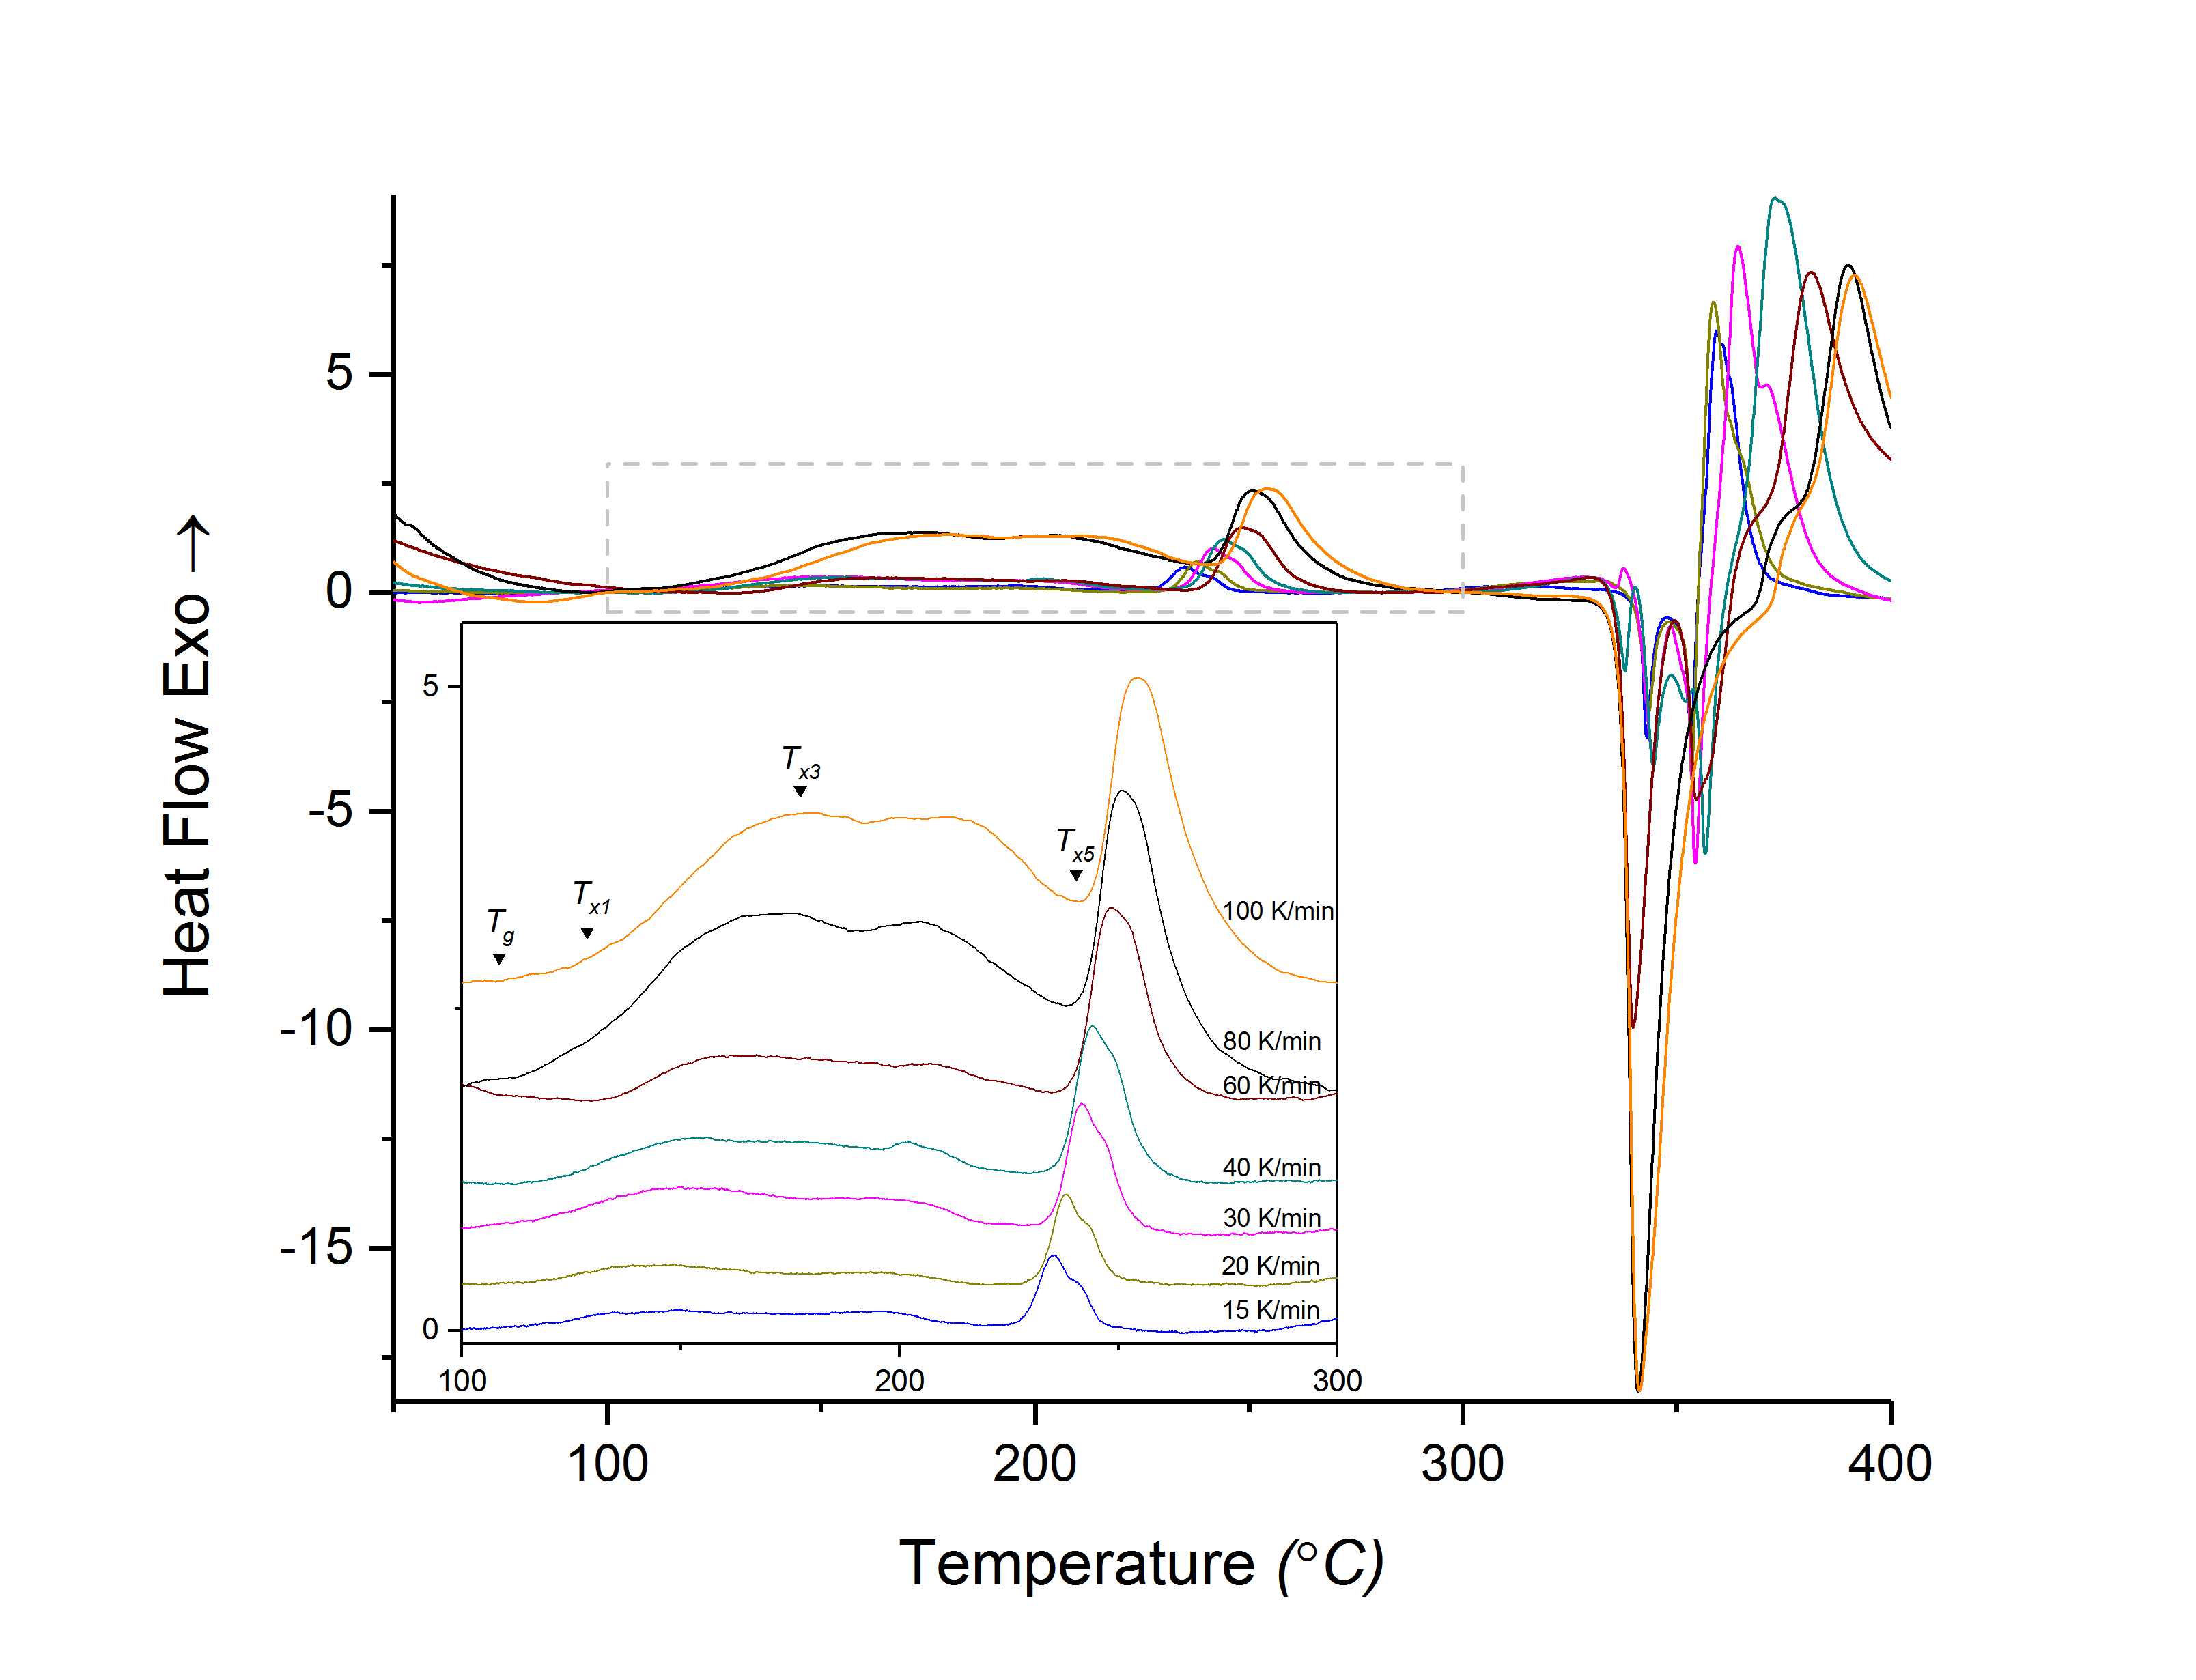
\includegraphics[width=0.65\textwidth]{DSC_Fragility_Film.png}
	\caption{Unrelaxed film \MgZnCa~ heated at various \acrfullpl{ht}  from $15$ to $100 K/min$. The insert stacks the \gls{dsc} curves and labels the \Tg~ and \Tx s of the \gls{ht} $=100 K/min$ curve.}%global caption
	\label{fig:DSC_vHeatingRate_Film}
\end{figure}

\subsubsection{Fragility}

Using the isochronic \acrshort{dsc} data the \gls{m} of the \MgZnCa~ system could be established for both the bulk and film. Numerical solutions where used to fit the \acrshort{dsc} variant of the \gls{vft} relationship for \gls{ht} \cite{Busch1998}.

\begin{equation}
	\beta^{-1} = \tau_{0}~ e^{(\frac{D^{*}T_{0}}{T_{g}-T_{0}})}
	\label{equ:VFT}
\end{equation}

Where $\tau_{0}$ is a pre-exponential factor, $D^{*}$ is the liquid \acrlong{m} parameter, and $T_{0}$ is the \gls{vft} temperature where the barrier to flow becomes infinite.

The \gls{m} could then be calculated from Equation \ref{equ:dStar} \cite{Angell2002, Wei2014}.

\begin{equation}
	D^{*}=590/(m-16)
	\label{equ:dStar}
\end{equation}

Using these two equations for the bulk it was found $\beta^{-1} = 1.338E - 16e^{5274 (\frac{1}{T-T_{0}})}$ with an Adj. $R^{2}=0.972$. This gave a $D^{*}=20.4$, and a \gls{m}$=44.9$. The film was fitted to $\beta^{-1} = 5.921E - 11e^{2766 (\frac{1}{T-T_{0}})}$ with a lower confidence of Adj. $R^{2}=0.861$, likely owing to the reduced number of data points. This gave a $D^{*}=10.0$, and \gls{m}$=75.0$, see Figure \ref{fig:Fragility_BulkFilm_mValue}.

%single image
\begin{figure}[b]
	\centering
	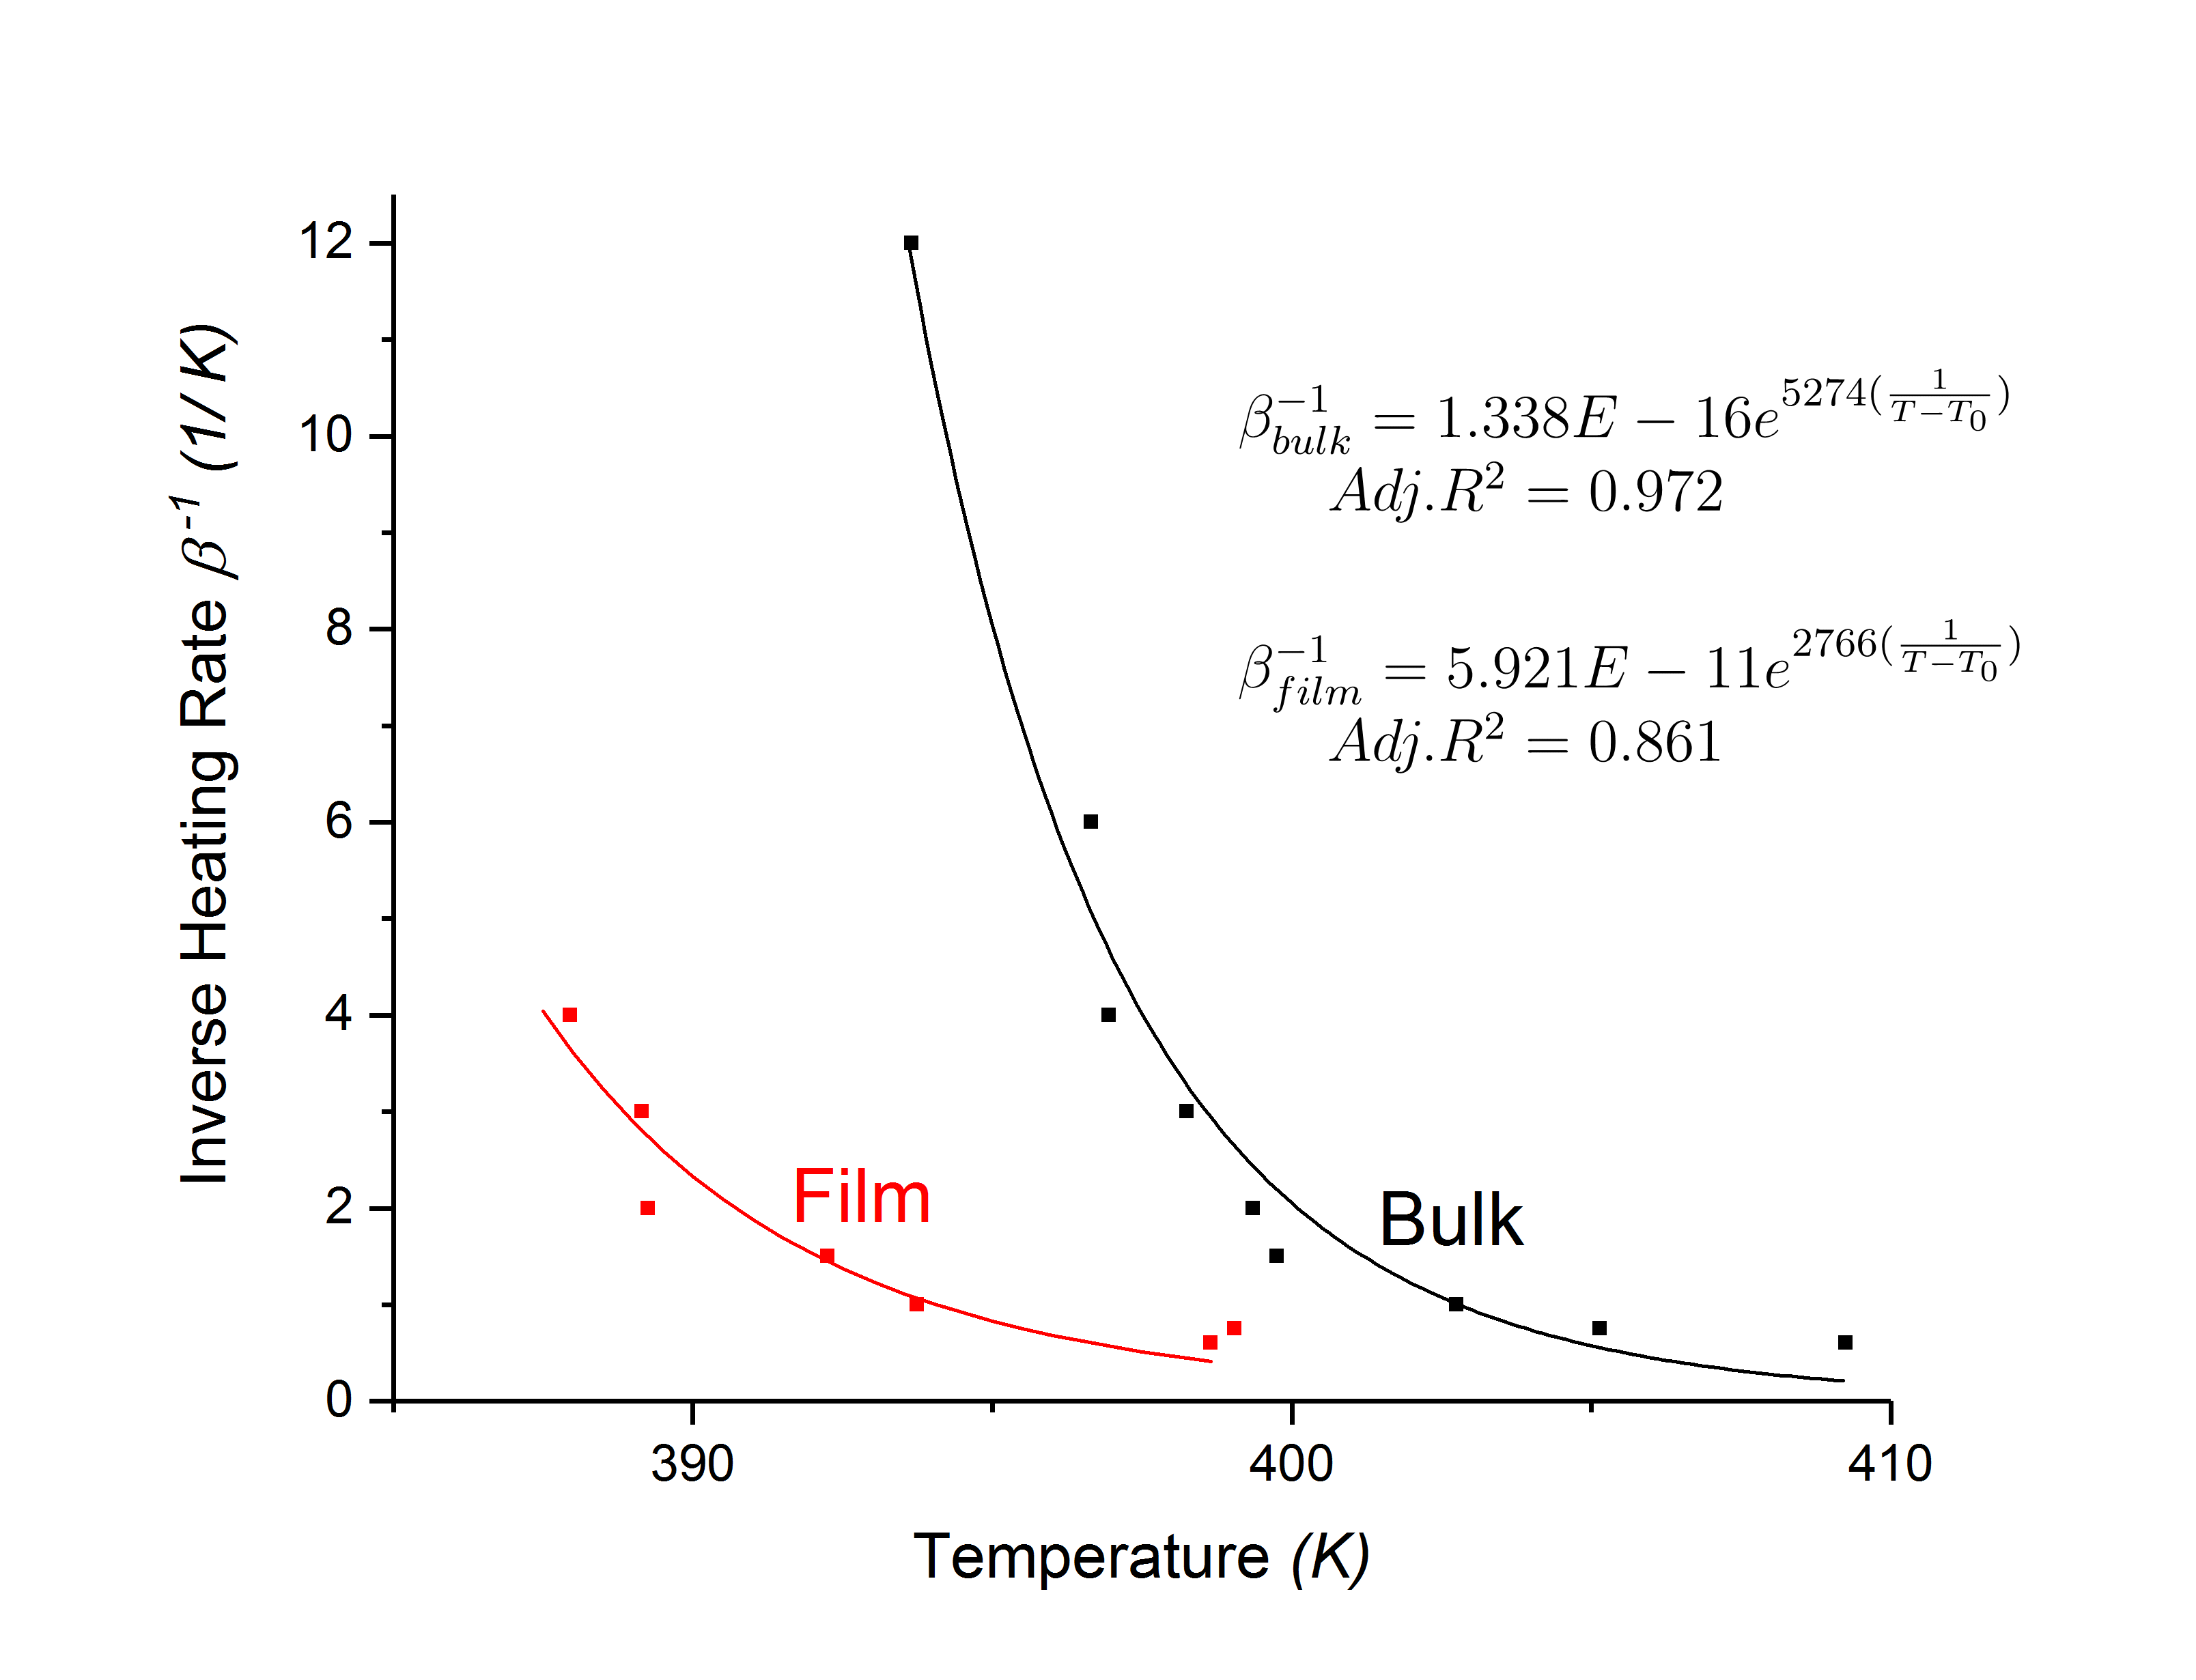
\includegraphics[width=0.95\textwidth]{Bulk_Film_Fragility.png}
	\caption{Fitted \acrfull{m} for the \MgZnCa~ system obtained from the \Tg~ of \acrshort{dsc} at various \acrfullpl{ht} for the bulk and film.}
	\label{fig:Fragility_BulkFilm_mValue}
\end{figure}

\subsection{\acrshort{dsc} deconvolution}

\subsubsection{Onset determination}

Numerical 
solutions were used to deconvolute the isochronic \acrshort{dsc} data so the various \Tx~ onsets could be accurately determined. This numerical fitting utilised a summation of skewed Gaussian curves to fit a target curve corresponding to the original data; as is a common method \cite{Ashour2010, Yamamoto2007, Spink2008, Spink2015, Schaffer2005}. This fitting summation takes the form of Equation \ref{equ:GaussianSummation} \todo{this is non-skewed form. It is a place holder}.

\begin{equation}
	f(x) = \sum_{n=i}^{n} h_{i}~ e^-{\bigg(\frac{(x-T_{i})^2}{(2c_{j})^2}\bigg)}
	\label{equ:GaussianSummation}
\end{equation}

Where $h$ is the magnitude of the enthalpy peak, $T$ is the temperature at the enthalpy peak centre, and $c$ is the Gaussian RMS width.

The final deconverged solutions of this fitting for both the bulk and film are shown in Figures \ref{fig:DSC_Bulk_Decon} and \ref{fig:DSC_Film_Decon} respectively. These results are tabulated in Table \ref{tab:BulkOnsets} for the bulk and Table \ref{tab:FilmOnsets} for the film. Tables \ref{tab:BulkOnsets} and \ref{tab:FilmOnsets} are also plotted together in Figure \ref{fig:DSC_Onsets_BulkFilm} with the bulk shown in black and the film in red. Note \Tg~ and \Tx$_{1}$ are obtained from the original raw data, not the deconvolution.

It is worth noting the deconvolution fitted 5 crystallisation events for the bulk \MgZnCa, but only 3 events for the film. This occured because the bulk had 5 well defined events, where as the film was largely convoluted together. Thus unique solutions could not be obtained for the lesser \Tx$_{2}$ and \Tx$_{4}$ events of the film. 

%MultiFigure
\begin{figure}[b]
	\centering
	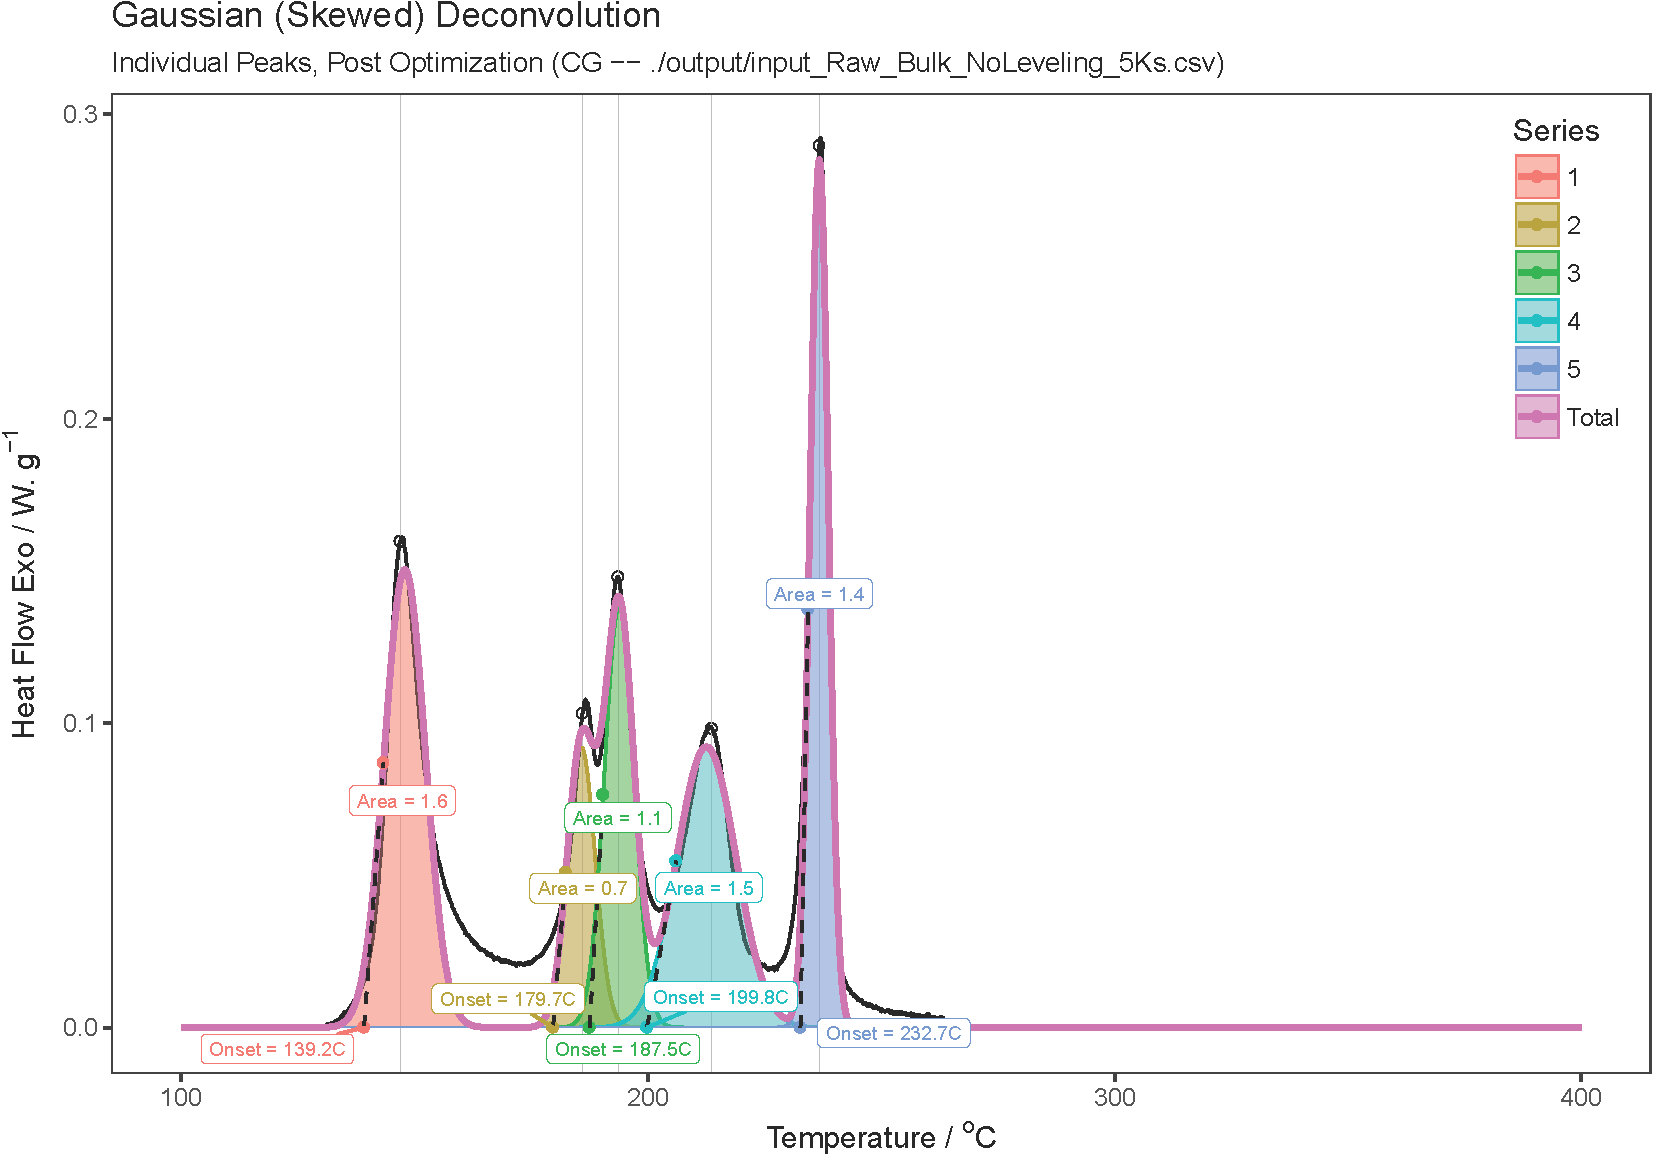
\includegraphics[width=.3\textwidth]{input_Raw_Bulk_NoLeveling_5Ks_result_A5lsc.png}\quad
	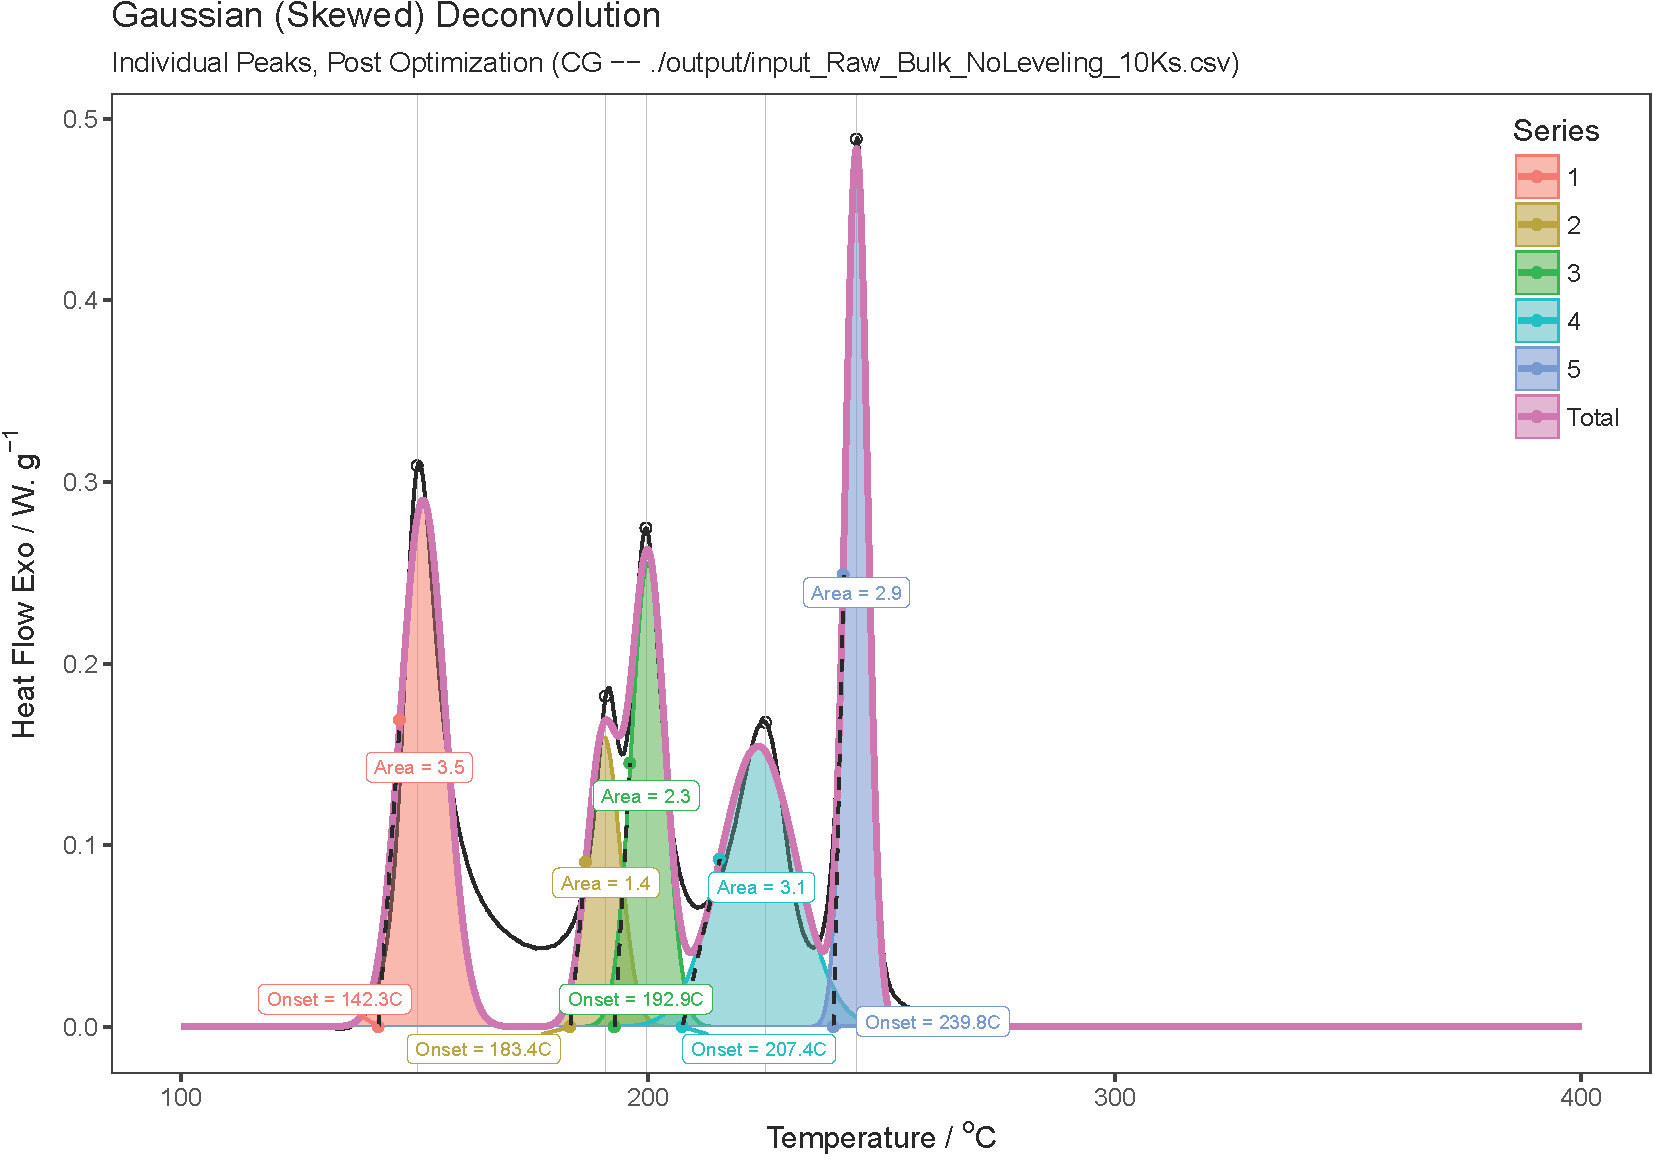
\includegraphics[width=.3\textwidth]{input_Raw_Bulk_NoLeveling_10Ks_result_A5lsc.png}\quad
	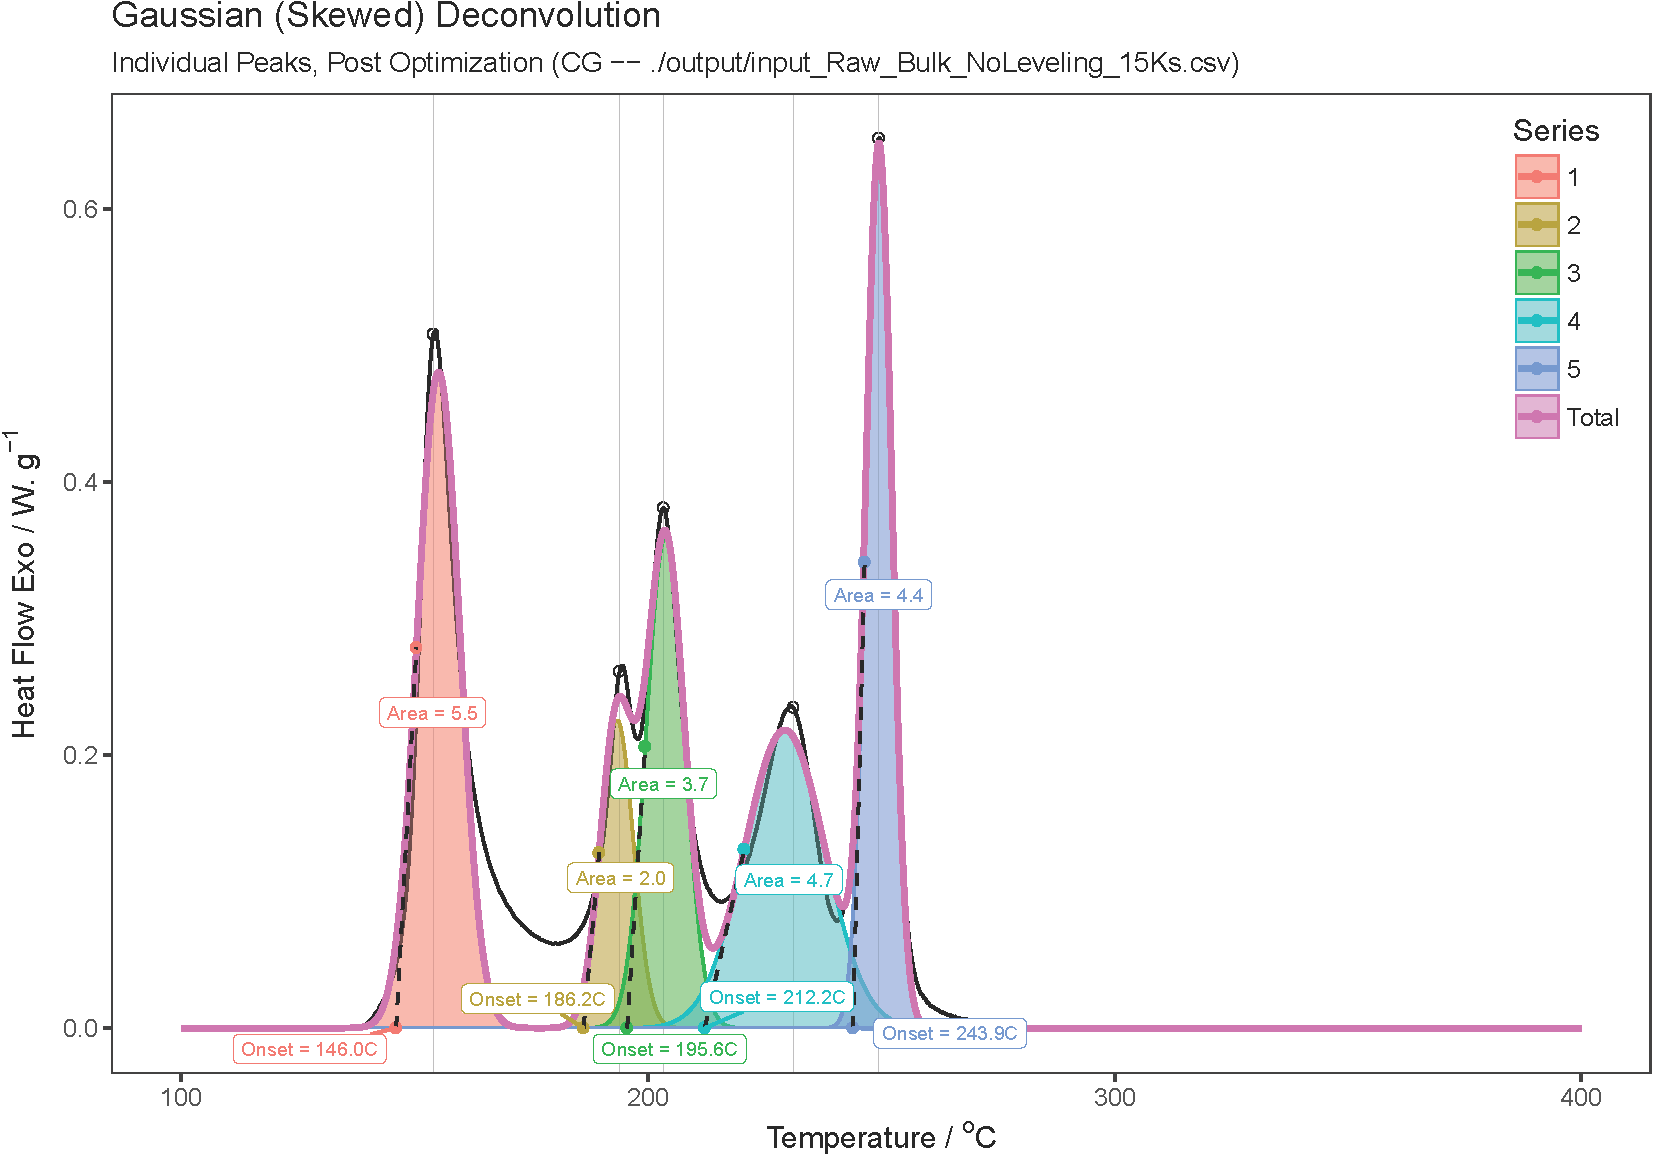
\includegraphics[width=.3\textwidth]{input_Raw_Bulk_NoLeveling_15Ks_result_A5lsc.png}
	\medskip
	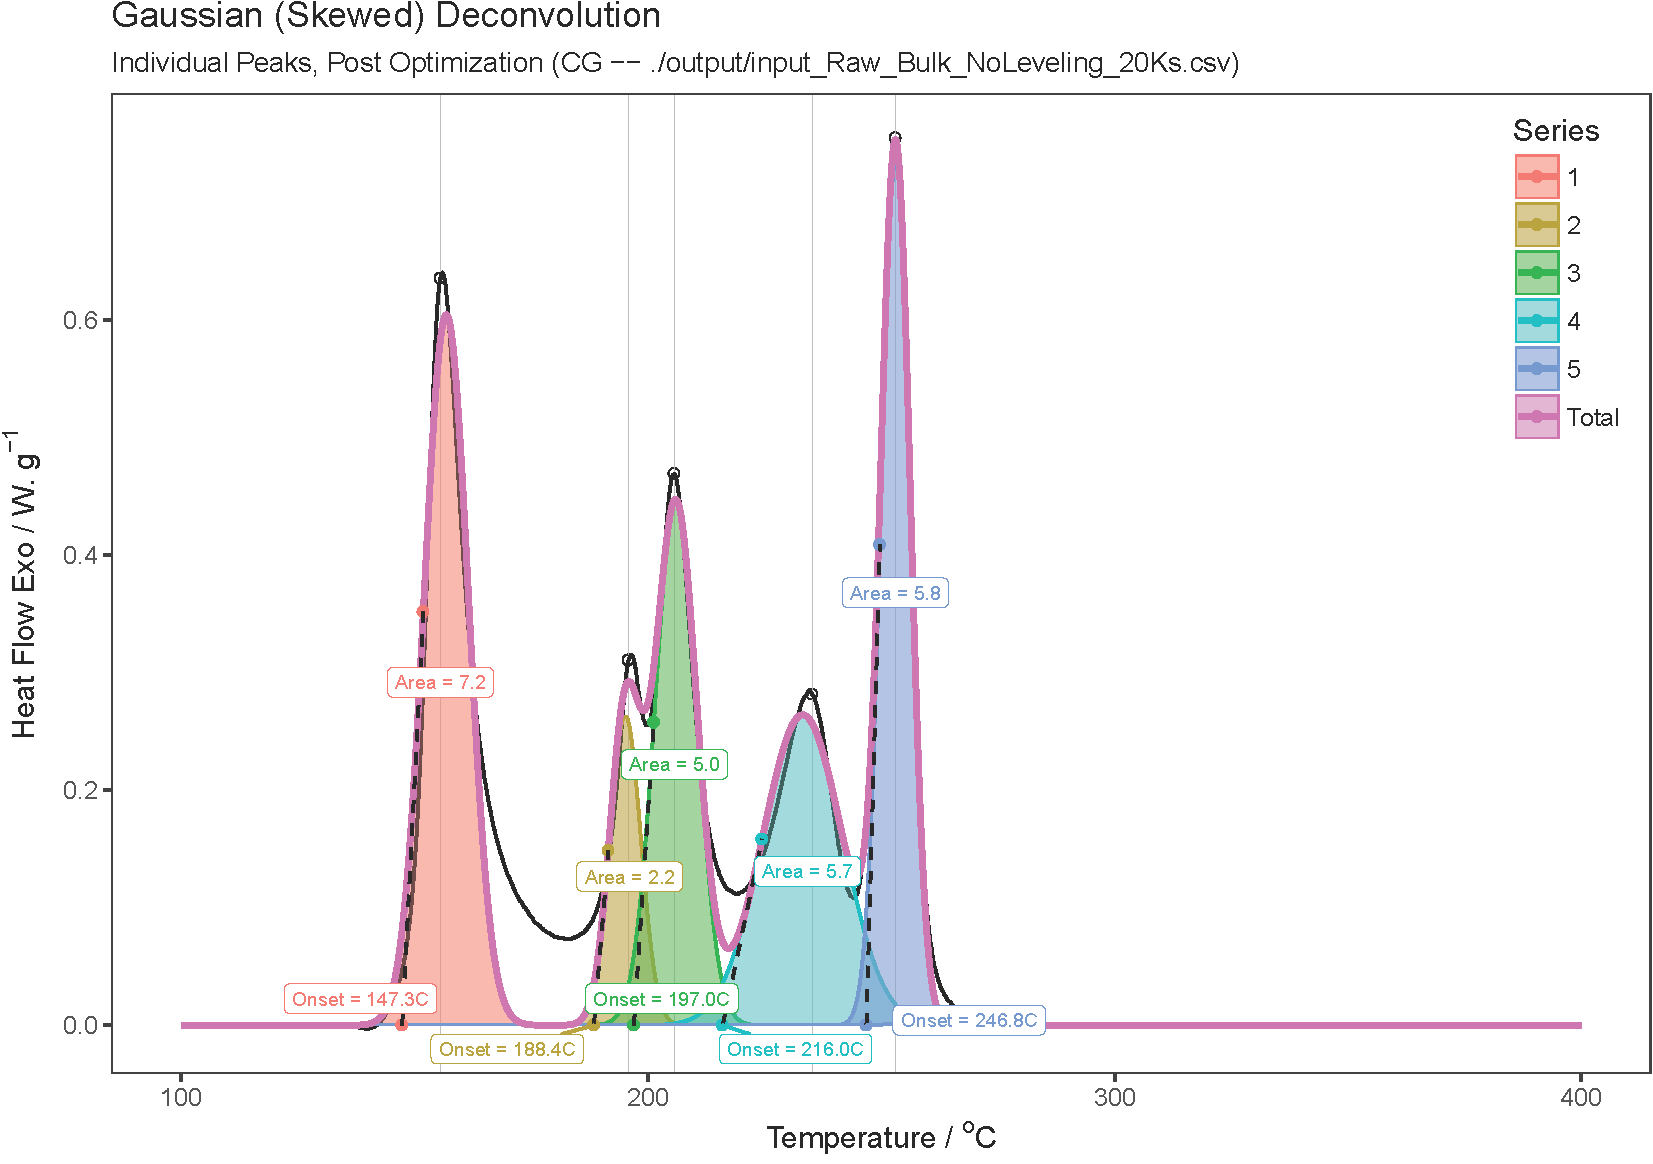
\includegraphics[width=.3\textwidth]{input_Raw_Bulk_NoLeveling_20Ks_result_A5lsc.png}\quad
	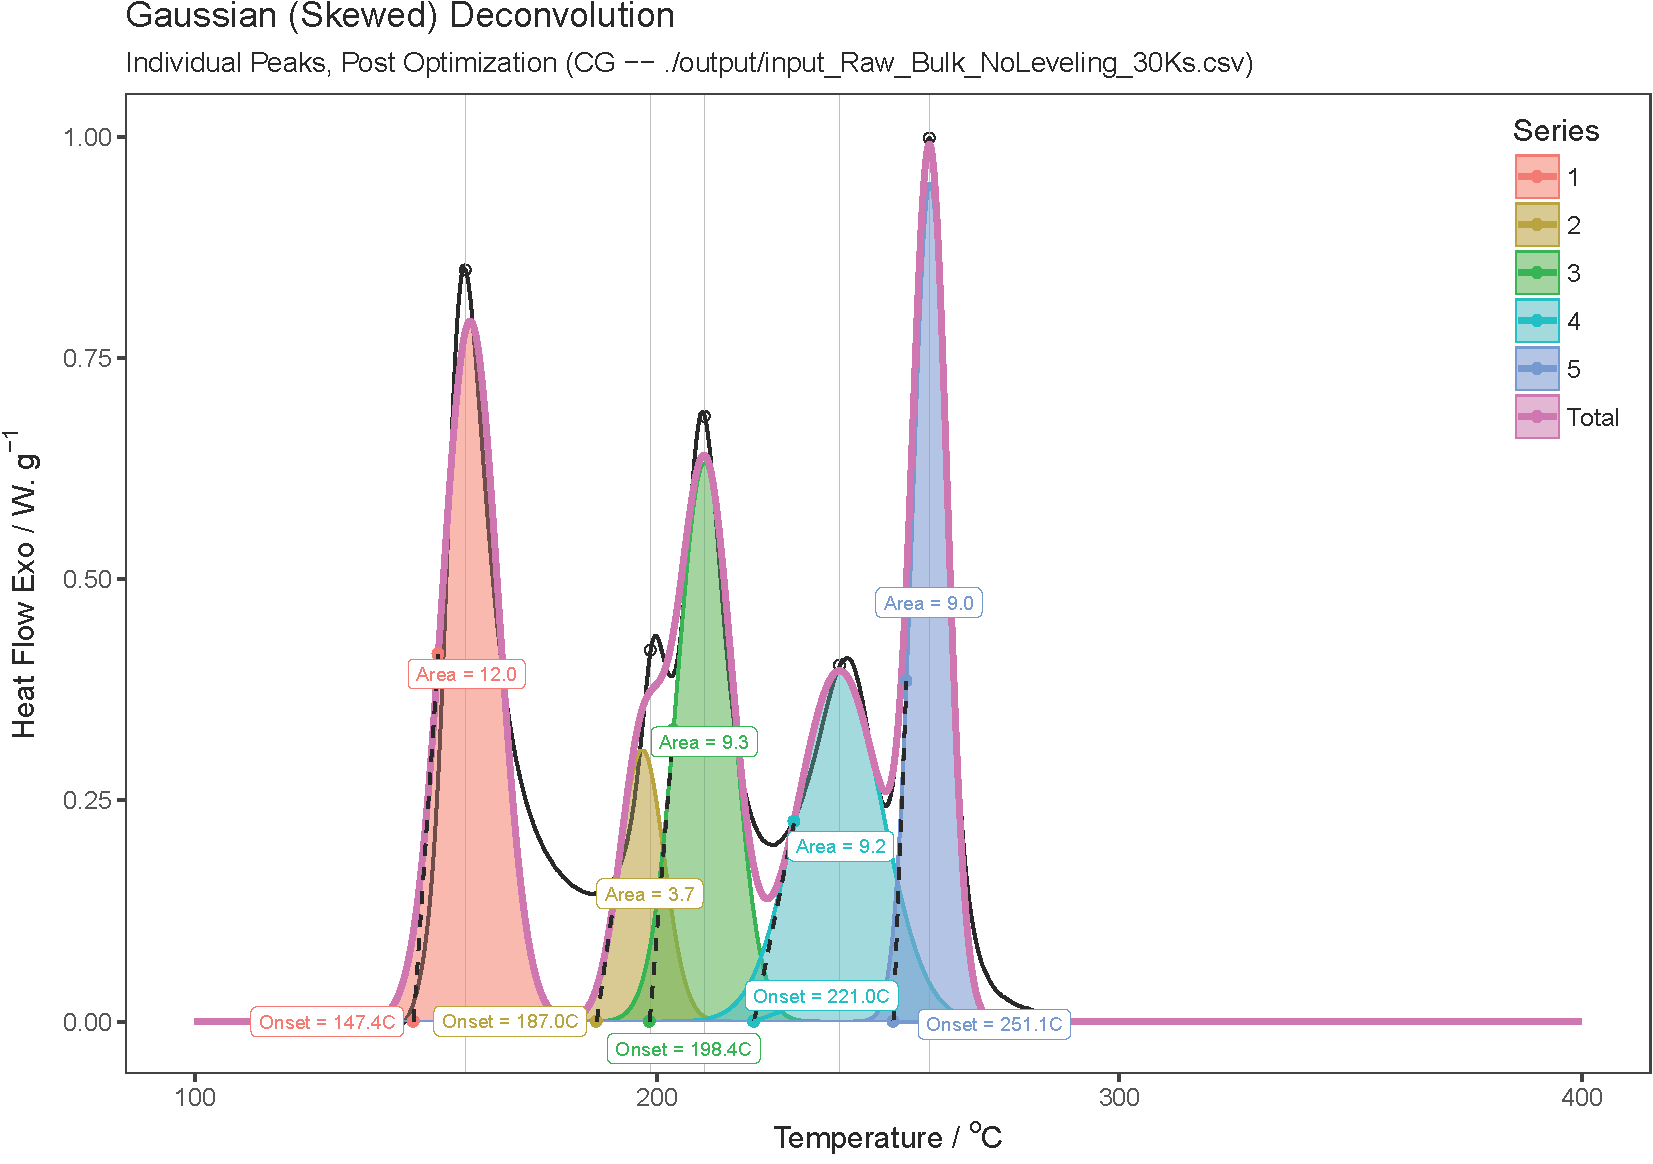
\includegraphics[width=.3\textwidth]{input_Raw_Bulk_NoLeveling_30Ks_result_A5lsc.png}\quad
	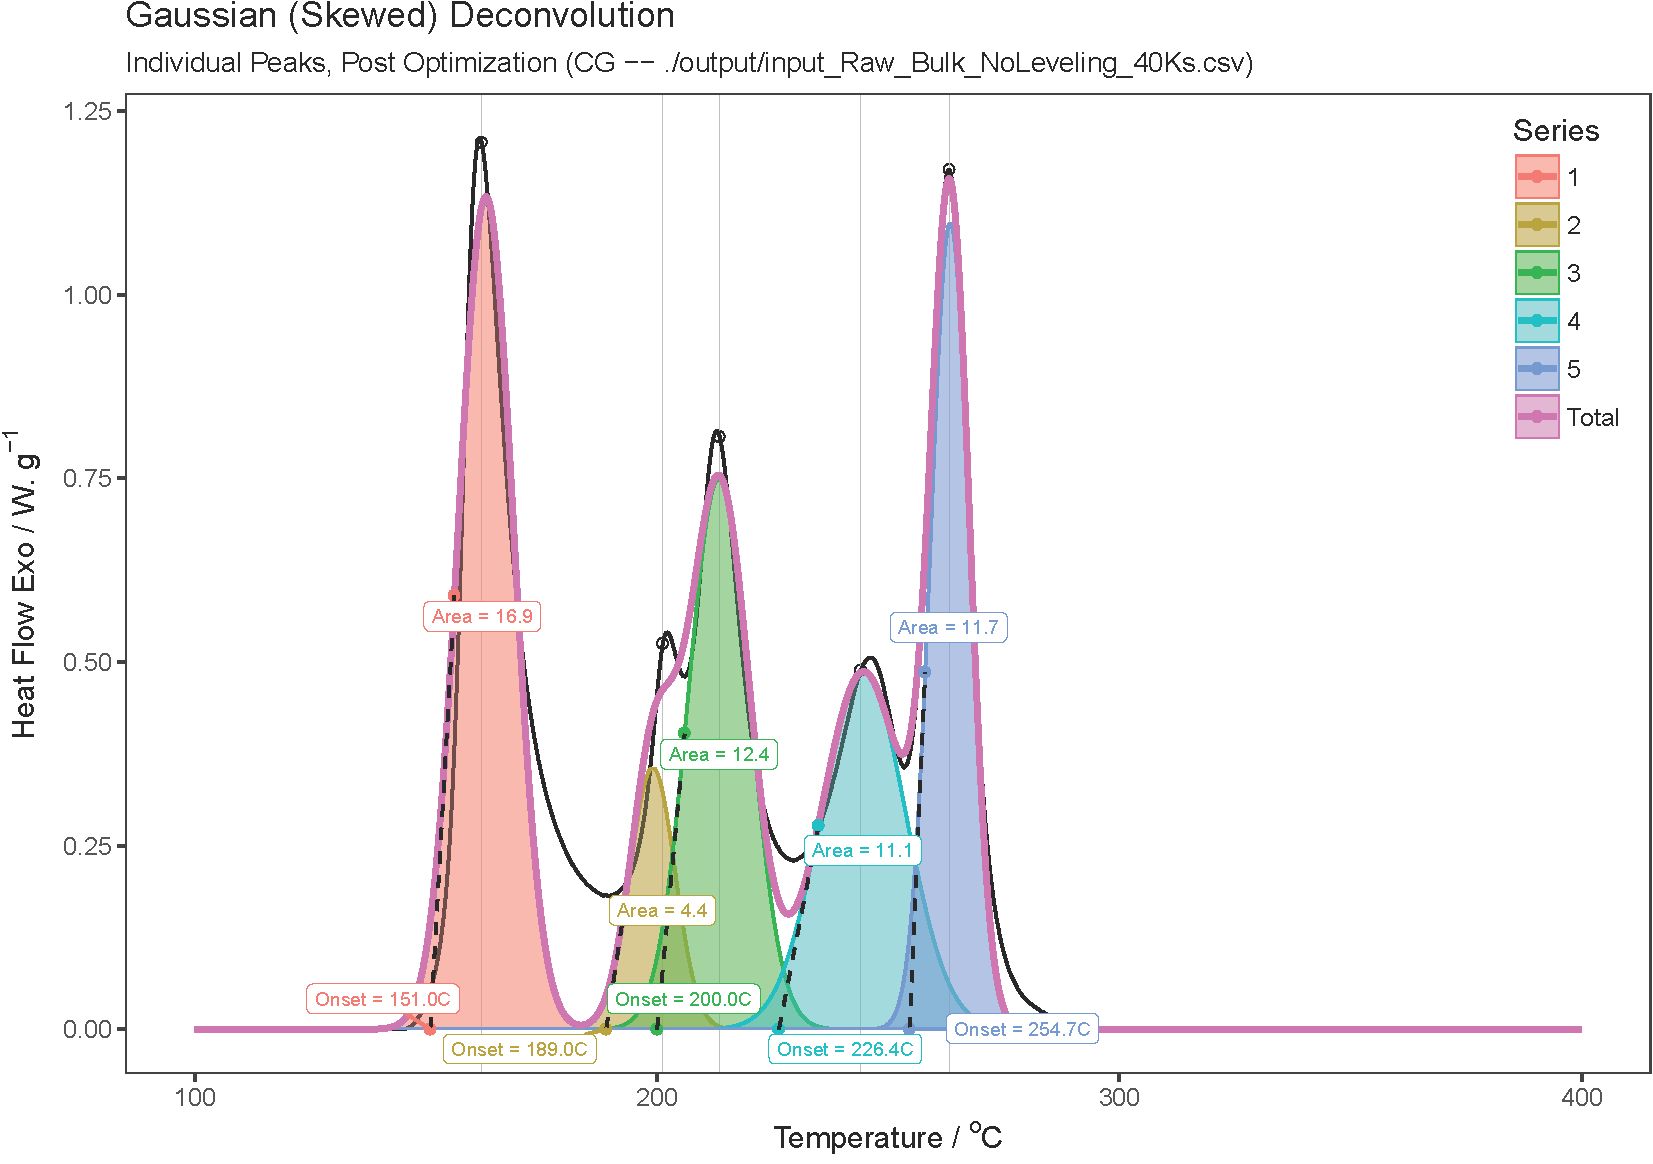
\includegraphics[width=.3\textwidth]{input_Raw_Bulk_NoLeveling_40Ks_result_A5lsc.png}
	\medskip
	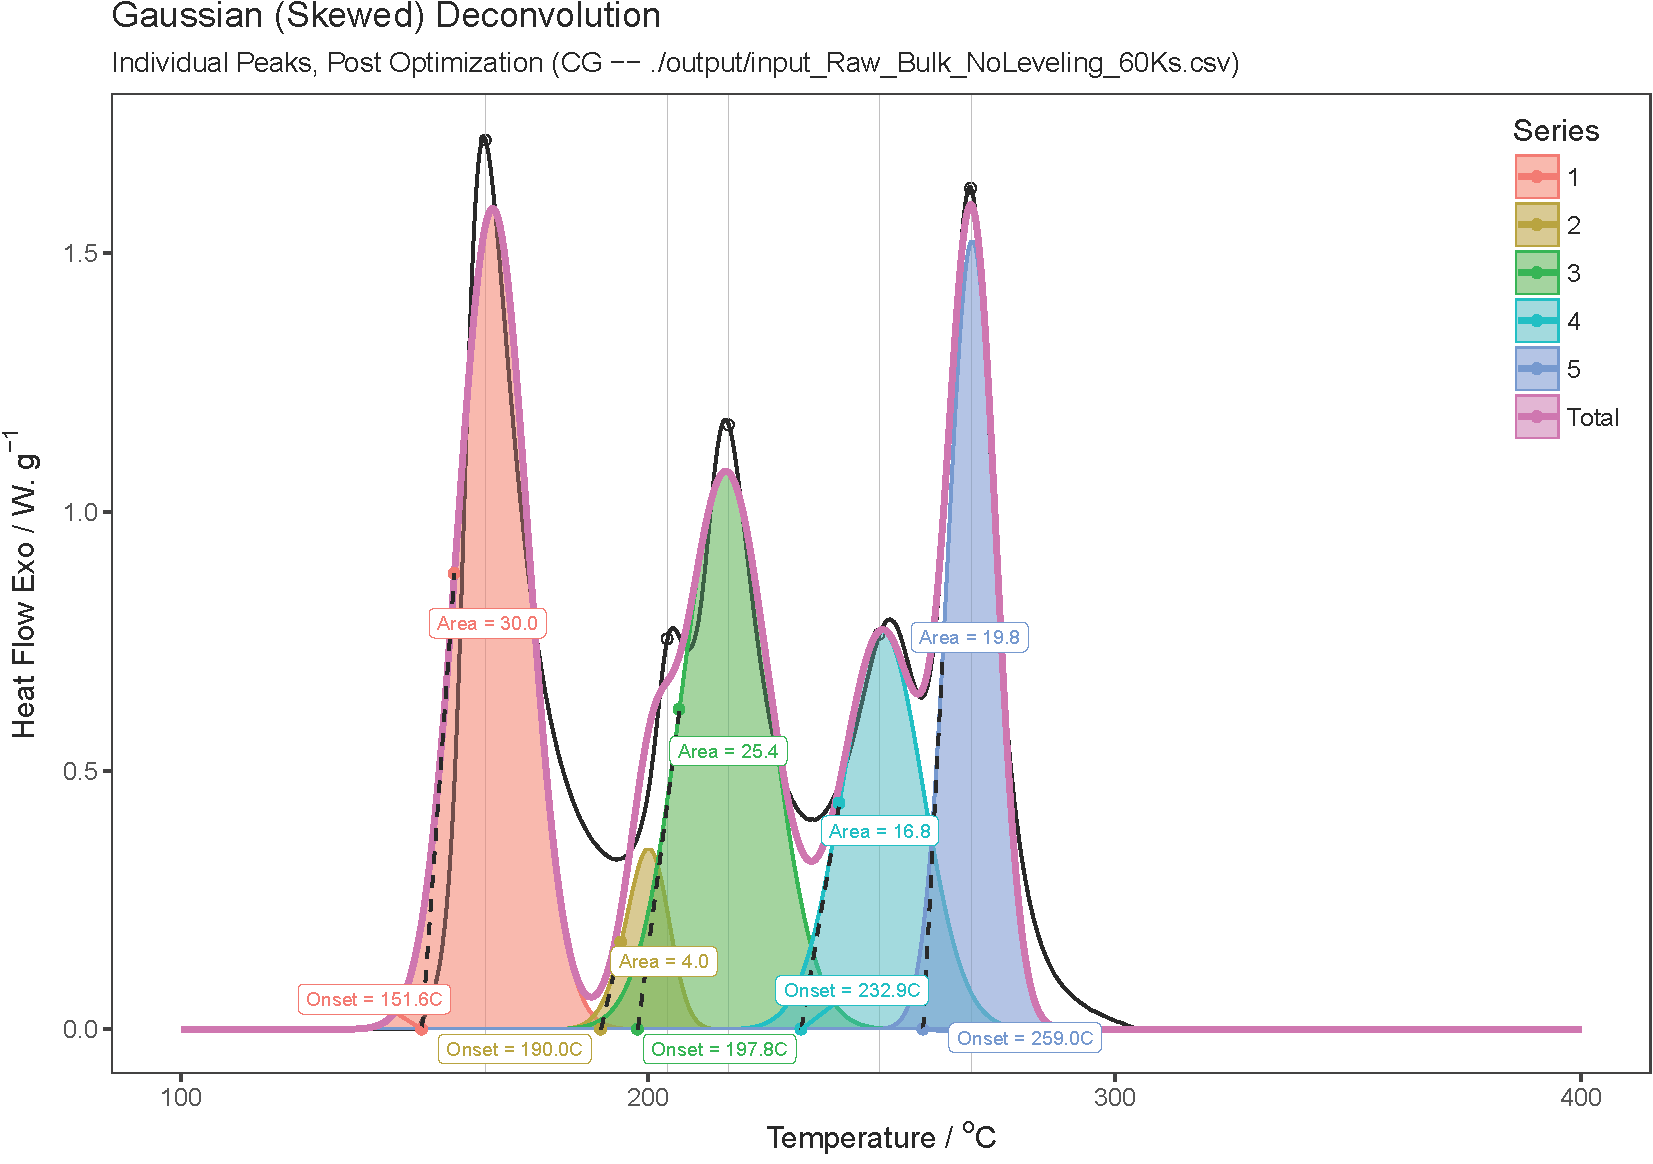
\includegraphics[width=.3\textwidth]{input_Raw_Bulk_NoLeveling_60Ks_result_A5lsc.png}\quad
	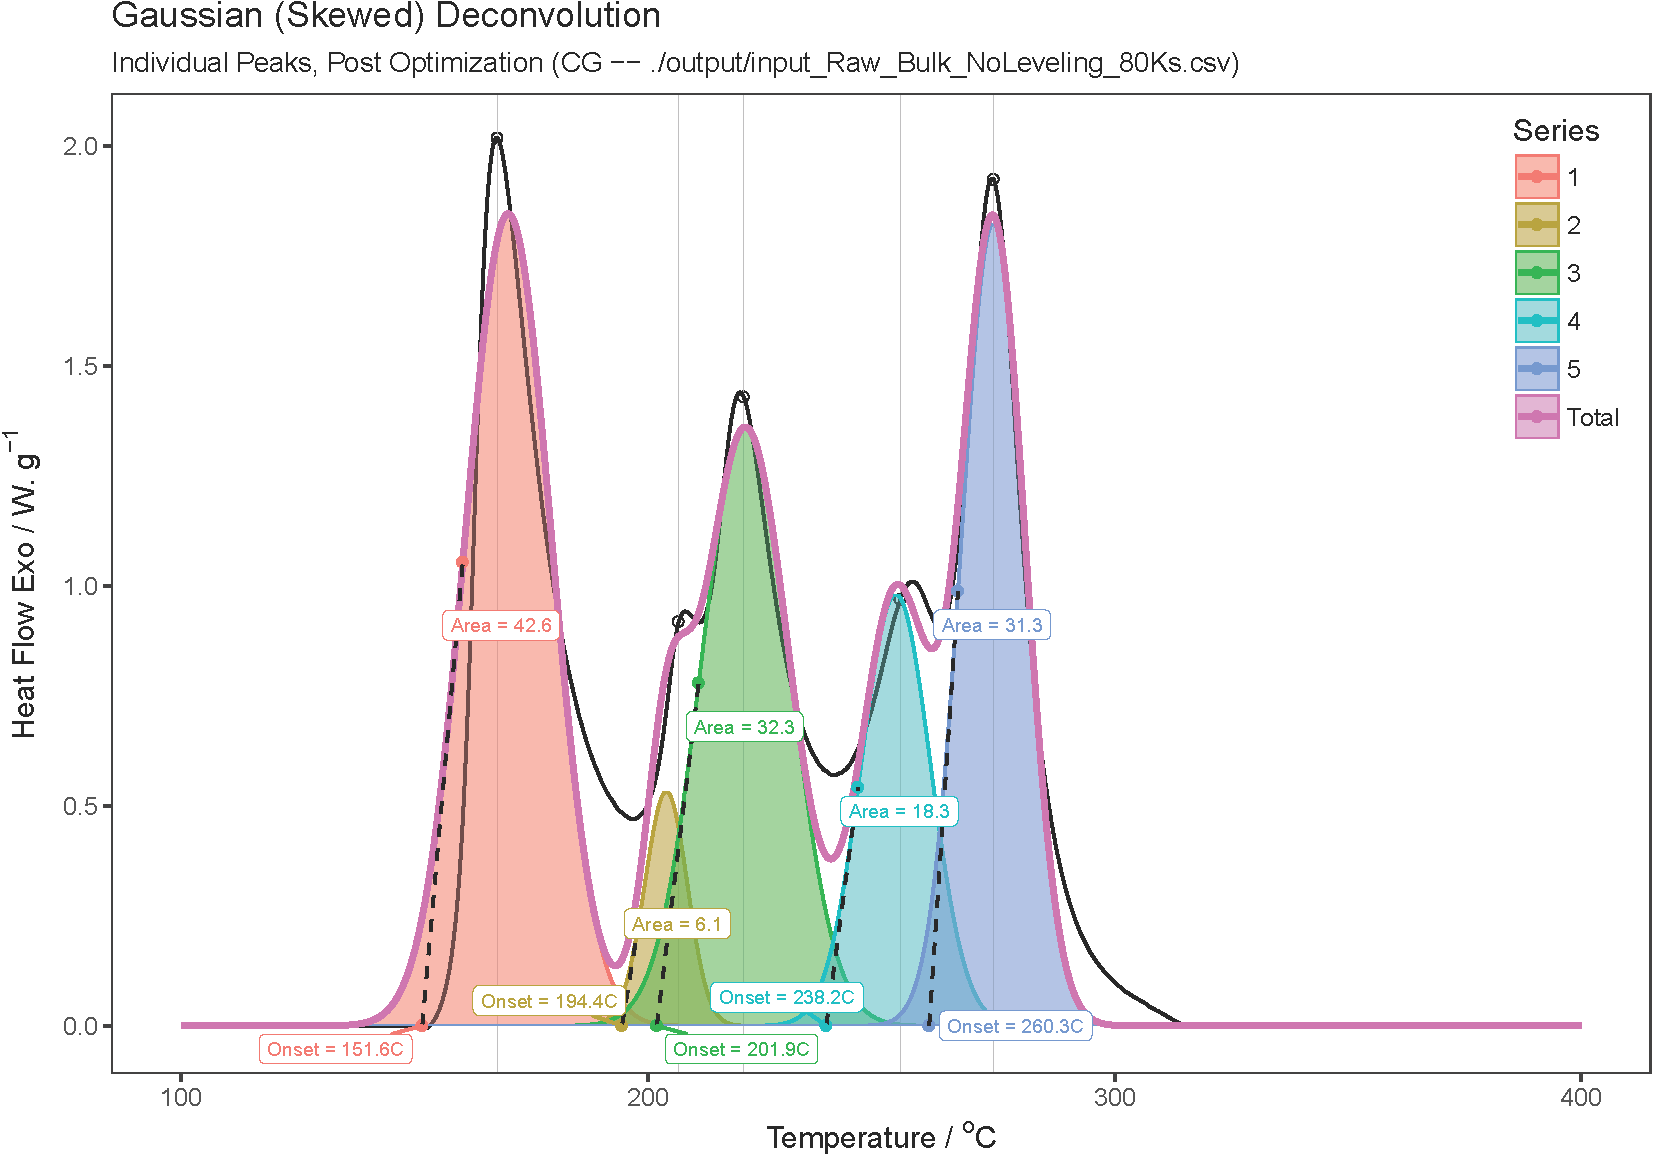
\includegraphics[width=.3\textwidth]{input_Raw_Bulk_NoLeveling_80Ks_result_A5lsc.png}\quad
	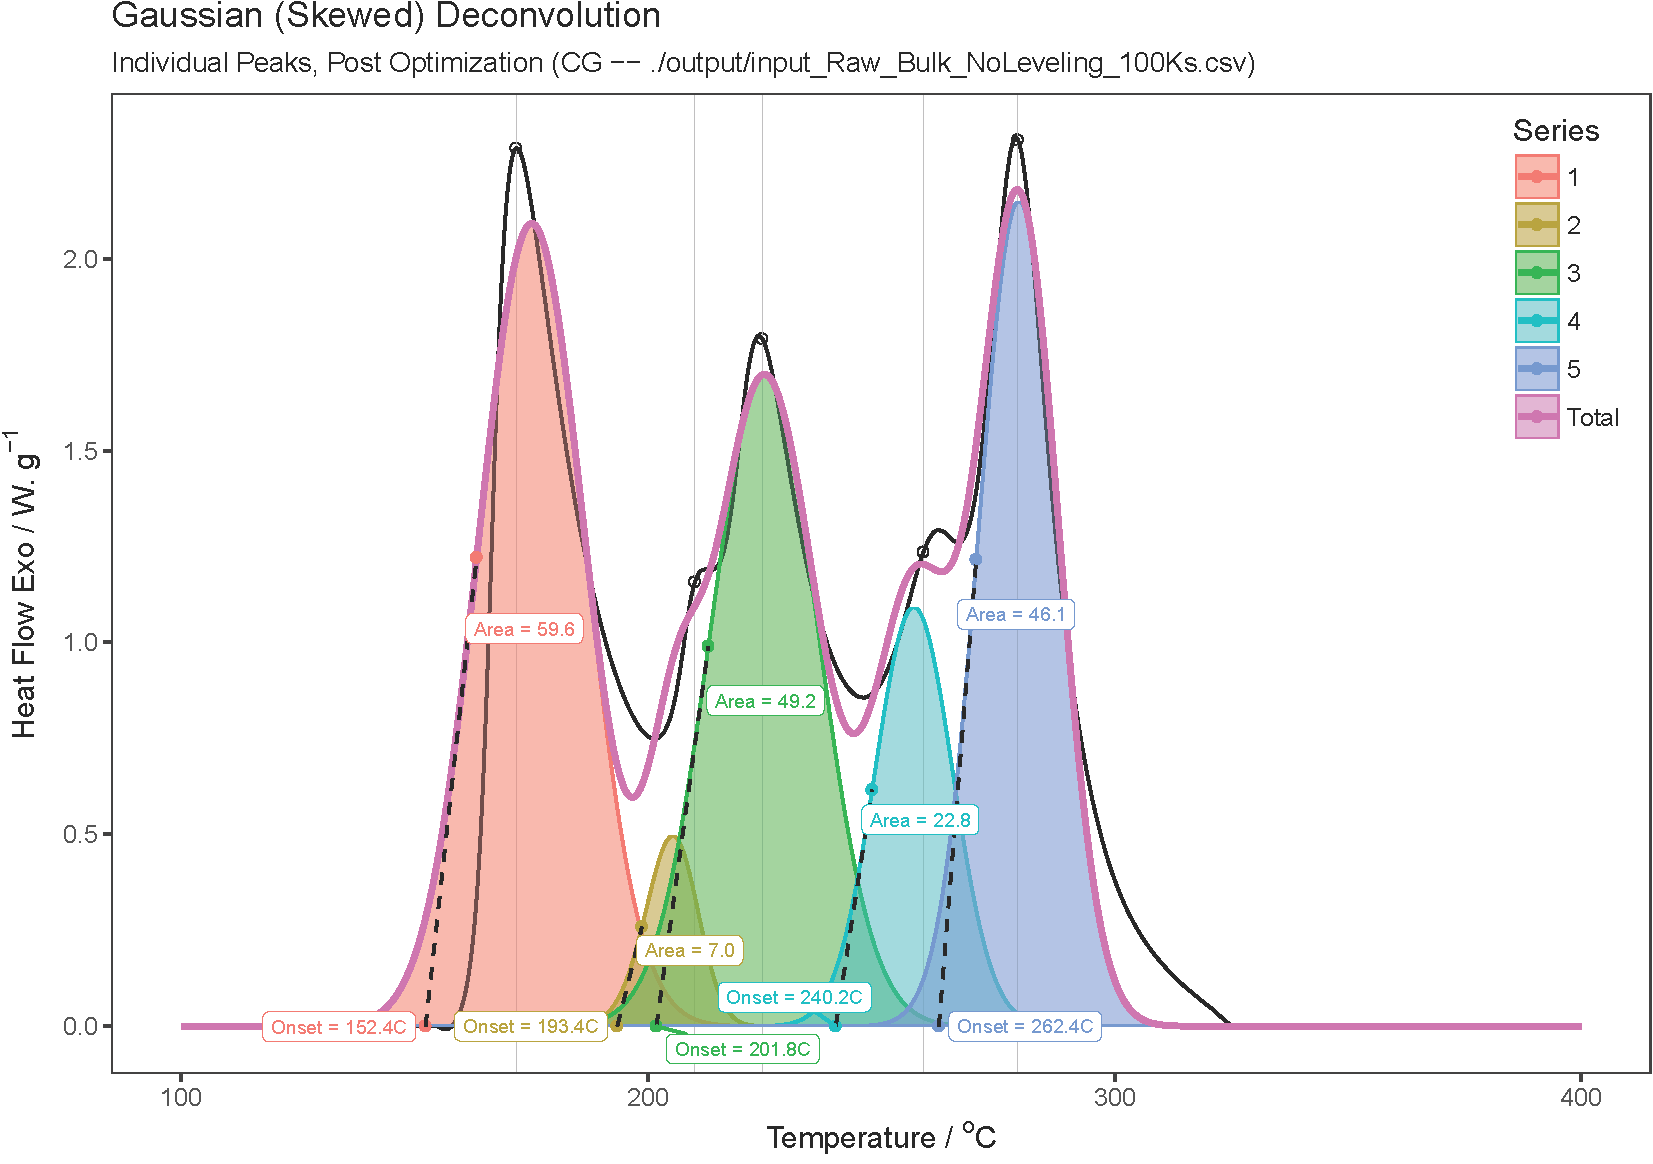
\includegraphics[width=.3\textwidth]{input_Raw_Bulk_NoLeveling_100Ks_result_A5lsc.png}
	\caption{\acrshort{dsc} deconvolution for the bulk at various \acrfullpl{ht}. From left to right, top to bottom, \gls{ht} = 5, 10, 15, 20, 30, 40, 60, 80, 100 $K/min$.}
	\label{fig:DSC_Bulk_Decon}
\end{figure}

%MultiFigure
\begin{figure}[b]
	\centering
	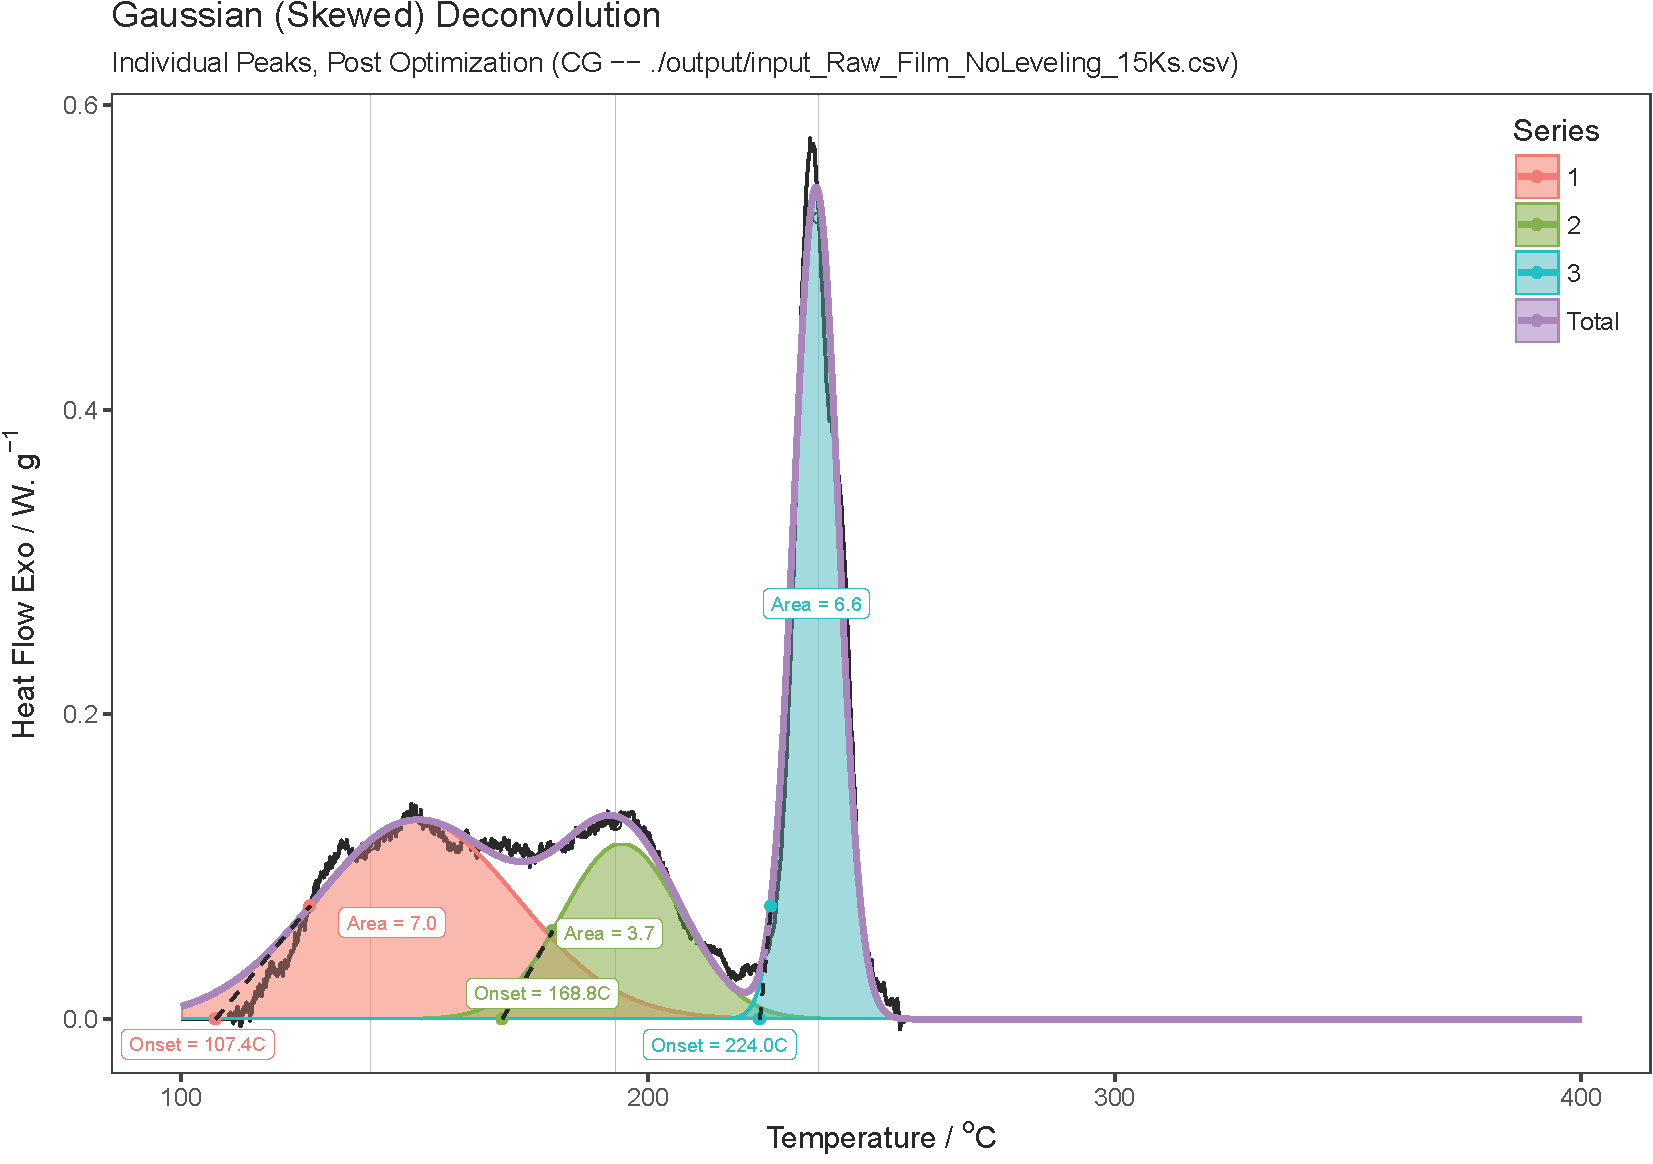
\includegraphics[width=.3\textwidth]{input_Raw_Film_NoLeveling_15Ks_result_A5lsc.png}\quad
	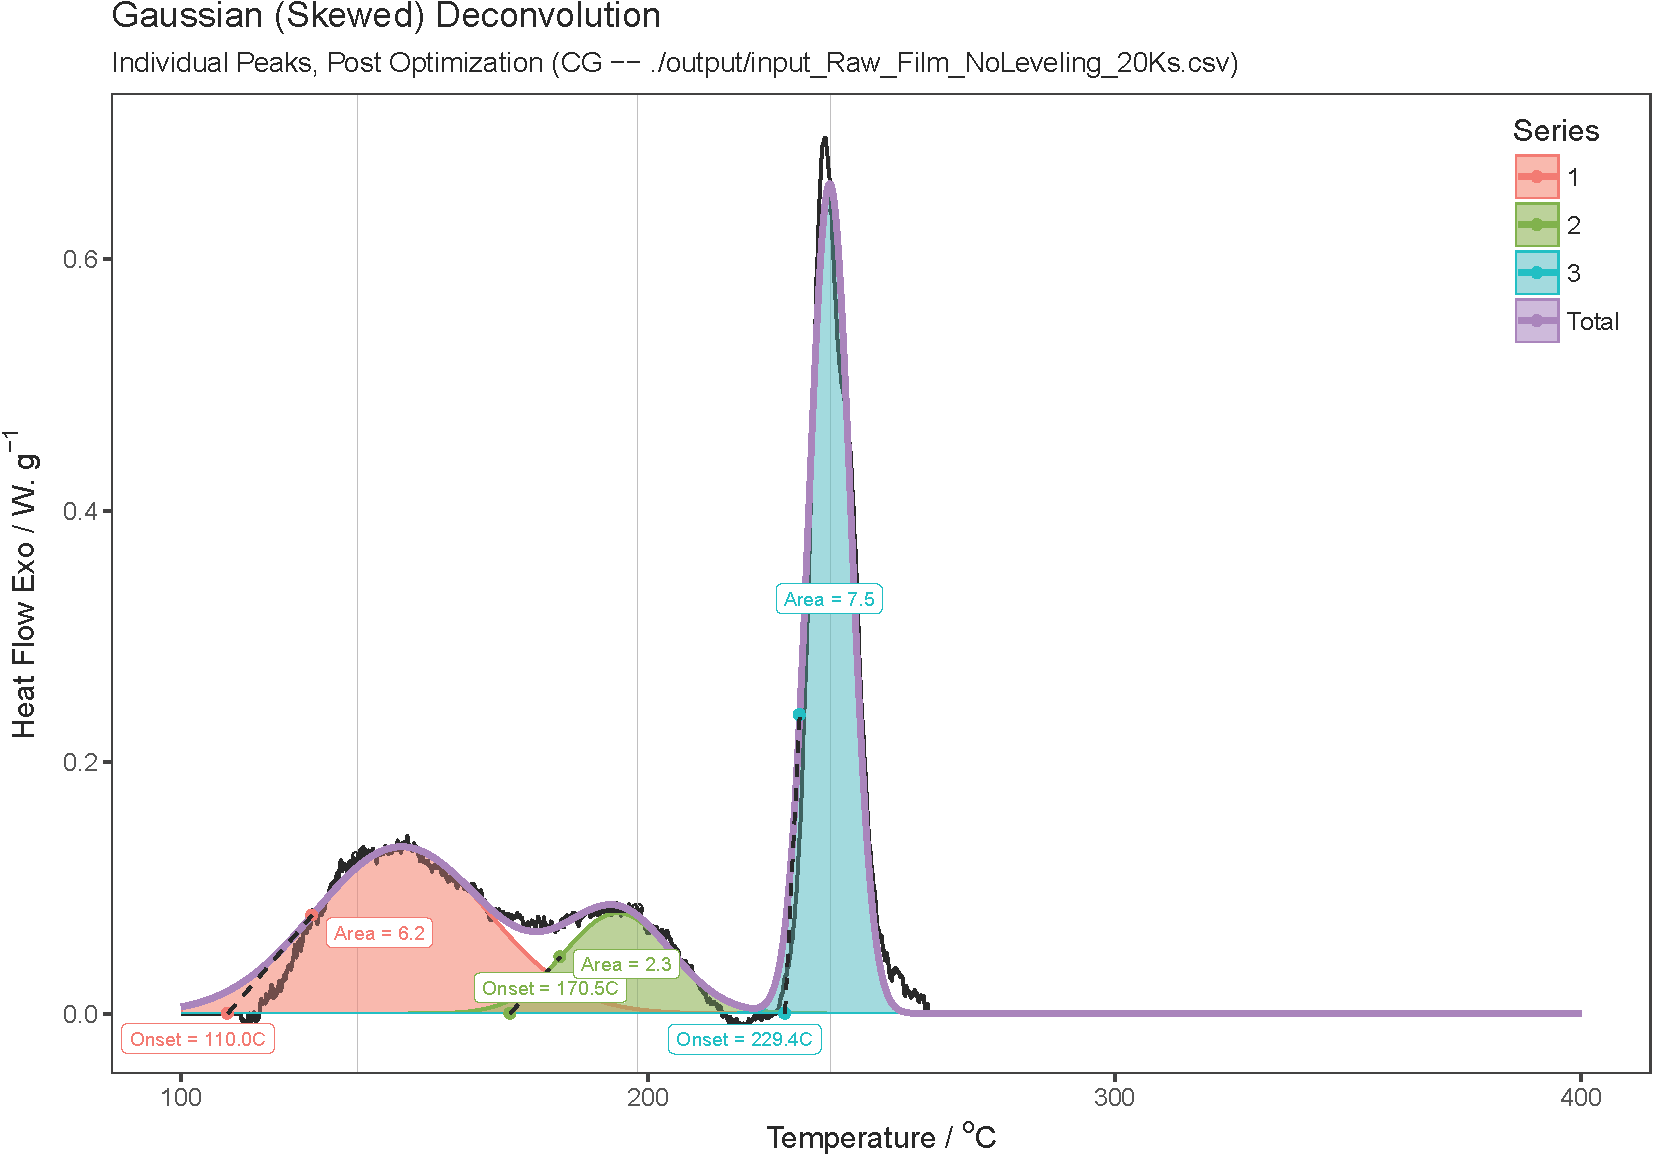
\includegraphics[width=.3\textwidth]{input_Raw_Film_NoLeveling_20Ks_result_A5lsc.png}\quad
	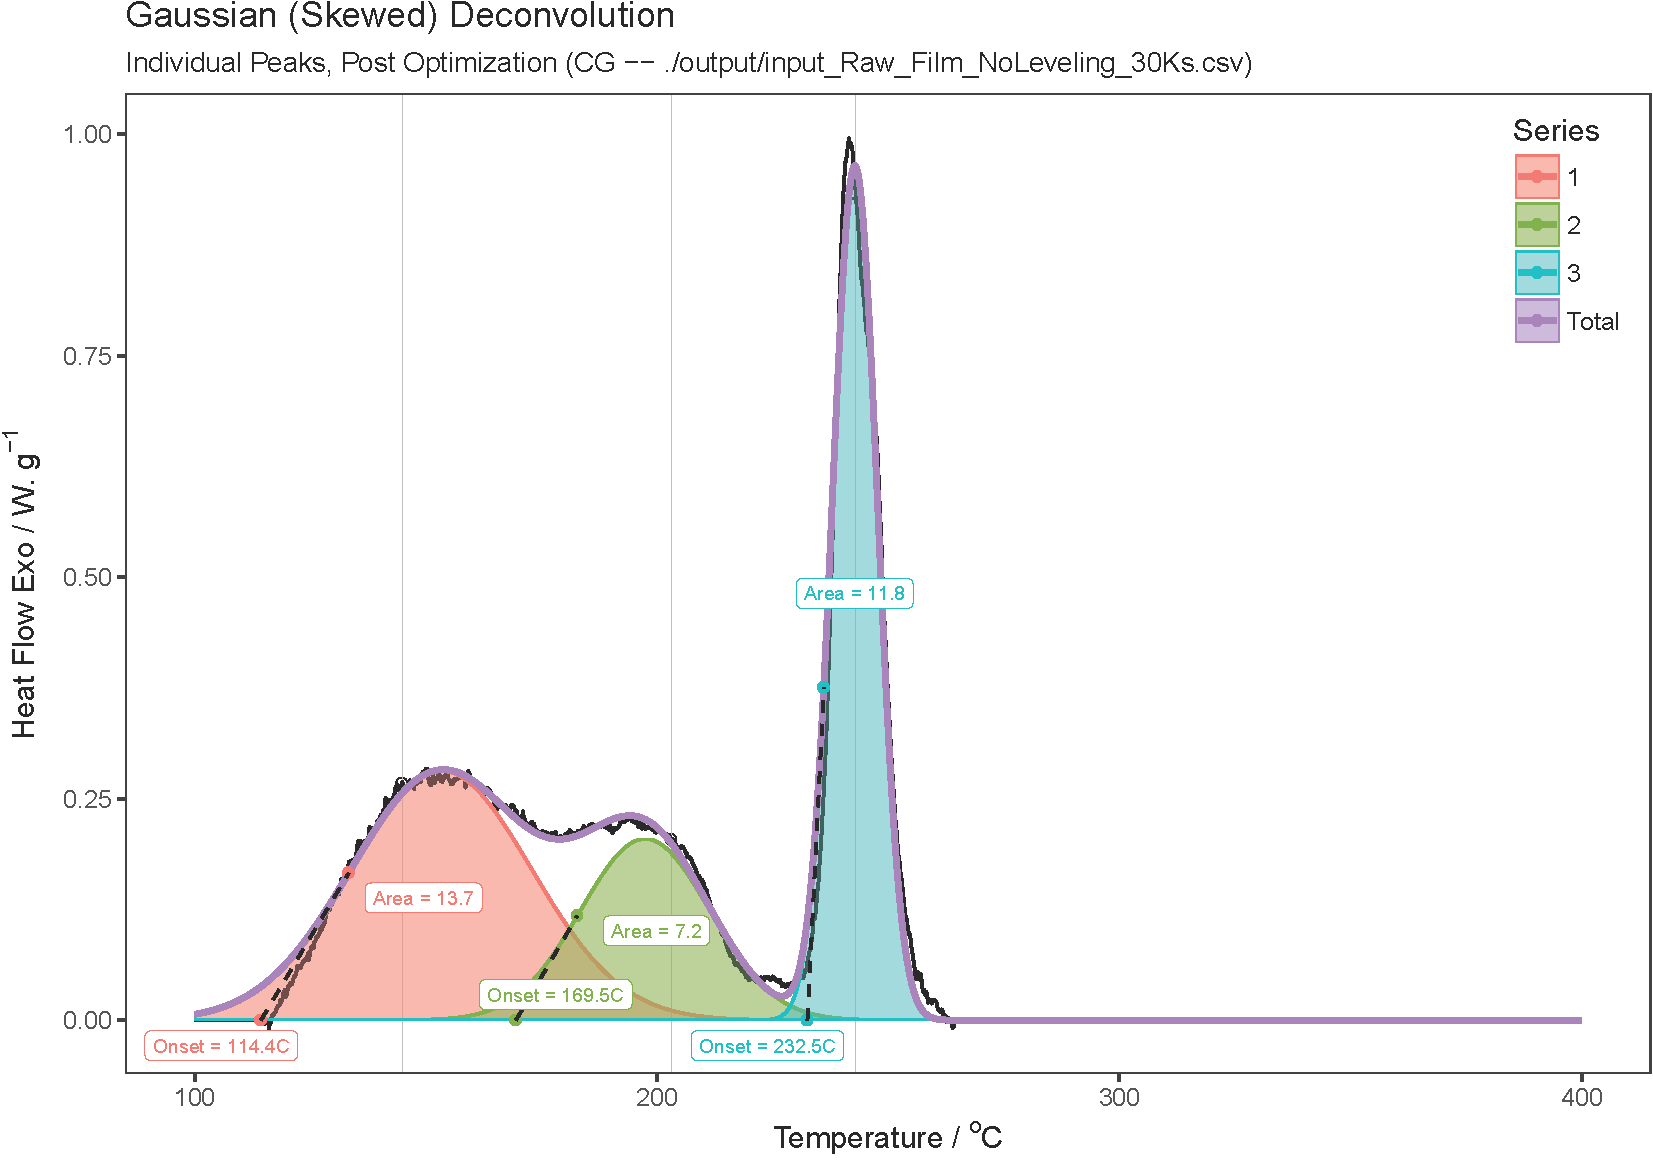
\includegraphics[width=.3\textwidth]{input_Raw_Film_NoLeveling_30Ks_result_A5lsc.png}
	\medskip
	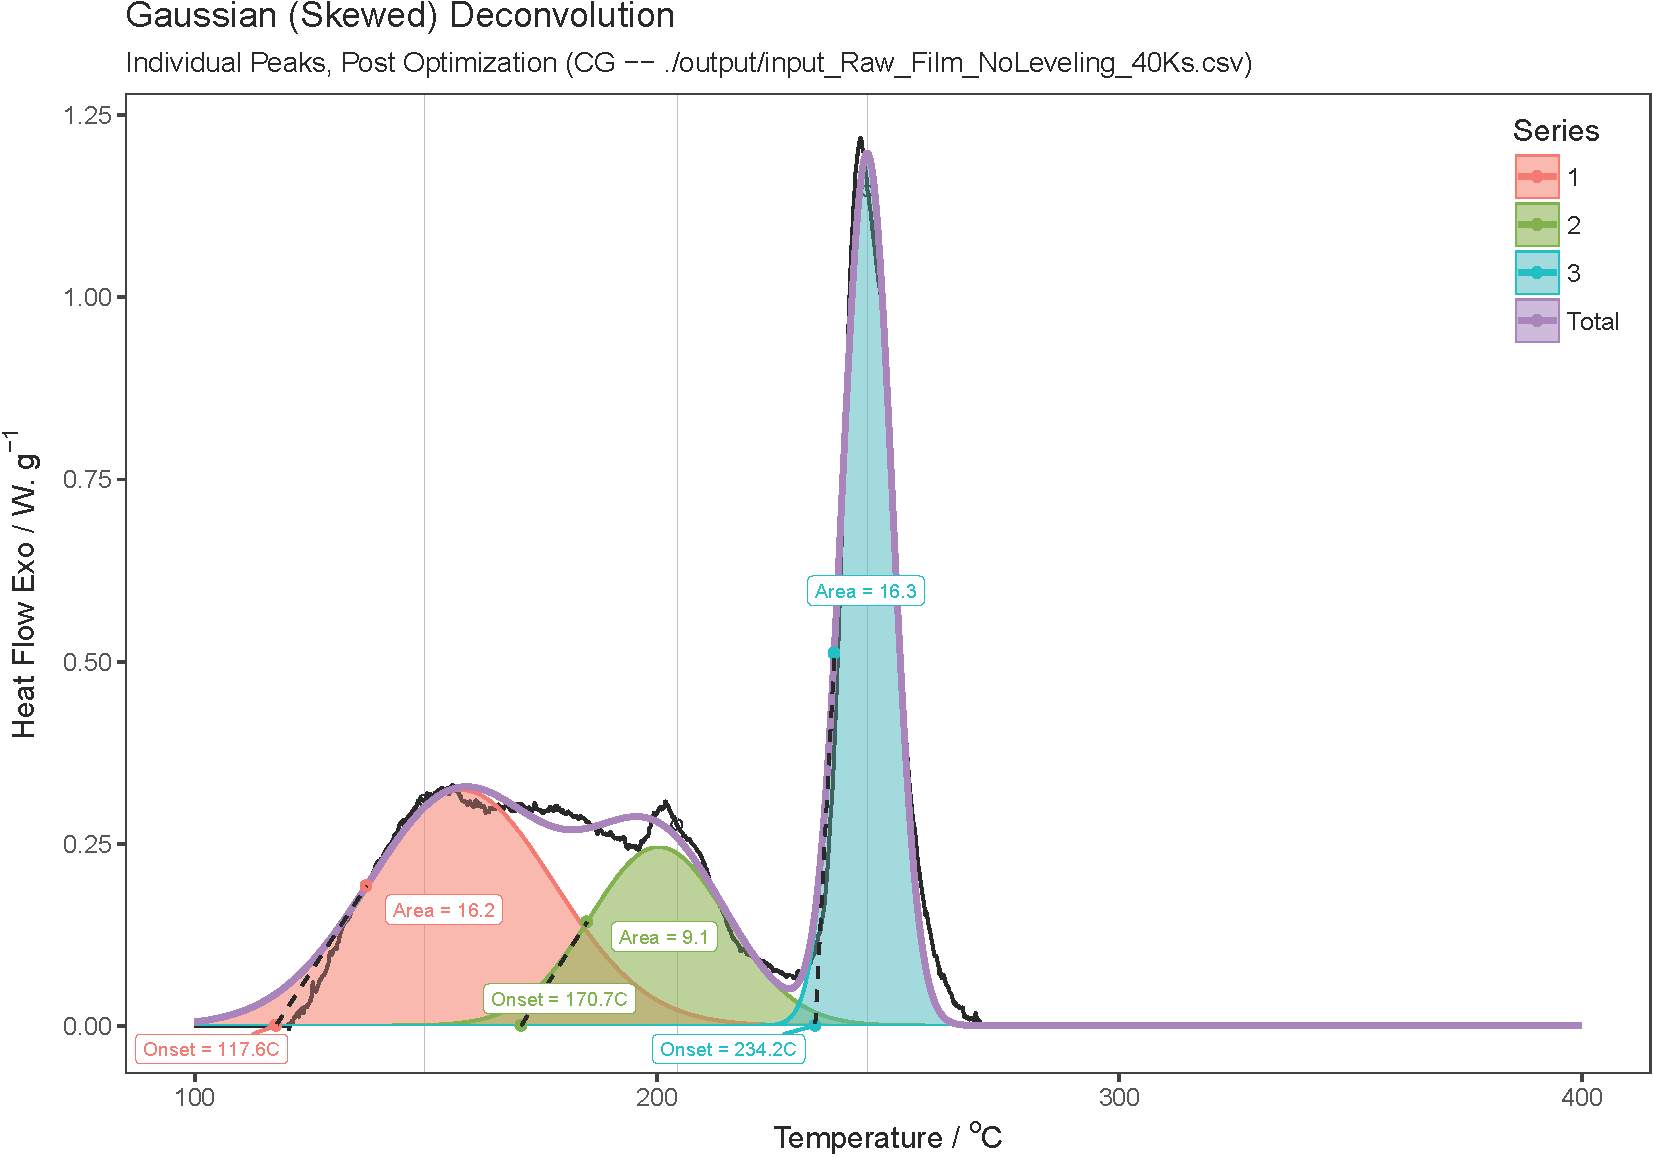
\includegraphics[width=.3\textwidth]{input_Raw_Film_NoLeveling_40Ks_result_A5lsc.png}\quad
	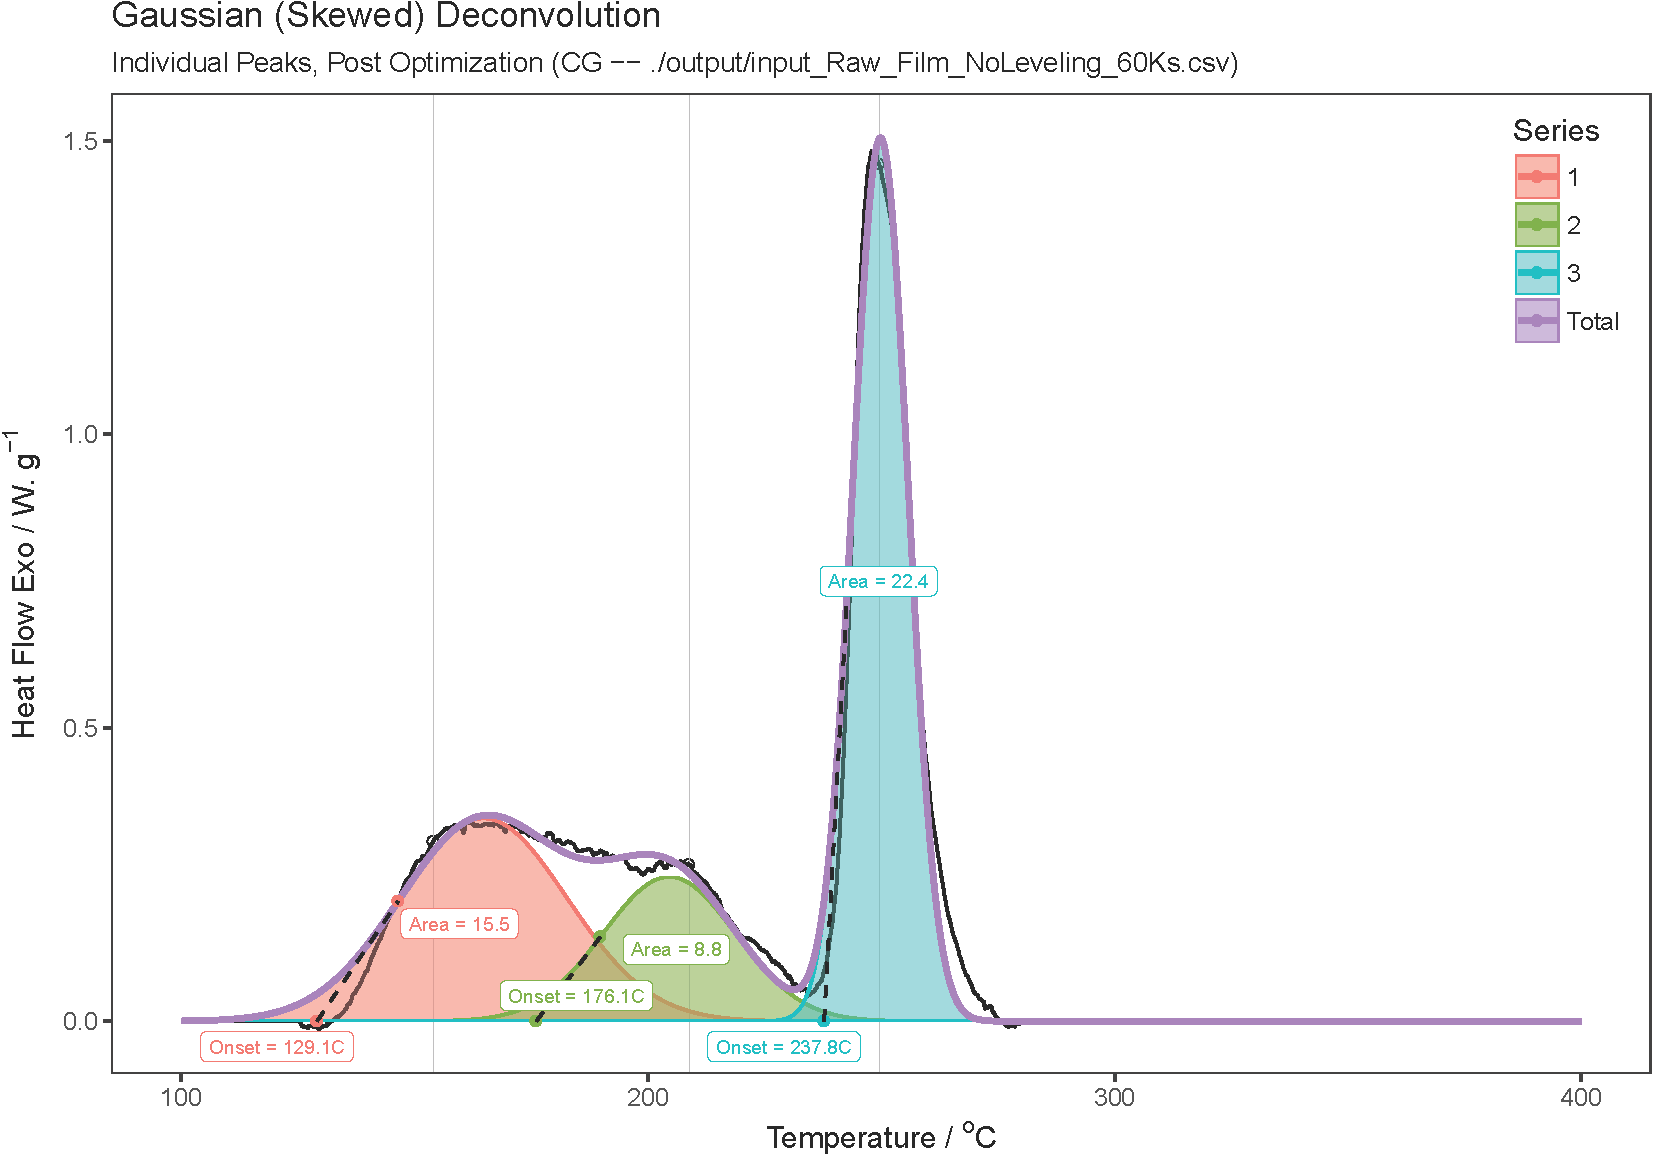
\includegraphics[width=.3\textwidth]{input_Raw_Film_NoLeveling_60Ks_result_A5lsc.png}\quad
	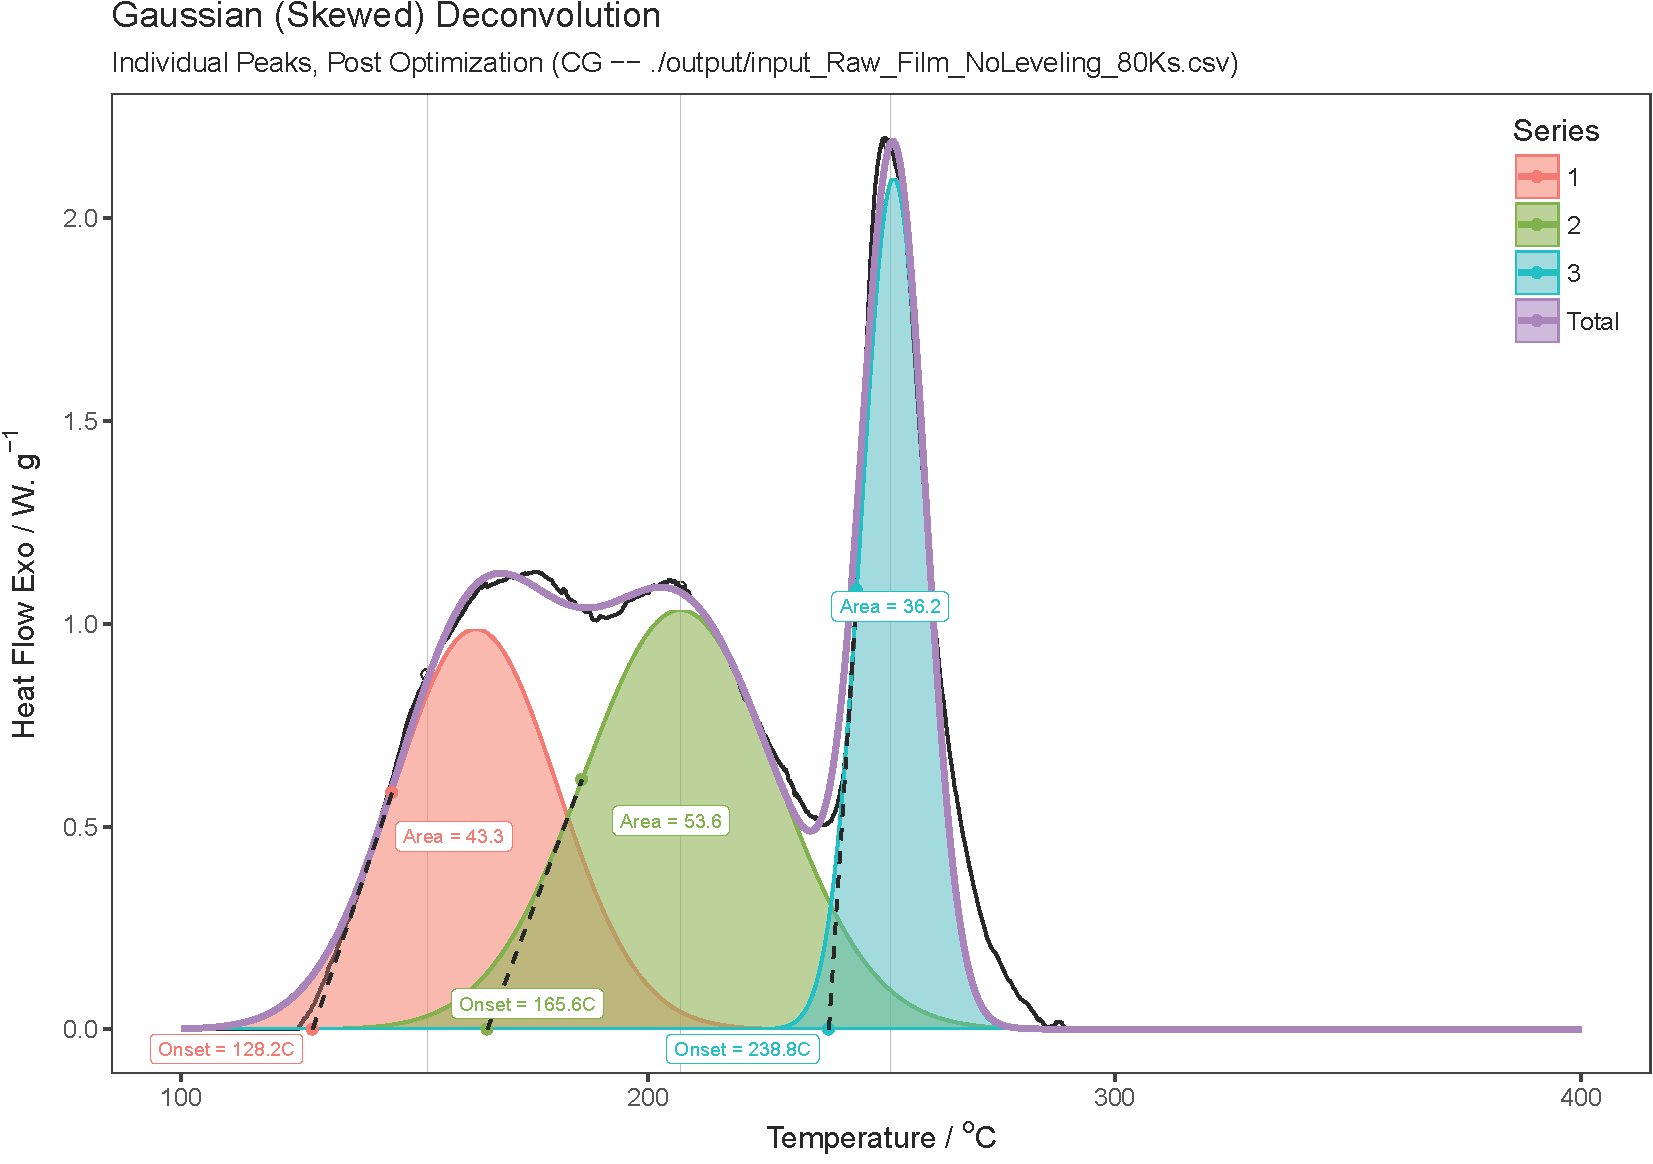
\includegraphics[width=.3\textwidth]{input_Raw_Film_NoLeveling_80Ks_result_A5lsc.png}
	\medskip
	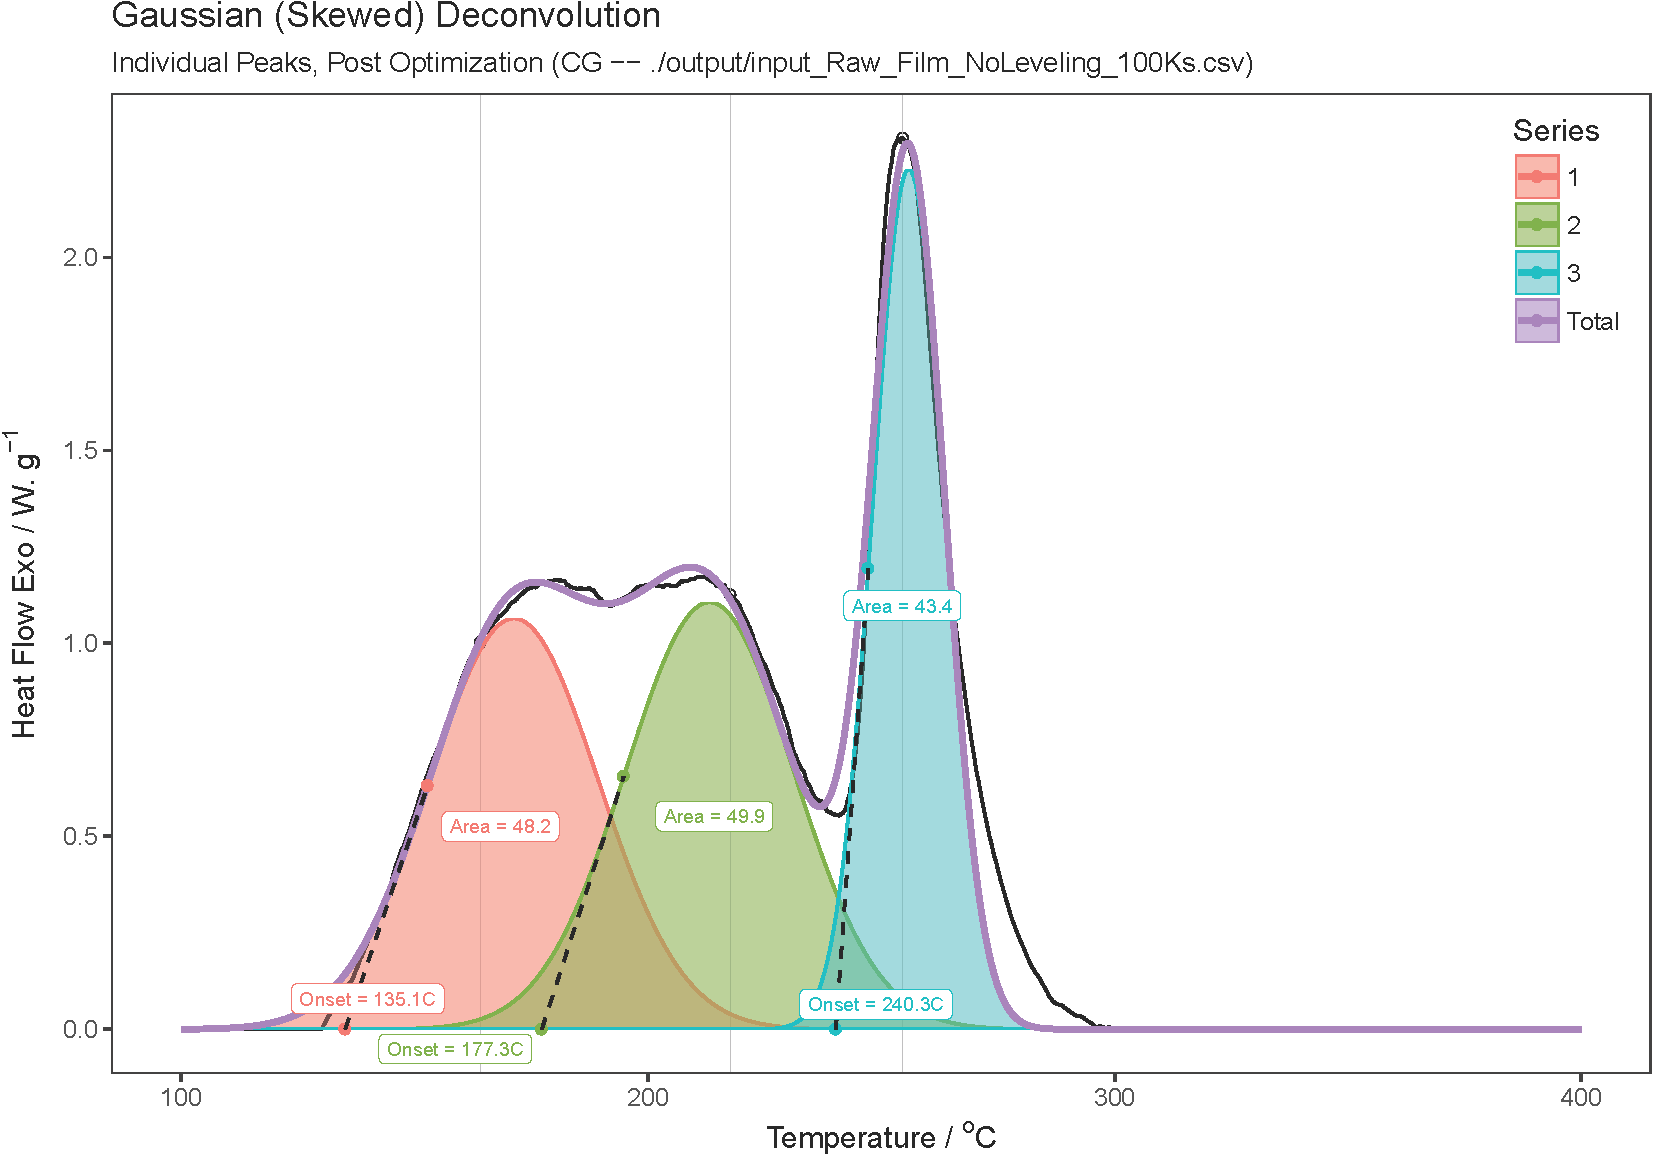
\includegraphics[width=.3\textwidth]{input_Raw_Film_NoLeveling_100Ks_result_A5lsc.png}
	\caption{\acrshort{dsc} deconvolution for the film at various \acrfullpl{ht}. From left to right, top to bottom, \gls{ht} = 15, 20, 30, 40, 60, 80, 100 $K/min$.}
	\label{fig:DSC_Film_Decon}
\end{figure}

\begin{table}[h]
	\centering
	\caption{Bulk \MgZnCa~ alloy onset temperatures for the various \acrshort{dsc} \acrfullpl{ht}. All temperatures are in \degree C.}
	\begin{tabular}{ c c c c c c c }
		\toprule
		Heating Rate \acrshort{ht} & \acrshort{Tg} & $T_{x1}$ & $T_{x2}$ & $T_{x3}$ & $T_{x4}$ & $T_{x5}$ \\ 
		$K/min$ & \degree C & \degree C & \degree C & \degree C & \degree C & \degree C \\
		\midrule
		100 & 136.1 & 164.8 & 193.4 & 201.8 & 240.2 & 262.4 \\
		80  & 132.0 & 160.0 & 194.4 & 201.9 & 238.2 & 260.3 \\
		60  & 129.6 & 157.7 & 190.0 & 197.8 & 232.9 & 259.0 \\
		40  & 126.6 & 155.2 & 189.0 & 200.0 & 226.4 & 254.7 \\
		30  & 126.2 & 151.5 & 187.0 & 198.4 & 221.0 & 251.1 \\
		20  & 125.1 & 149.8 & 188.4 & 197.0 & 216.0 & 246.8 \\
		15  & 123.8 & 148.3 & 186.2 & 195.6 & 212.2 & 243.9 \\
		10  & 123.5 & 144.5 & 183.4 & 192.9 & 207.4 & 239.8 \\
		5   & 120.5 & 141.1 & 179.7 & 187.5 & 199.8 & 232.7 \\ 
		\bottomrule
	\end{tabular}
	\label{tab:BulkOnsets}
\end{table}

\begin{table}[h]
	\centering
	\caption{Film \MgZnCa~ alloy onset temperatures for the various \acrshort{dsc} \acrfullpl{ht}. All temperatures are in \degree C.}
	\begin{tabular}{ c c c c c c c }
		\toprule
		Heating Rate \acrshort{ht} & \acrshort{Tg} & $T_{x1}$ & $T_{x2}$ & $T_{x3}$ & $T_{x4}$ & $T_{x5}$ \\ 
		$K/min$  & \degree C & \degree C & \degree C & \degree C & \degree C & \degree C \\
		\midrule
		100 & 108.5 & 128.6 &  & 177.3 &  & 240.3 \\
		80  & 106.0 & 121.2 &  & 165.6 &  & 238.8 \\
		60  & 107.3 & 134.0 &  & 176.1 &  & 237.8 \\
		40  & 100.2 & 119.8 &  & 170.7 &  & 234.2 \\
		30  & 95.3  & 110.4 &  & 169.5 &  & 232.5 \\
		20  & 95.5  & 115.2 &  & 170.5 &  & 229.4 \\
		15  & 92.5  & 113.5 &  & 168.8 &  & 224.0 \\
		\bottomrule
	\end{tabular}
	\label{tab:FilmOnsets}
\end{table}

%single image
\begin{figure}[b]
	\centering
	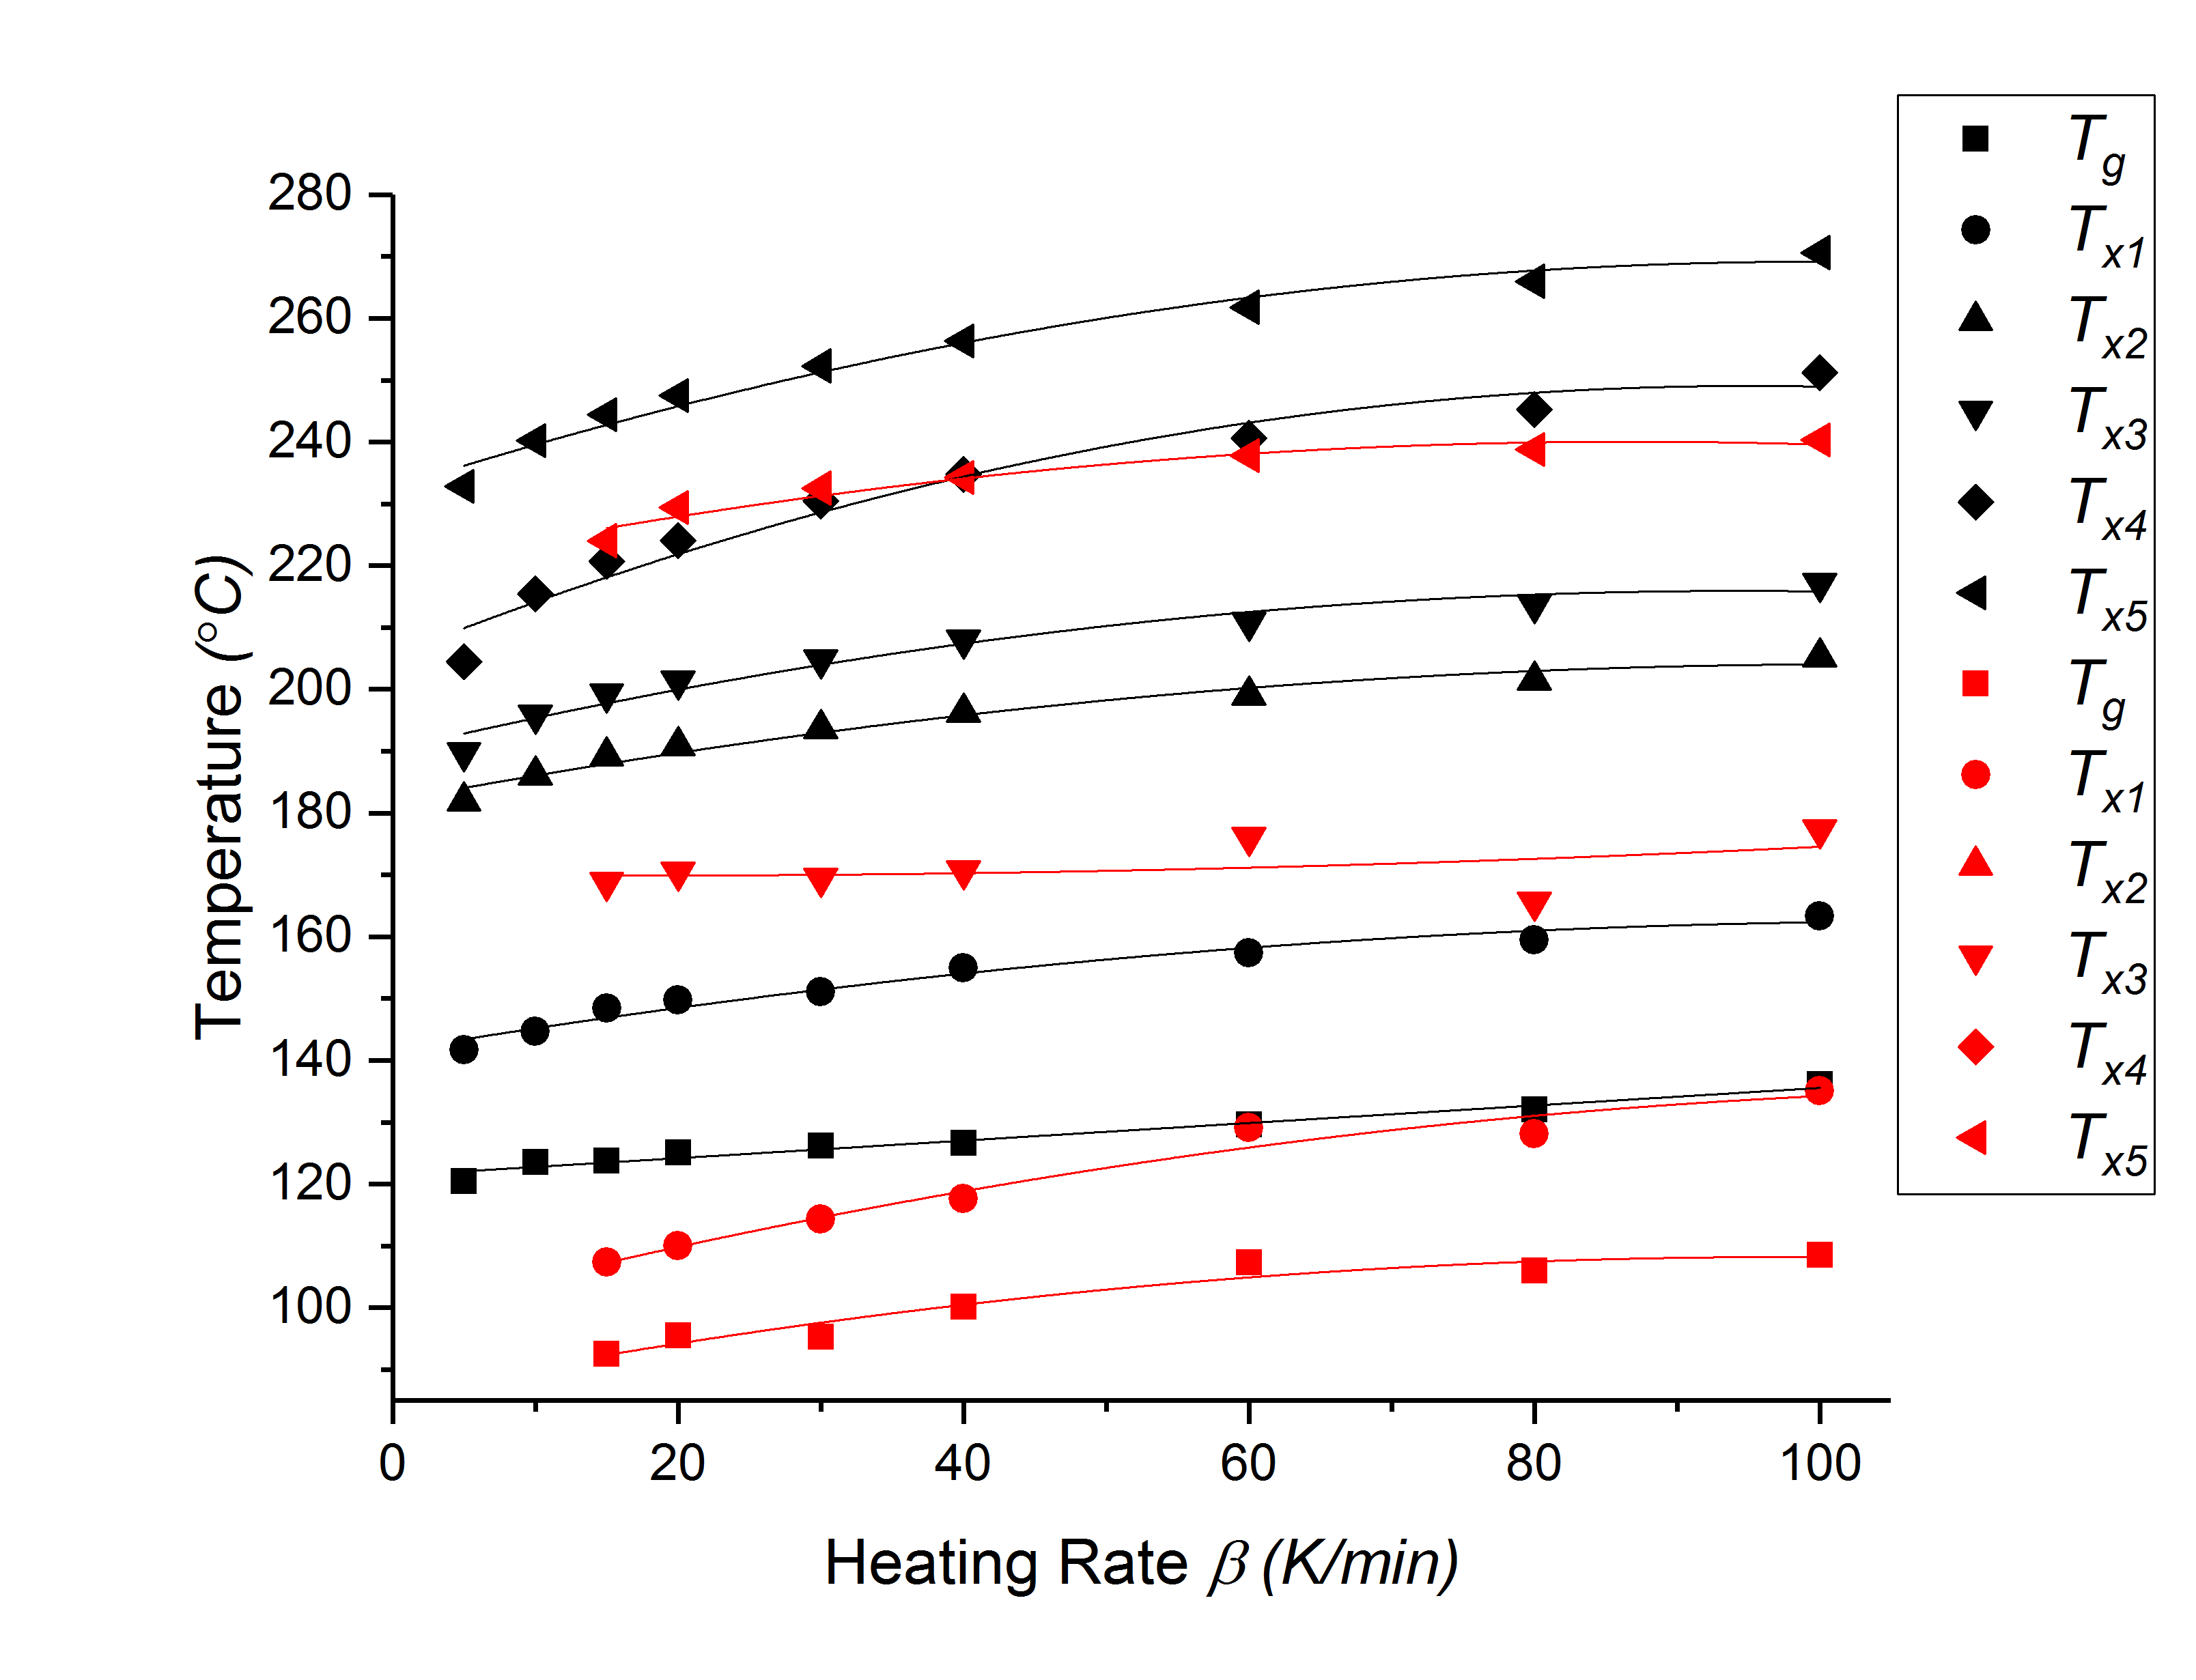
\includegraphics[width=0.55\textwidth]{Onsets_BulkandFilm.png}
	\caption[Table of contents Capition]{The \Tg s and \Tx s plotted at each \acrshort{dsc} \acrfull{ht} for both the bulk and film \MgZnCa. Bulk is shown in black, and film in red.}%global caption
	\label{fig:DSC_Onsets_BulkFilm}
\end{figure}

\subsubsection{Reaction enthalpy}

The deconvolution fits were integrated to find the area under each curve. This information provides the \gls{h} of the crystallisation formation of each phase. These energies are presented in Tables \ref{tab:Bulk_Enthalpy} and \ref{tab:Film_Enthalpy} for the bulk and film respectively. Figure \ref{fig:DSC_Decon} shows the \Tx~ onsets and \acrfull{h} for both the bulk and film plotted together.

From Tables \ref{tab:Bulk_Enthalpy} and \ref{tab:Film_Enthalpy}, and Figure \ref{fig:DSC_Decon} it can be seen most of the crystallisation formation energy is needed to form the $1^{st}$, $3^{rd}$, and $5^{th}$ phases (i.e. \Tx $_{1, 3, 5}$). With these three phases accounting for approximately $73 \pm 7\%$ of the bulk crystallisation energy. The total crystallisation energy of these three bulk phases is also similar to the total energy for the films. Demonstrating that the bulk requires more energy to crystallize than the films. 
\todo{This is what ISMANAM scientist said would be expected from a not USG glass. i.e. this is the typical expectation [sources needs].} 

\begin{table}[h]
	\centering
	\caption{Bulk \MgZnCa~ alloy \acrfull{h} of crystallisation formation for $Tx_{1-5}$ for the various \acrshort{dsc} \acrfullpl{ht}; \gls{h} is in $J/g$.}
	\begin{tabular}{ c c c c c c c }
		\toprule
		Heating Rate \acrshort{ht} & $h_{T_{x1}}$ & $h_{T_{x2}}$ & $h_{T_{x3}}$ & $h_{T_{x4}}$ & $h_{T_{x5}}$ & $h_{Total}$ \\ 
		$K/min$ & $J/g$ & $J/g$ & $J/g$ & $J/g$ & $J/g$ & $J/g$ \\
		\midrule
		100 & 59.59 & 6.97 & 49.16 & 22.84 & 46.08 & 184.64 \\
		80  & 42.61 & 6.08 & 32.33 & 18.27 & 31.25 & 130.54 \\
		60  & 30.02 & 4.05 & 25.41 & 16.76 & 19.81 & 96.05  \\
		40  & 16.93 & 4.36 & 12.44 & 11.13 & 11.68 & 56.54  \\
		30  & 12.03 & 3.68 & 9.32  & 9.18  & 9.02  & 43.23  \\
		20  & 7.18  & 2.21 & 4.99  & 5.67  & 5.78  & 25.83  \\
		15  & 5.48  & 2.01 & 3.65  & 4.69  & 4.43  & 20.26  \\
		10  & 3.45  & 1.43 & 2.28  & 3.14  & 2.92  & 13.22  \\
		5   & 1.65  & 0.69 & 1.09  & 1.47  & 1.42  & 6.32   \\
		\bottomrule
	\end{tabular}
	\label{tab:Bulk_Enthalpy}
\end{table}

\begin{table}[h]
	\centering
	\caption{Film \MgZnCa~ alloy \acrfull{h} of crystallisation formation for $Tx_{1-5}$ for the various \acrshort{dsc} \acrfullpl{ht}; \gls{h} is in $J/g$.}
	\begin{tabular}{ c c c c c c c }
		\toprule
		Heating Rate \acrshort{ht} & $h_{T_{x1}}$ & $h_{T_{x2}}$ & $h_{T_{x3}}$ & $h_{T_{x4}}$ & $h_{T_{x5}}$ & $h_{Total}$ \\ 
		$K/min$ & $J/g$ & $J/g$ & $J/g$ & $J/g$ & $J/g$ & $J/g$ \\
		\midrule
		100 & 48.24 &  & 49.85 &  & 43.38 & 141.47 \\
		80  & 43.27 &  & 53.56 &  & 36.18 & 133.01 \\
		60  & 15.5  &  & 8.78  &  & 22.4  & 46.68  \\
		40  & 16.22 &  & 9.13  &  & 16.27 & 41.62  \\
		30  & 13.72 &  & 7.16  &  & 11.81 & 32.69  \\
		20  & 6.16  &  & 2.3   &  & 7.45  & 15.91  \\
		15  & 6.99  &  & 3.66  &  & 6.57  & 17.22  \\
		\bottomrule
	\end{tabular}
	\label{tab:Film_Enthalpy}
\end{table}

%MultiFigure
\begin{figure}[b]
	\centering
	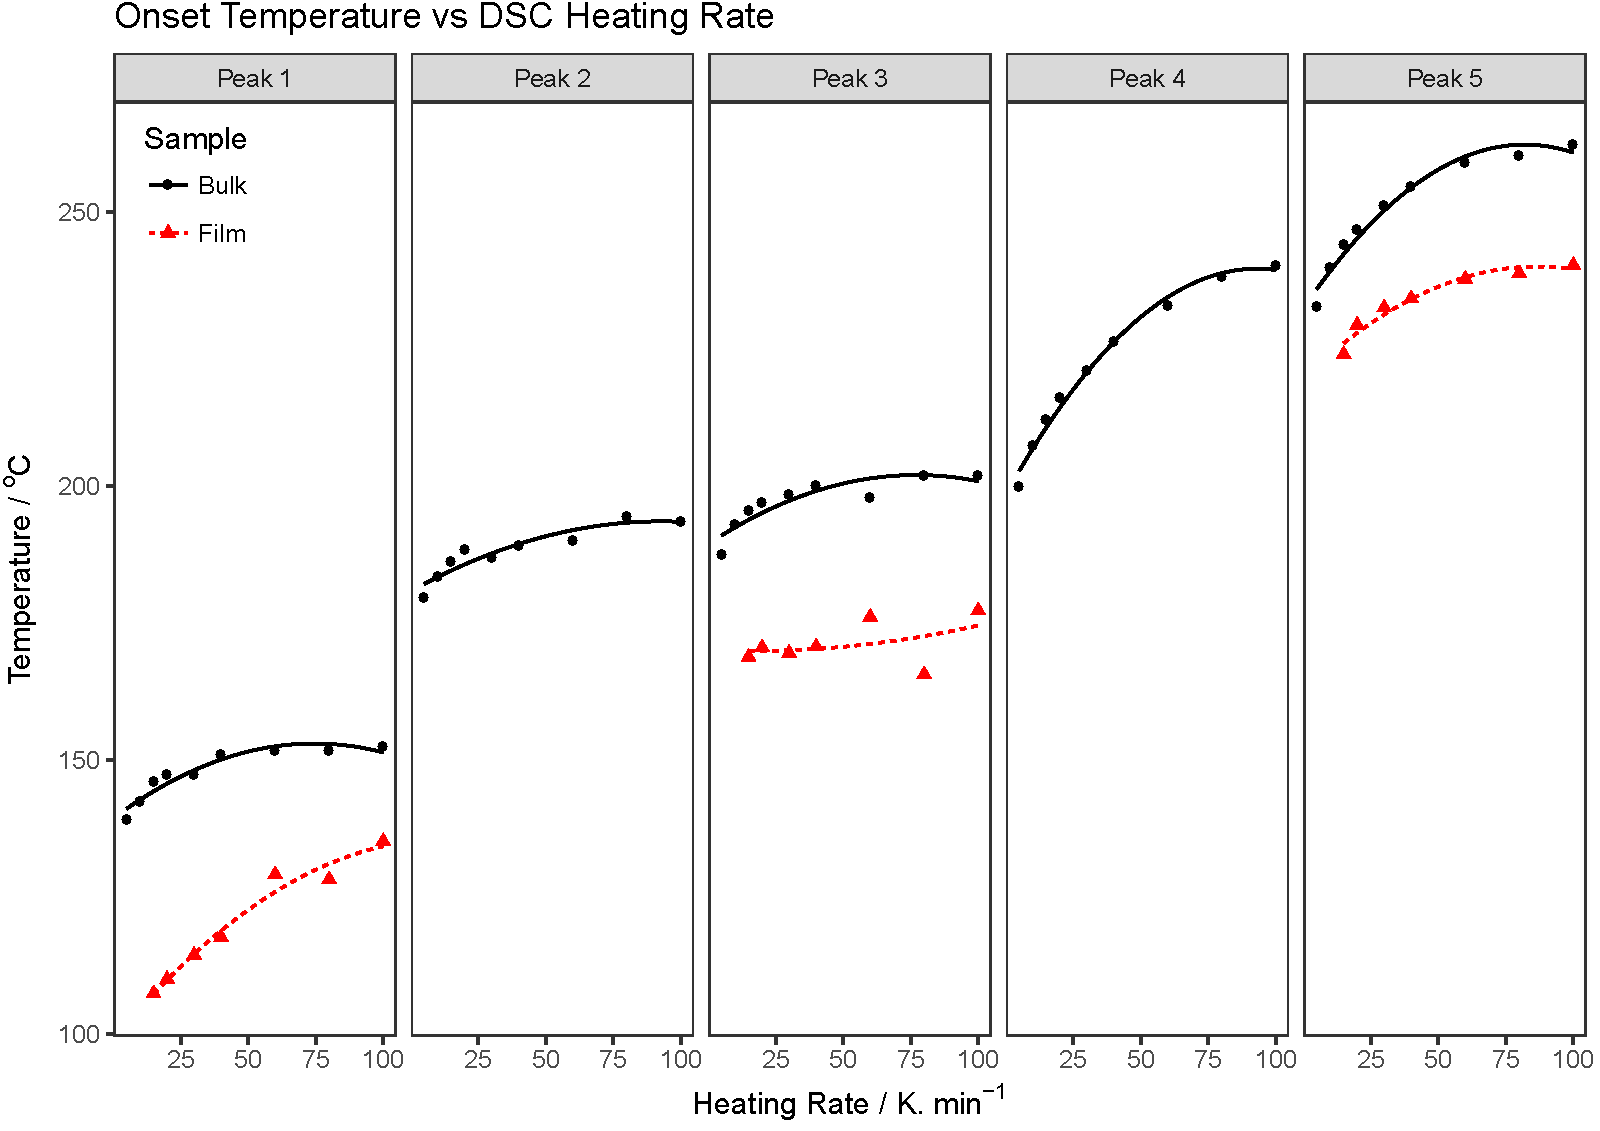
\includegraphics[width=.6\textwidth]{Decon_Onsets_BR.png}
	\medskip
	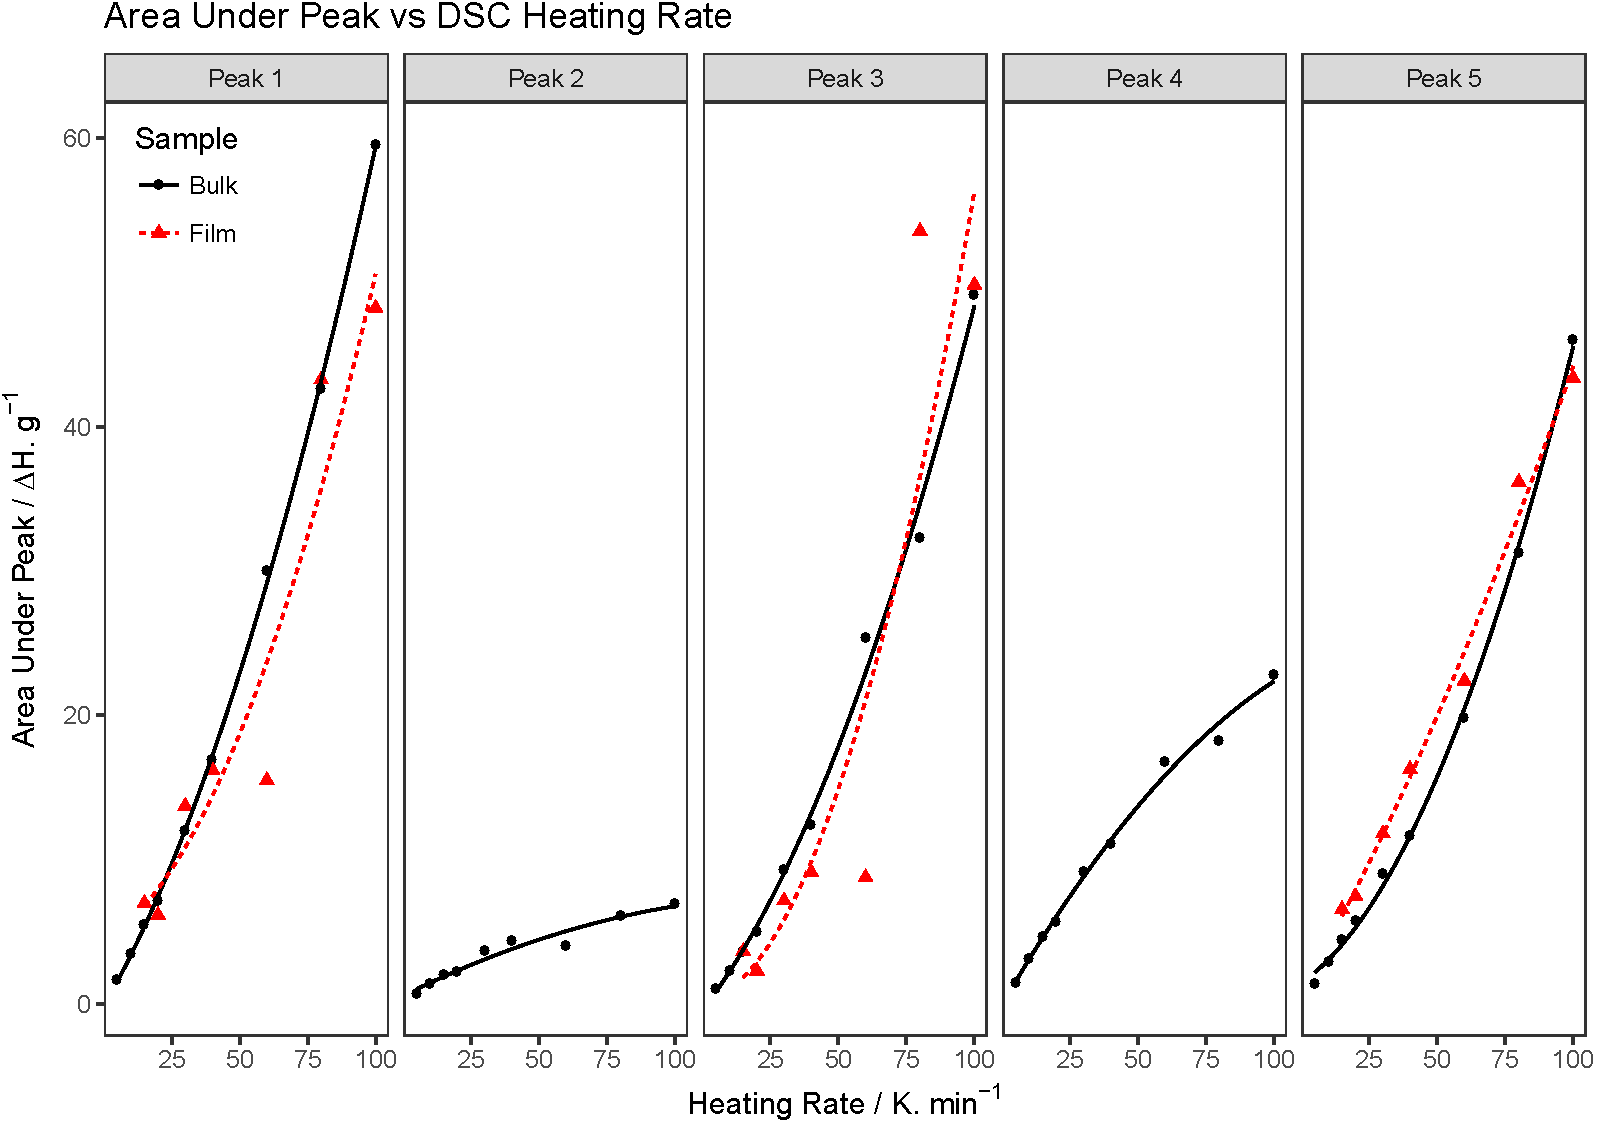
\includegraphics[width=.6\textwidth]{Decon_peak_area_BR.png}
	\caption{\acrshort{dsc} \Tx~ onset temperatures and \acrfull{h} of crystallisation formation for the bulk and film at each \acrfull{ht}. Bulk is shown in black, and film in red.}
	\label{fig:DSC_Decon}
\end{figure}

\subsubsection{Relaxation enthalpy}

For next paper on relaxation / rejuvenation.

\subsection{\acrshort{xrd}}
\subsubsection{Annealing \acrshort{xrd}}

The crystallisation events observed and deconvoluted from the \acrshort{dsc} were further examined with annealing \acrshort{xrd}. Both the bulk and film were heat treated by annealing to 120, 140, 145, 170, 200, 250, 290, and 320\degree C before \acrshort{xrd}. This allowed for the location of the \Tg~ and \Tx s to be confirmed as well as for the crystallisation phases to be identify.

From these experiments 5 previously observed crystallisation phases of the MgZnCa system \cite{Zhang2013, Zhang2012, Zhang2011, Khan1989, Cao2016} were characterised in the bulk and film \MgZnCa. This allowed the crystallisation process of \MgZnCa~ from the fully amorphous glass to fully crystalline metal to be identified as;

\centerline{Glass $\rightarrow$ Mg$_{51}$Zn$_{20}$ $\rightarrow$ Mg $\rightarrow$ Ca$_{2}$Mg$_{5}$Zn$_{5}$ $\rightarrow$ MgZn $\rightarrow$ Ca$_{2}$Mg$_{5}$Zn$_{13}$}

The annealing \acrshort{xrd} results are shown in Figures \ref{fig:XRD_Annealing_Bulk} and \ref{fig:XRD_Annealing_Film} for the bulk and film respectively. In these figures each phase is identified with a tracer at the temperature it was most strongly observed. Note the Al substrates peaks have been faceted in Figure \ref{fig:XRD_Annealing_Film} as to not dwarf the other peaks. 

In Figures \ref{fig:XRD_Annealing_Bulk} and \ref{fig:XRD_Annealing_Film} it can be observed that Mg$_{51}$Zn$_{20}$ comes out at lower temperature in the film compared to the bulk, while the other phases nucleate and grow at similar rates for both the bulk and film. The temperature each phase is first and last observed are tabulated in Table \ref{tab:Crystal_Sequence}. 

\begin{table}[h]
	\centering
	\caption{Temperatures at which each crystallisation phase is first observed and last observed in the annealing \acrshort{xrd} for both the bulk and film. All temperatures are in \degree C.}
	\begin{tabular}{ c c c c c }
		\toprule
		Phase & \multicolumn{2}{c}{Bulk} & \multicolumn{2}{c}{Film}                 \\
		& First Temp & Last Temp & First Temp & Last Temp \\
		\midrule
		Glass 						& 35 & 200 & 35 & 200 \\
		Mg$_{51}$Zn$_{20}$ \cite{Zhang2013, Khan1989} & 170 & 200 & 140 & 200 \\
		Mg 							& 170 & 320 & 140 & 320 \\
		Ca$_{2}$Mg$_{5}$Zn$_{5}$ \cite{Zhang2013, Cao2016} & 200 & 250 & 200 & 250 \\
		MgZn \cite{Khan1989} & 250 & 250 & 250 & 250 \\
		Ca$_{2}$Mg$_{5}$Zn$_{13}$ \cite{Zhang2013, Zhang2012, Zhang2011} & 290 & 320 & 290 & 320 \\
		\bottomrule
	\end{tabular}
	\label{tab:Crystal_Sequence}
\end{table}

%single image
\begin{figure}[b]
	\centering
	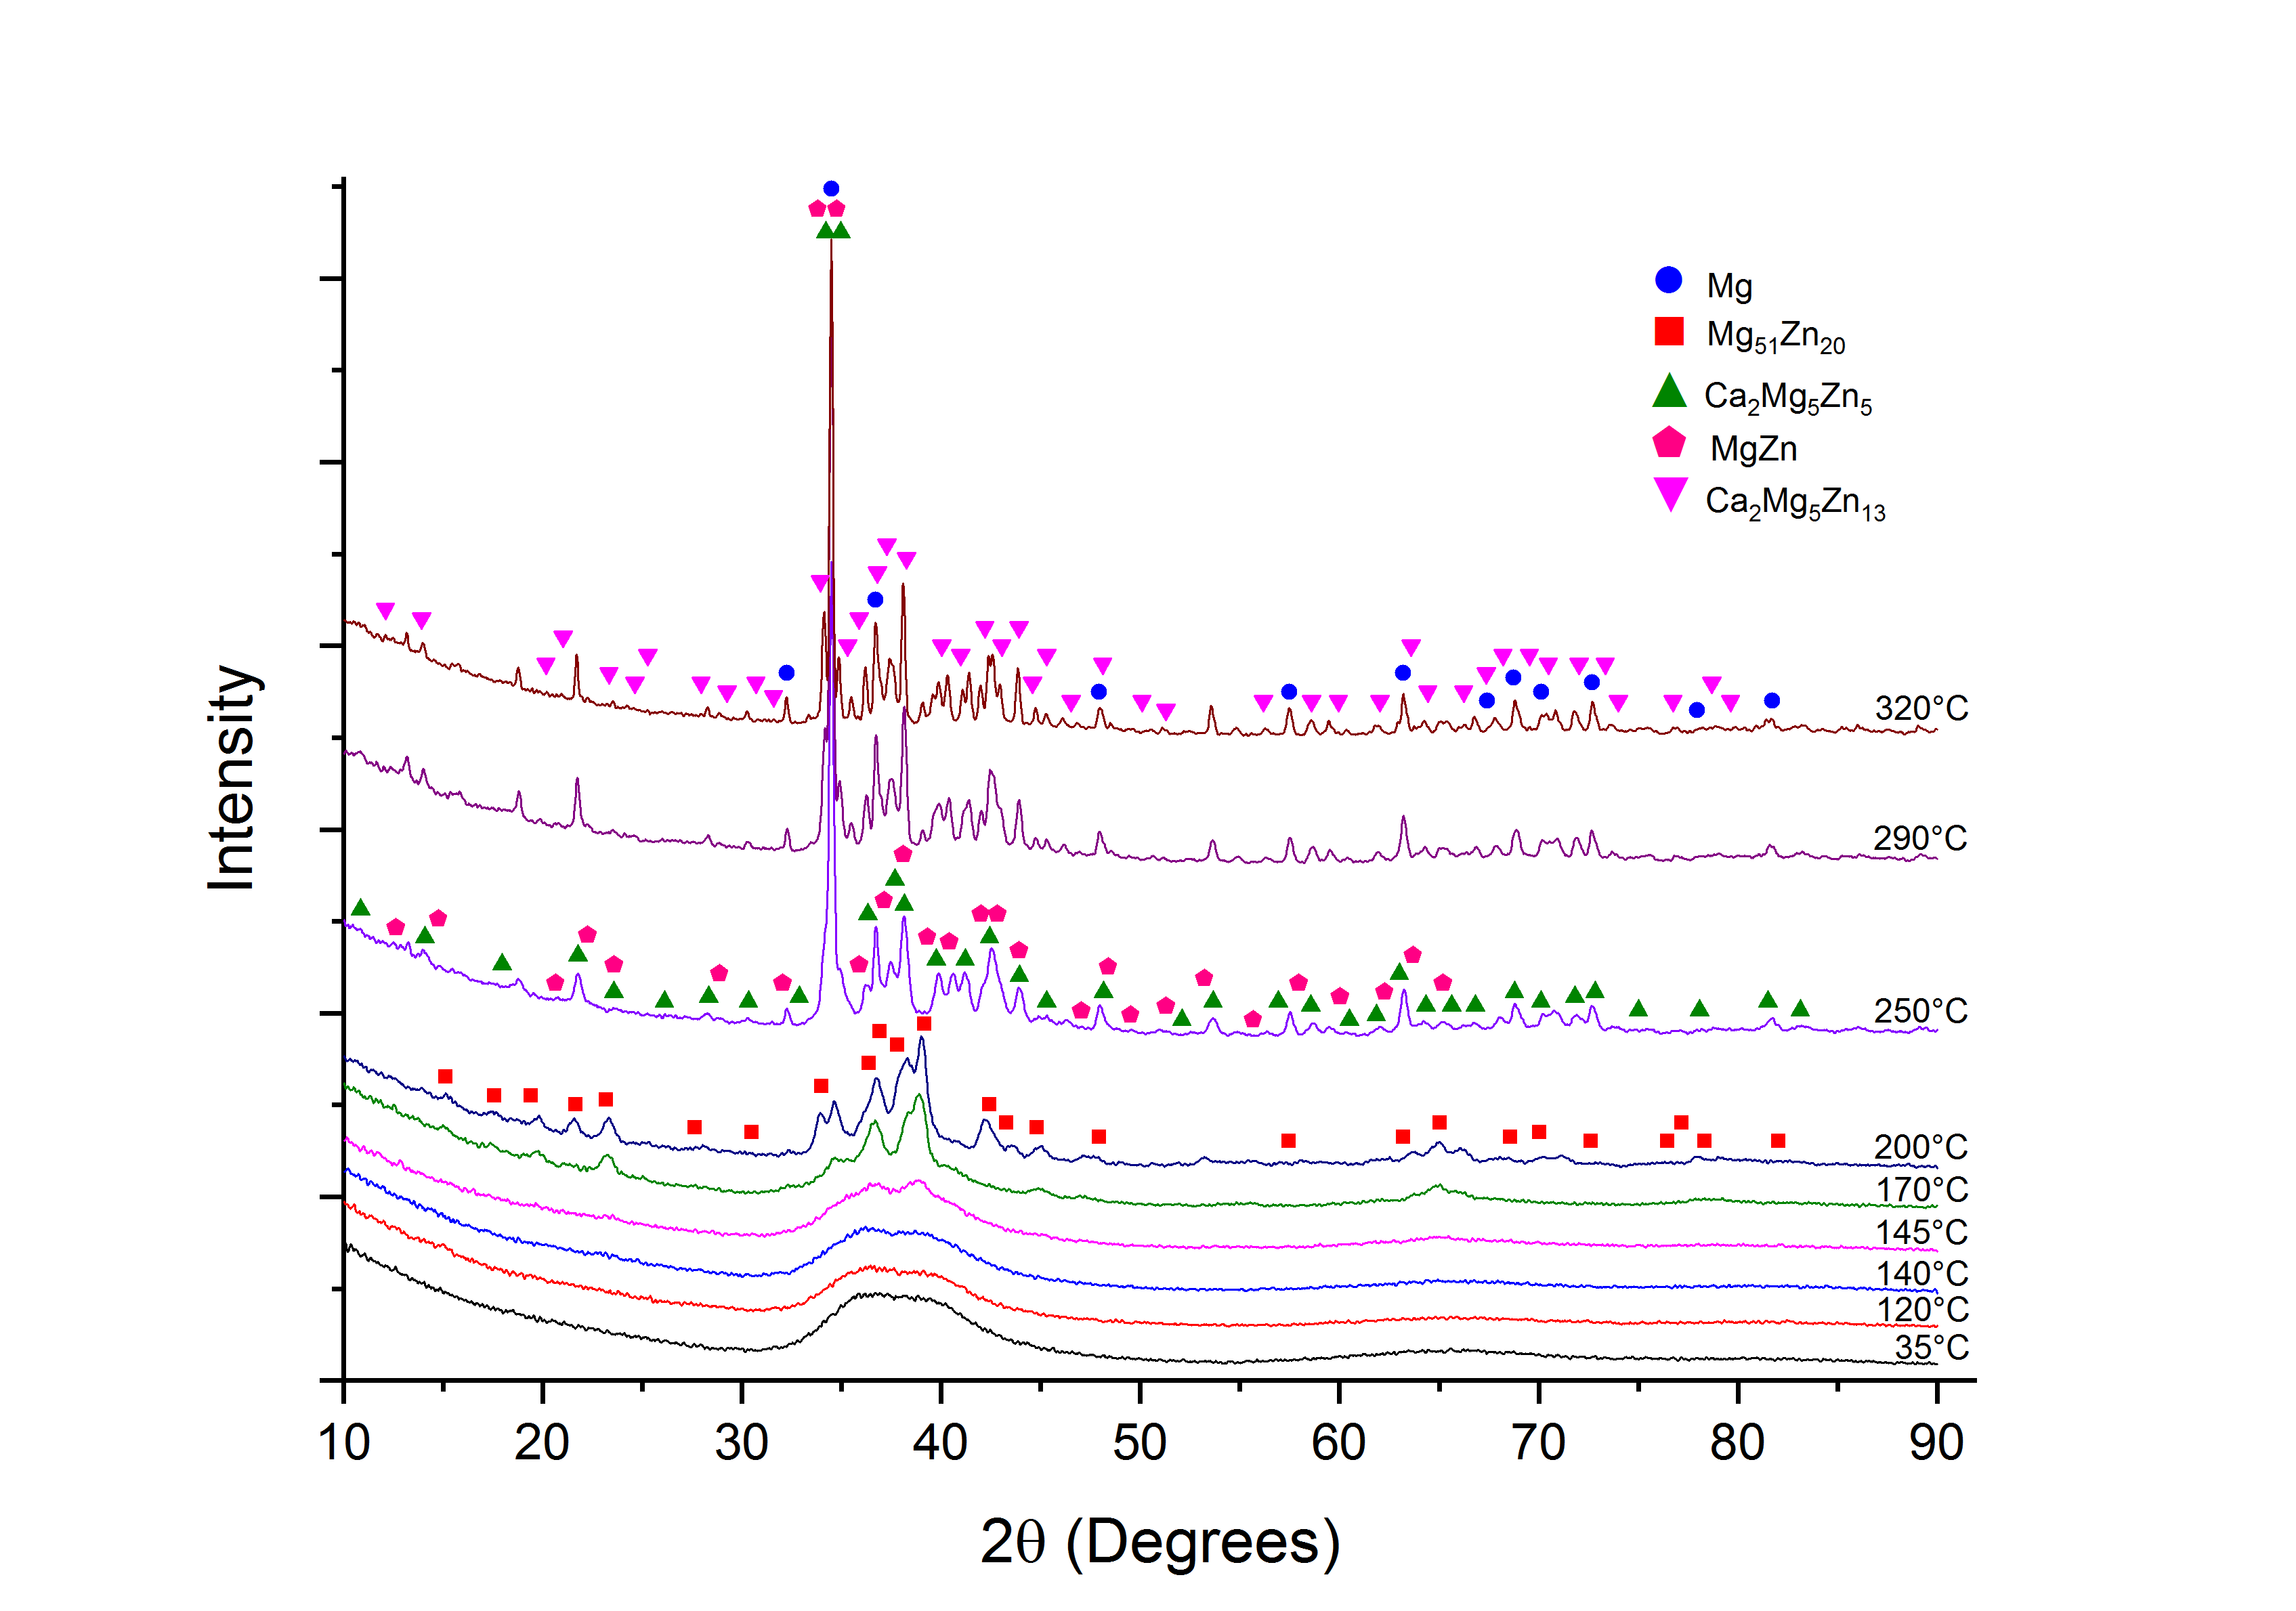
\includegraphics[width=0.85\textwidth]{XRD_Annealing_Bulk.png}
	\caption[Table of contents Capition]{\acrshort{xrd} pattern for bulk \MgZnCa~ heated treated to several temperatures for crystallisation peak identified from \acrshort{dsc}.}
	\label{fig:XRD_Annealing_Bulk}
\end{figure}

%single image
\begin{figure}[b]
	\centering
	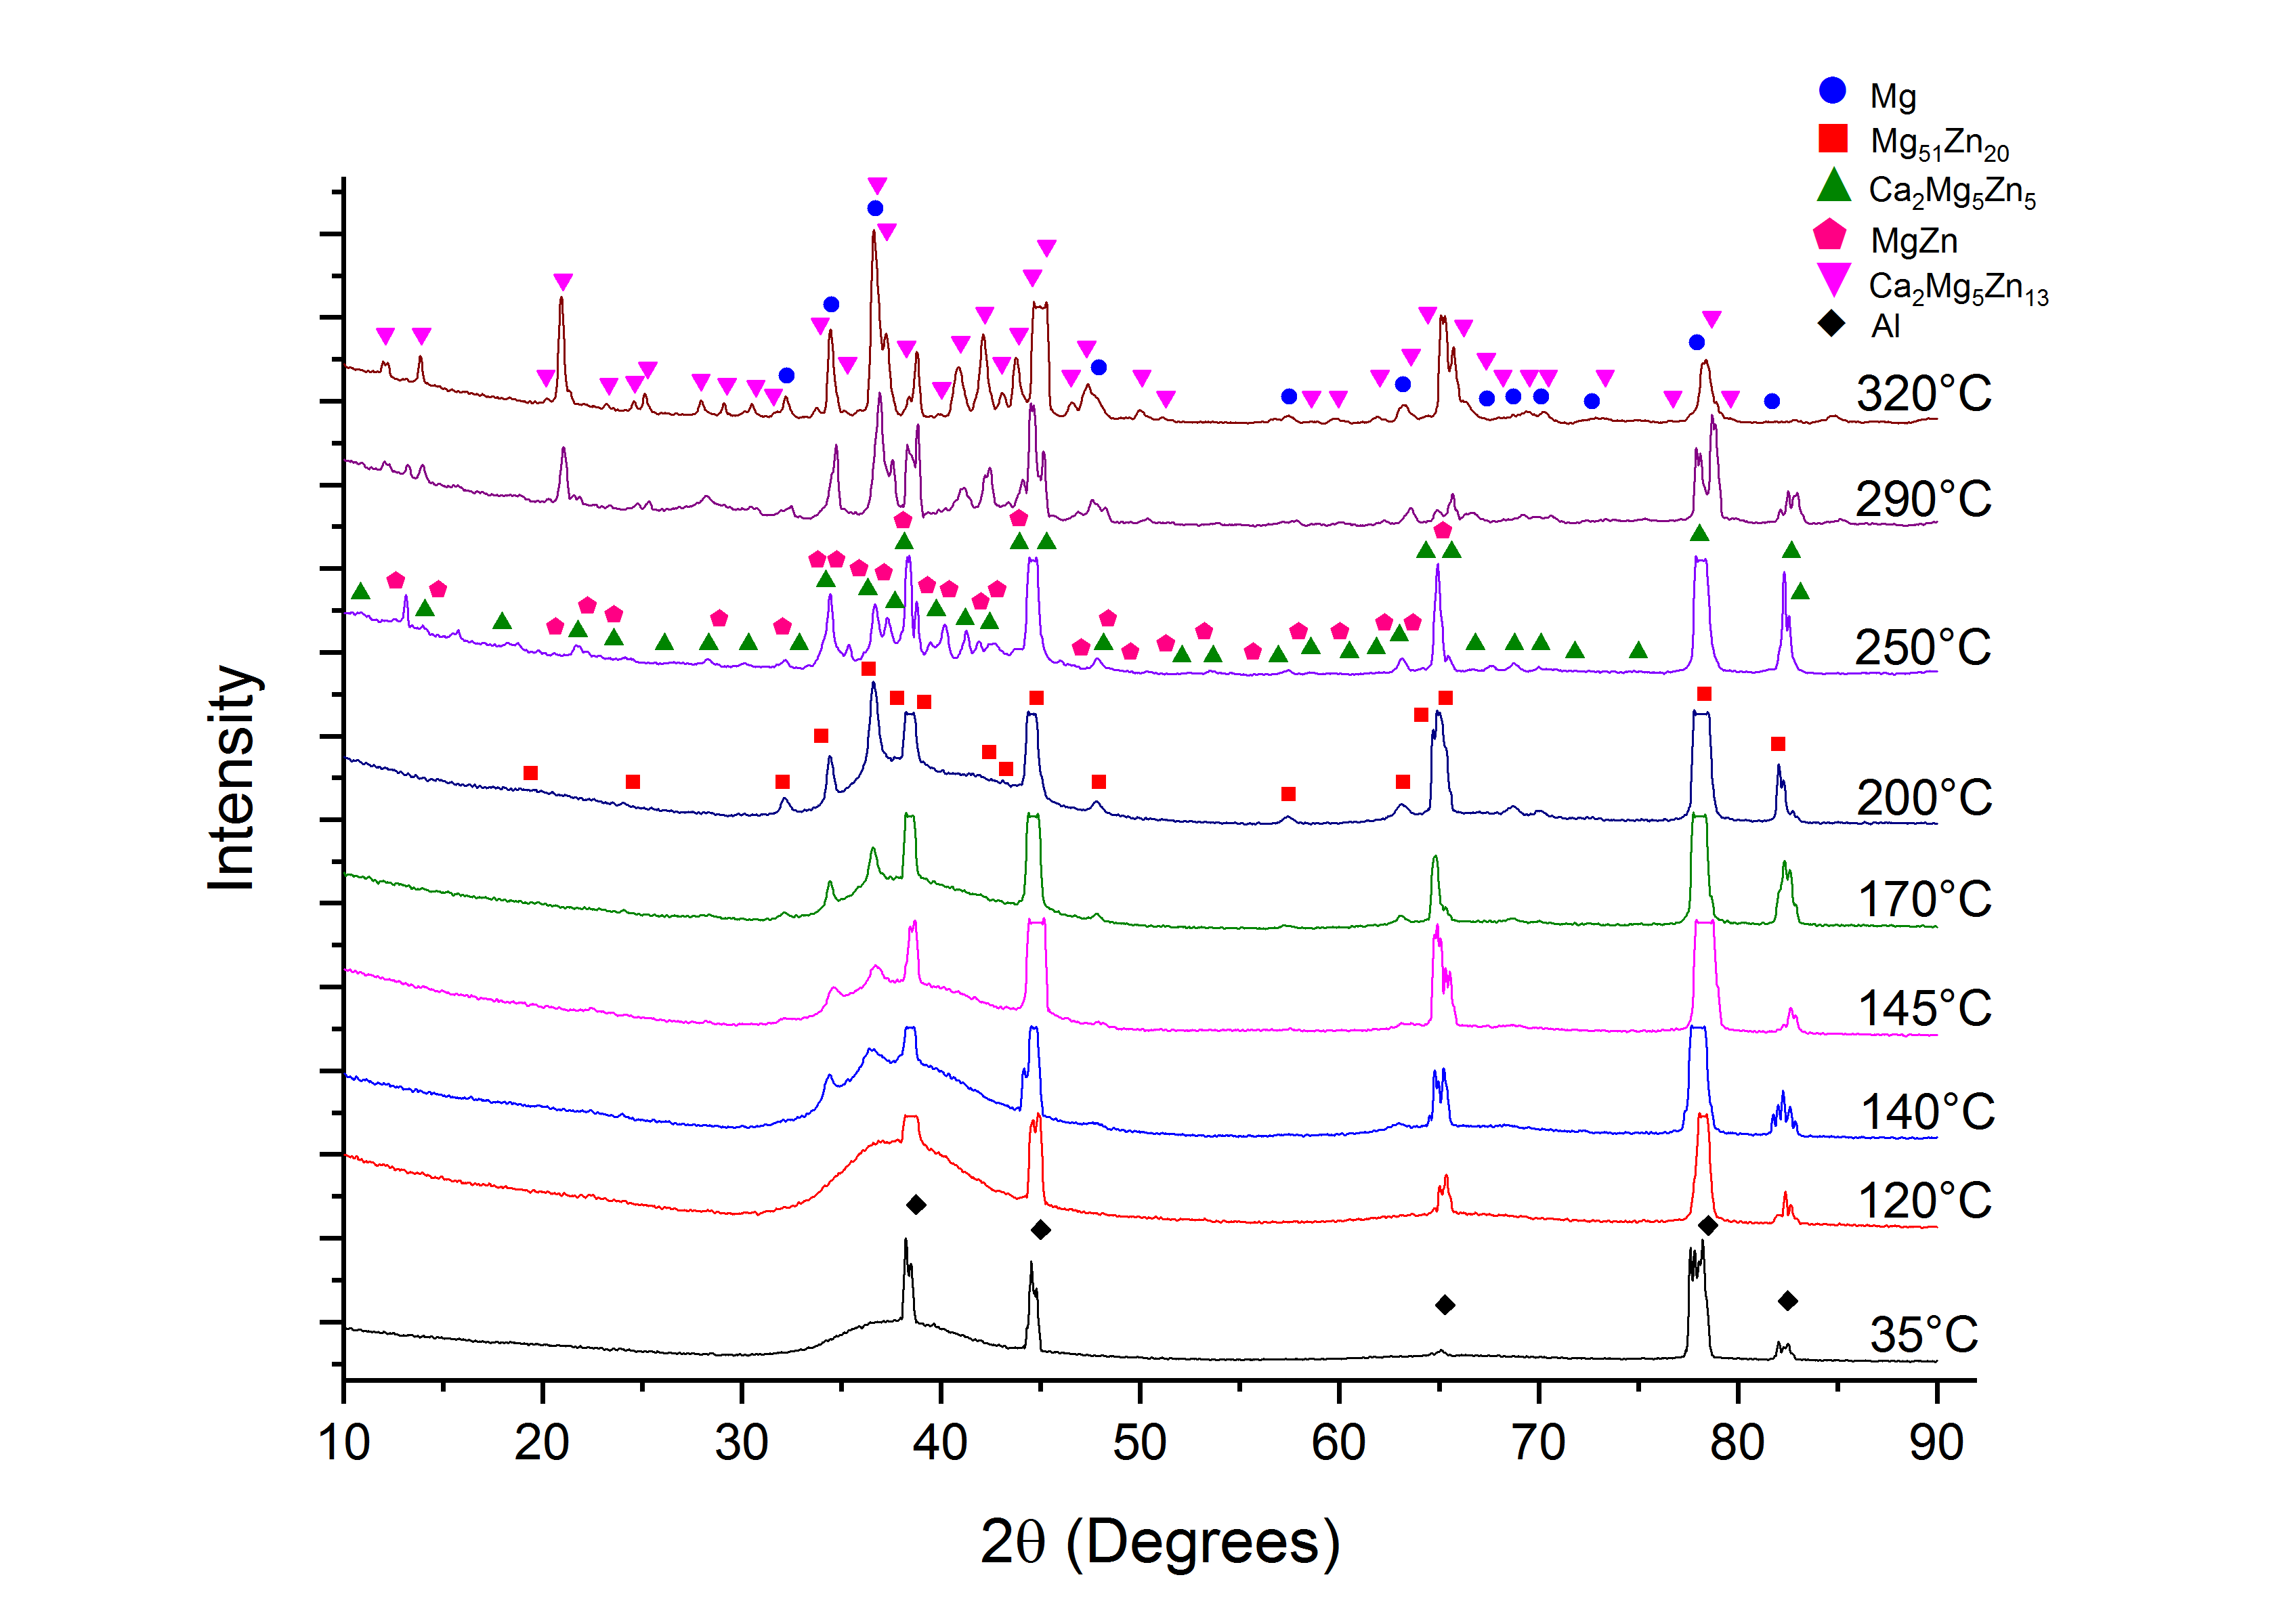
\includegraphics[width=0.85\textwidth]{XRD_Annealing_Film.png}
	\caption[Table of contents Capition]{\acrshort{xrd} pattern for film \MgZnCa~ heated treated to several temperatures for crystallisation peak identified from \acrshort{dsc}. Note the Al substrate peaks have been faceted as to not dwarf all other peaks.}
	\label{fig:XRD_Annealing_Film}
\end{figure}

\todo{peak shift can be seen in the annealing xrd. can make a table of that, but rates of nucleation is only seen in the dynamic.}

\subsubsection{Dynamic \acrshort{xrd}}

The annealing \acrshort{xrd} was useful for identifying the crystal phases present, but not many difference between the evolution rates of the bulk or film could be observed. Thus samples were subjected to dynamic \acrshort{xrd} over their most active $2 \theta$ range of $31-60$\degree~ to observe changes \textit{in-situ}. This allowed the crystallisation to be actively observed over the range of $35-185$\degree C, showing how phases evolved over time as the temperature was raised in 5\degree C increments. 

The dynamic \acrshort{xrd} data shows that many phases seen in the bulk nucleate at different temperatures, are not observed as strongly, or fail to nucleate in the film. The first Mg and \MgZn~ peak at 32.1\degree~ is first clearly seen in the bulk at a temperature of 170\degree C. In the film the first clear evidence of this peak is at 90\degree C, although its resolution is poor from 150-170\degree C. The Mg, \MgZn, and \CaMgZnFive~ peak at 34.3\degree~ is seen at 75\degree C in the bulk, but not till 115\degree C in the film. The Mg and \MgZn~ peak at 47.7\degree~ is seen in both the bulk and film at 170\degree C. 

In the bulk a double peak at 38\degree~ and 39\degree~ begins to emerge at 125\degree C, phases which never evolve in the film. The bulk \CaMgZnFive~ peaks at 42.3\degree~ and 43.7\degree~ start to emerge at 165\degree C and 170\degree C respectively, but are never seen in the film. The small 57.2\degree~ peak at 170\degree C is also never seen in the film. A final faint peak at 53.3\degree is seen in the bulk at 175\degree C, but never in the film. These observations are tabulated in Table \ref{tab:Dynamic_XRD}. The bulk \acrshort{xrd} is shown in Figure \ref{fig:XRD_Dynamic_Bulk}, and the film in Figure \ref{fig:XRD_Dynamic_Film}. Normalised plots allowing for easy identification of differences between the bulk and film are shown in Figures \ref{fig:XRD_Dynamic_185}, \ref{fig:XRD_Dynamic_145}, and \ref{fig:XRD_Dynamic_105}.

\begin{table}[h]
	\centering
	\caption{Main dynamic \gls{xrd} peaks for both the bulk and the film. Data shows minor shifting for peaks 3 and 8, large start temperature differences for peaks 1 and 2, and failure of peaks $4-7$, 9, and 10 to nucleation in the film.}
	\begin{tabular}{ c c c c c c c c }
		\toprule
		Peak & Bulk & Film & Change & Bulk Start & Film Start & Change & Phases \\
		& $2\theta$ & $2\theta$ & \% & \degree C & \degree C & \% & at\% \\
		\midrule
		1    & 32.1 & 32.1 & 0.0\%  & 170 & 90 & -47.1\% & Mg, \MgZn \\
		2    & 34.3 & 34.3 & 0.0\%  & 75  & 115 & 53.3\% & Mg, \MgZn, \CaMgZnFive \\
		3    & 36.6 & 36.5 & -0.3\% & 130 & 130 & 0.0\%  & Mg, \MgZn \\
		4    & 38.0 & N/A  & N/A    & 125 & N/A & N/A    & \MgZn, \CaMgZnFive \\
		5    & 39.0 & N/A  & N/A    & 125 & N/A & N/A    & \MgZn \\
		6    & 42.3 & N/A  & N/A    & 165 & N/A & N/A    & \CaMgZnFive \\
		7    & 43.7 & N/A  & N/A    & 170 & N/A & N/A    & \CaMgZnFive \\
		8    & 47.7 & 47.6 & -0.2\% & 170 & 170 & 0.0\%  & Mg, \MgZn \\
		9    & 53.3 & N/A  & N/A    & 175 & N/A & N/A    & \MgZn, \CaMgZnFive \\
		10   & 57.2 & N/A  & N/A    & 170 & N/A  & N/A   & Mg, \MgZn \\
		\bottomrule
	\end{tabular}
	\label{tab:Dynamic_XRD}
\end{table}

\begin{table}[h]
	\centering
	\caption{Location of the bulk and film peaks for the dynamic \acrshort{xrd} Mg, \MgZn, and \CaMgZnFive~ compounds.}
	\begin{tabular}{ c c c c c c c c c }
		\toprule
		\multicolumn{3}{c}{Mg} & \multicolumn{3}{c}{\MgZn} & \multicolumn{3}{c}{\CaMgZnFive} \\
		Bulk & Film & Change \% & Bulk & Film & Change \% & Bulk & Film & Change \% \\
		\midrule
		32.1 & 32.1 & 0.0\%  & 32.1 & 32.1   & 0.0\%  & 34.1 & 34.1 & 0.0\% \\
		34.3 & 34.3 & 0.0\%  & 34.3 & 34.3   & 0.0\%  & 34.6 & 35.1 & 1.4\% \\
		36.6 & 36.5 & -0.3\% & 36.6 & 36.5   & -0.3\% & 36.0 & 35.7 & -0.8\% \\
		47.7 & 47.6 & -0.2\% & 38.0 & 38.2   & 0.5\%  & 38.0 & 38.2 & 0.5\% \\
		57.2 & 57.1 & -0.2\% & 39.1 & 39.5   & 1.0\%  & 42.3 & 42.2 & -0.2\% \\
		&    &      & 45.1   & 45.2 & 0.2\%  & 43.7   & 43.3 & -0.9\% \\
		&    &      & 47.7   & 47.6 & -0.2\% & 53.3   & 53.0 & -0.6\% \\
		&    &      & 53.3   & 53.0 & -0.6\% &        &      &        \\
		&    &      & 57.2   & 57.1 & -0.2\% &        &      &        \\
		\bottomrule
	\end{tabular}
	\label{tab:Annealing_XRD_PeakShift}
\end{table}

%code to put 2 images side by side in a figure
\begin{figure}[b]
	\centering
	%Image 1
	\begin{subfigure}[htbp]{0.75\textwidth}
		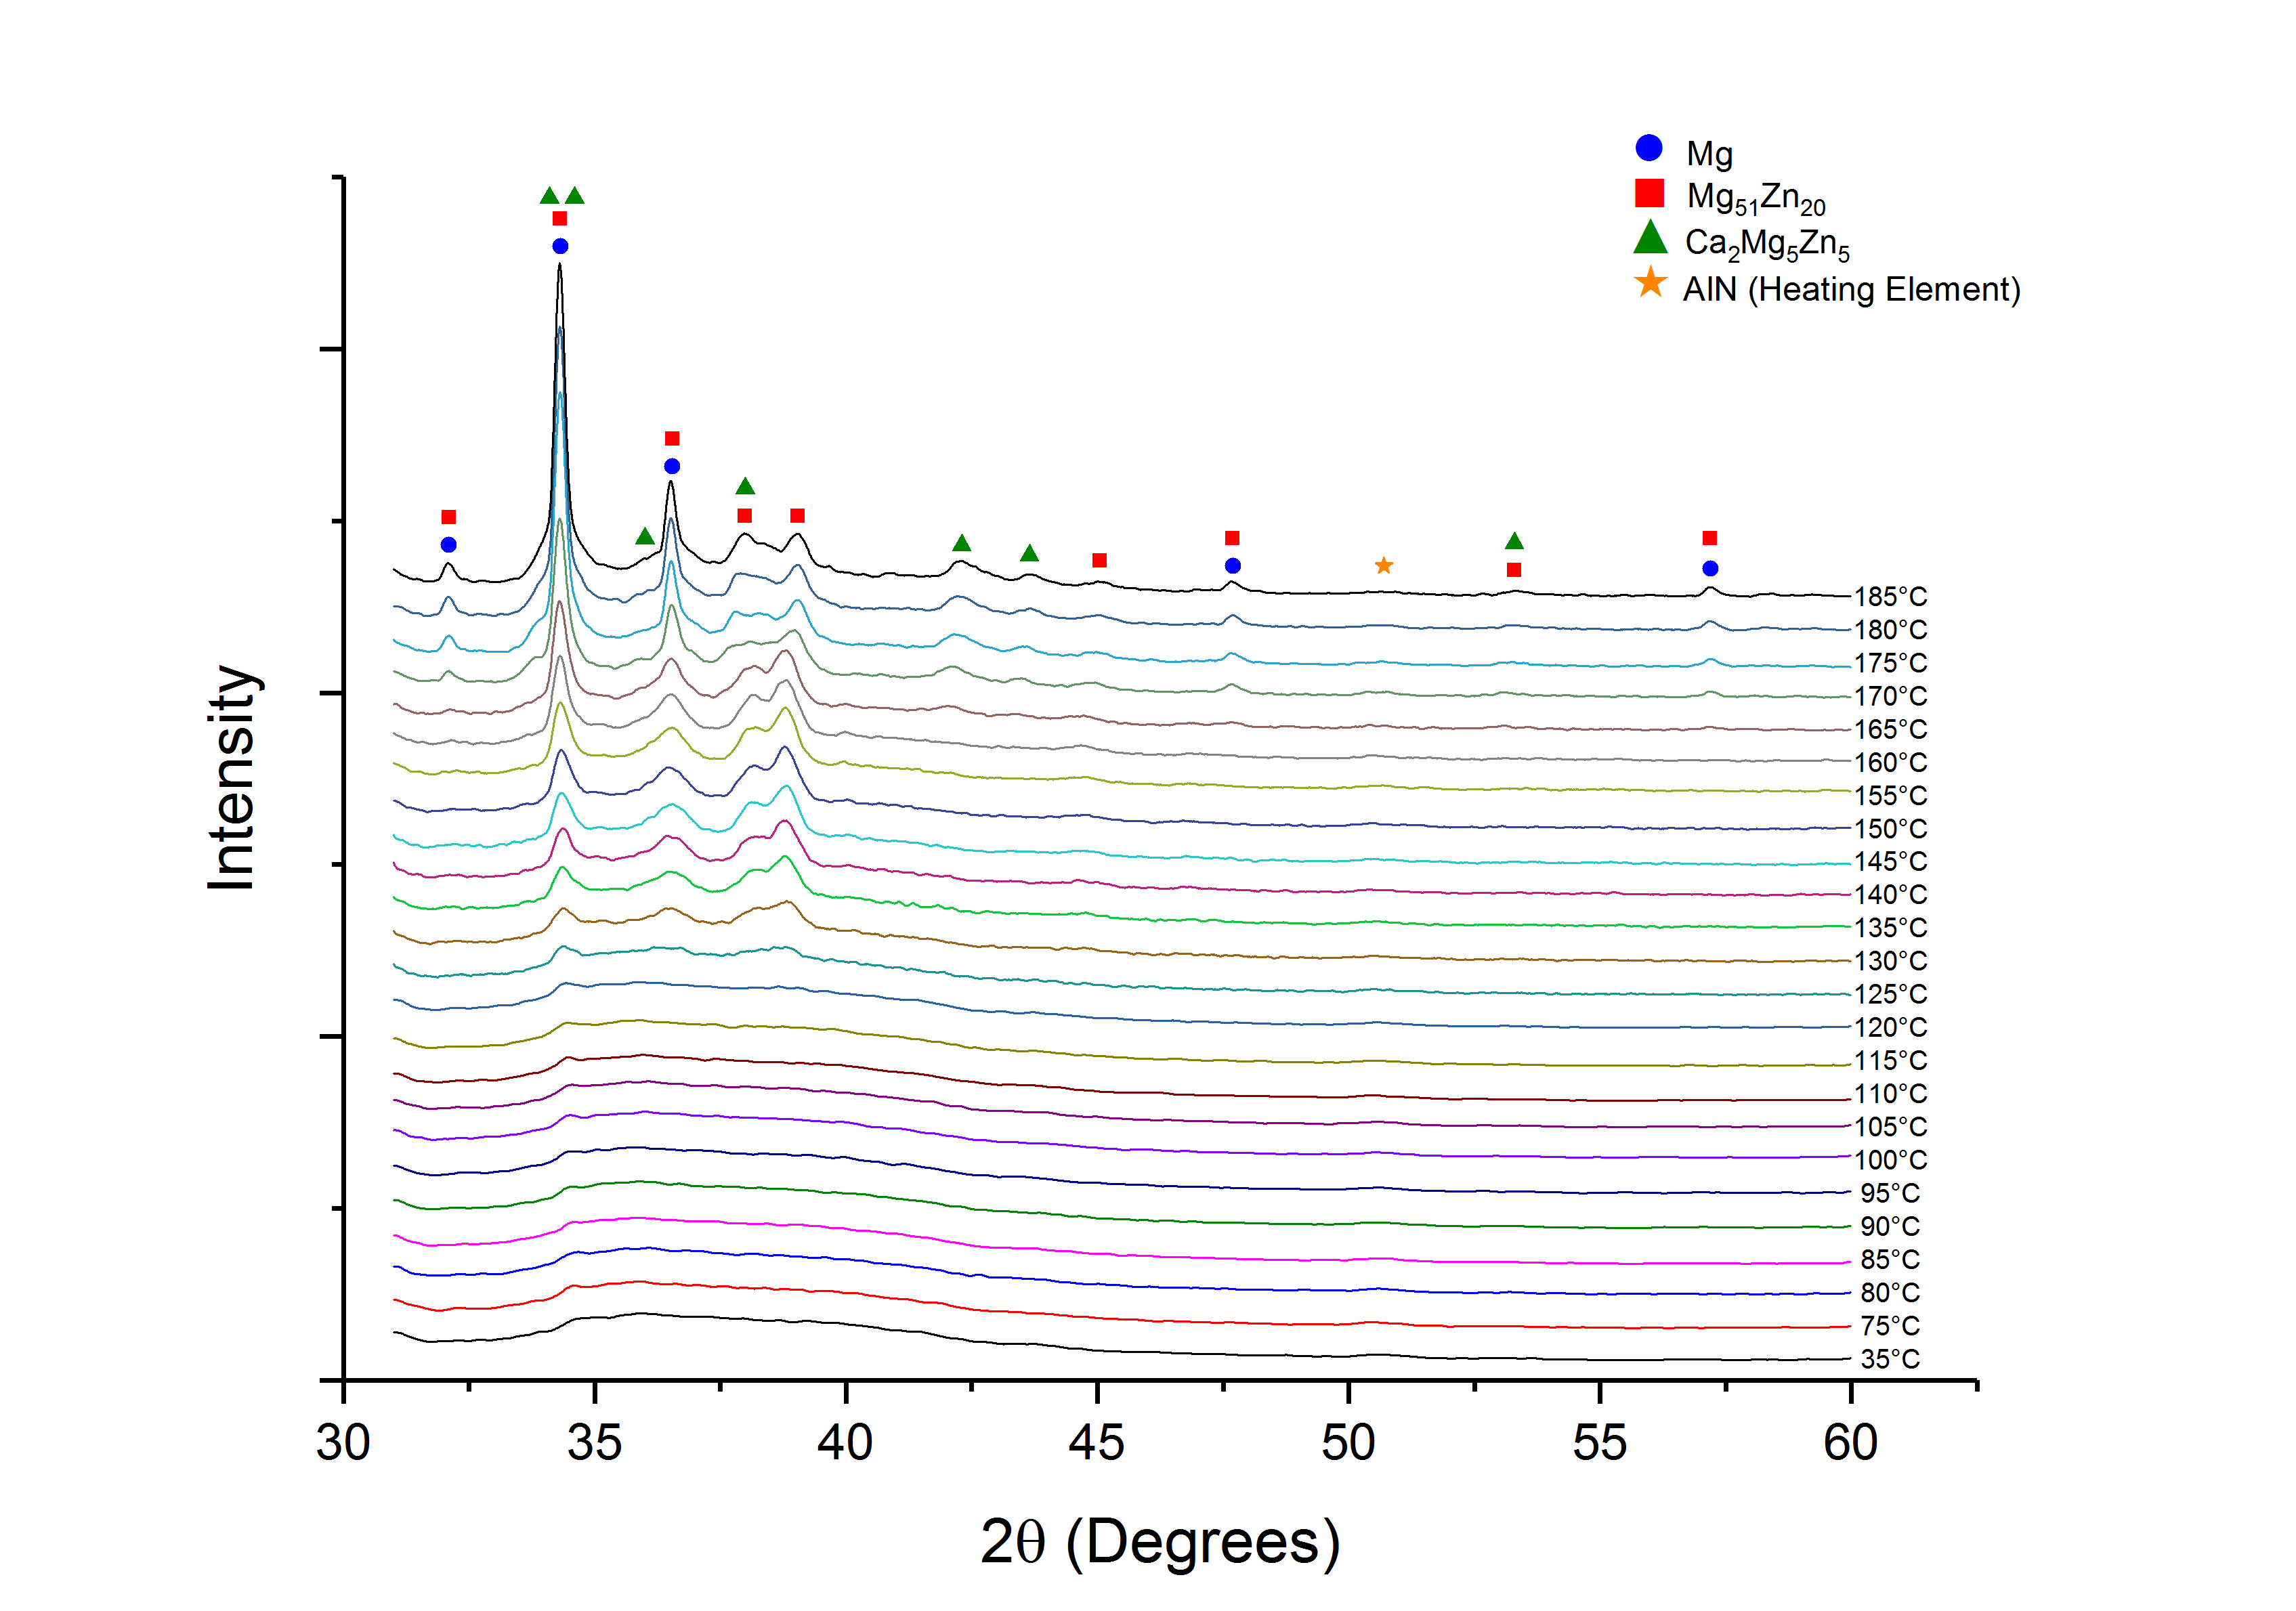
\includegraphics[width=\textwidth]{XRD_Dynamic_Bulk.png}
		\caption{}
		\label{fig:XRD_Dynamic_FullStack_Bulk}
	\end{subfigure}
	%Image 2
	\begin{subfigure}[htbp]{0.75\textwidth}
		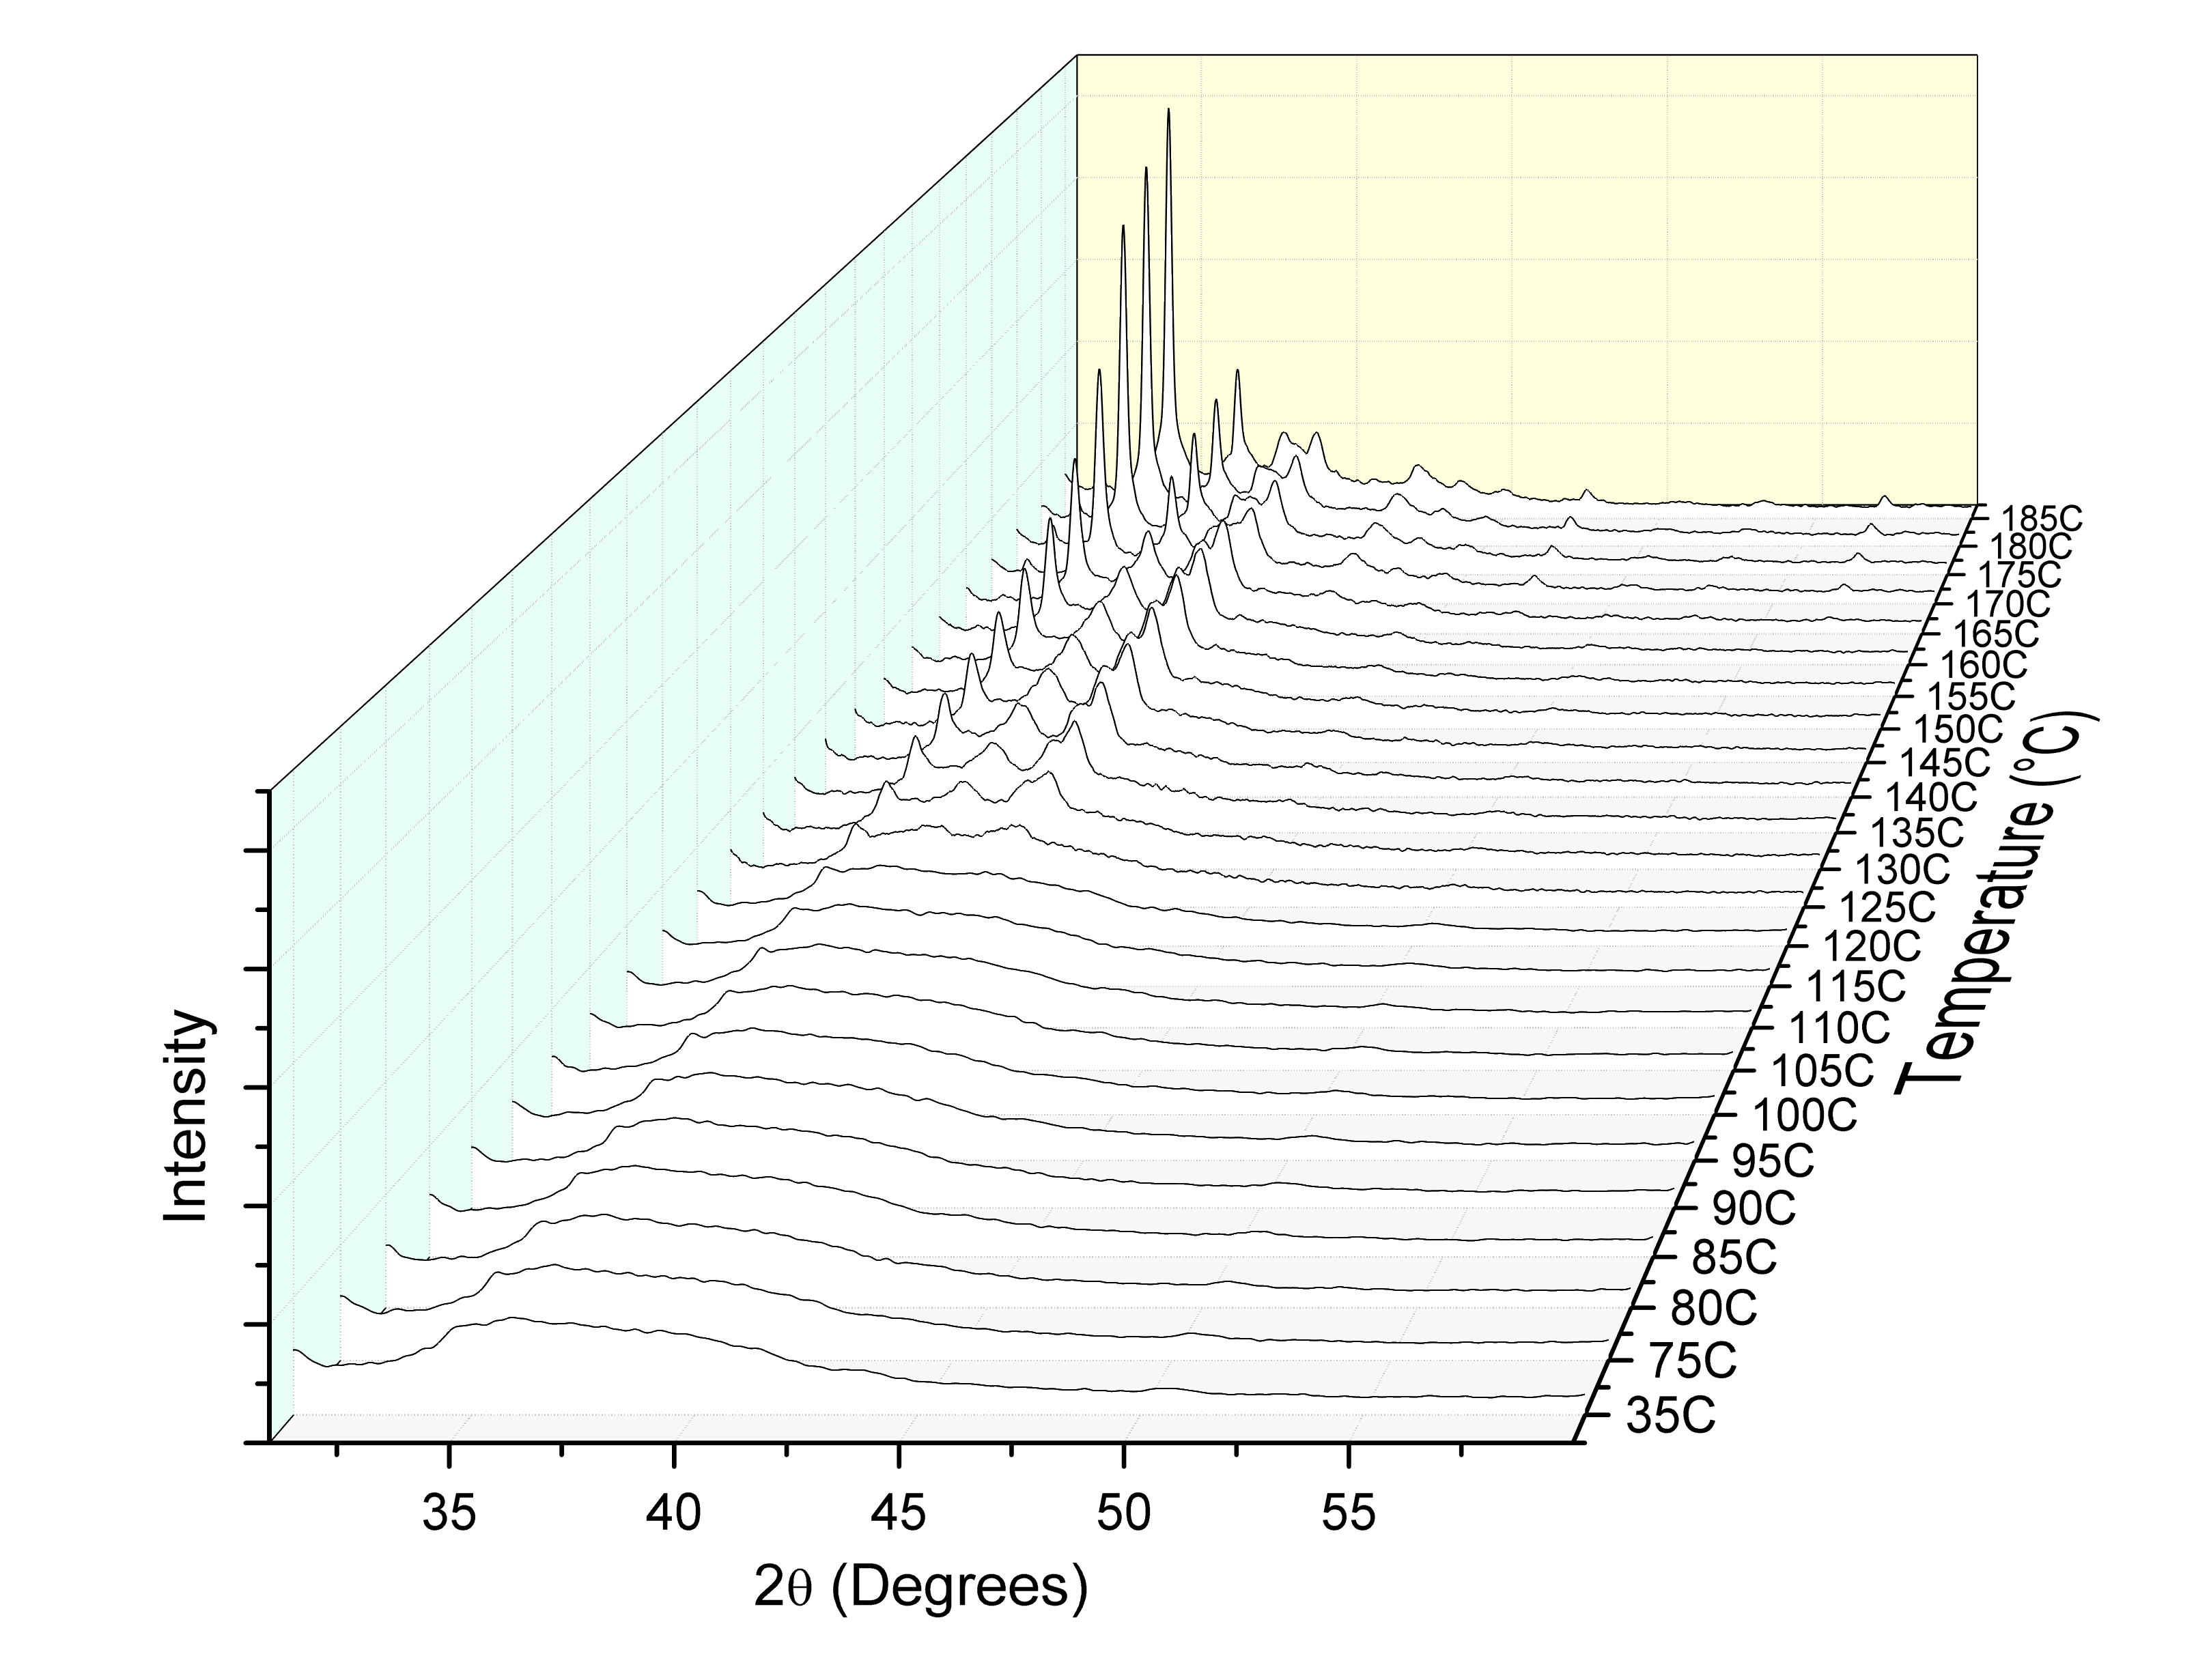
\includegraphics[width=\textwidth]{Bulk_Heated_XRD_Waterfall3D_Smooth2.png}
		\caption{}
		\label{fig:XRD_Dynamic_WaterFall_Bulk}
	\end{subfigure}
	\caption{(a) Stacked \acrshort{xrd} patterns from the incremental dynamic \textit{in-situ} heating of bulk \MgZnCa. Note the peak around $51$\degree~ is attributed to the AlN heating element. (b) The same \acrshort{xrd} patterns as (a) presented in a cascading layout.}%global caption
	\label{fig:XRD_Dynamic_Bulk}
\end{figure}

%code to put 2 images side by side in a figure
\begin{figure}[b]
	\centering
	%Image 1
	\begin{subfigure}[htbp]{0.75\textwidth}
		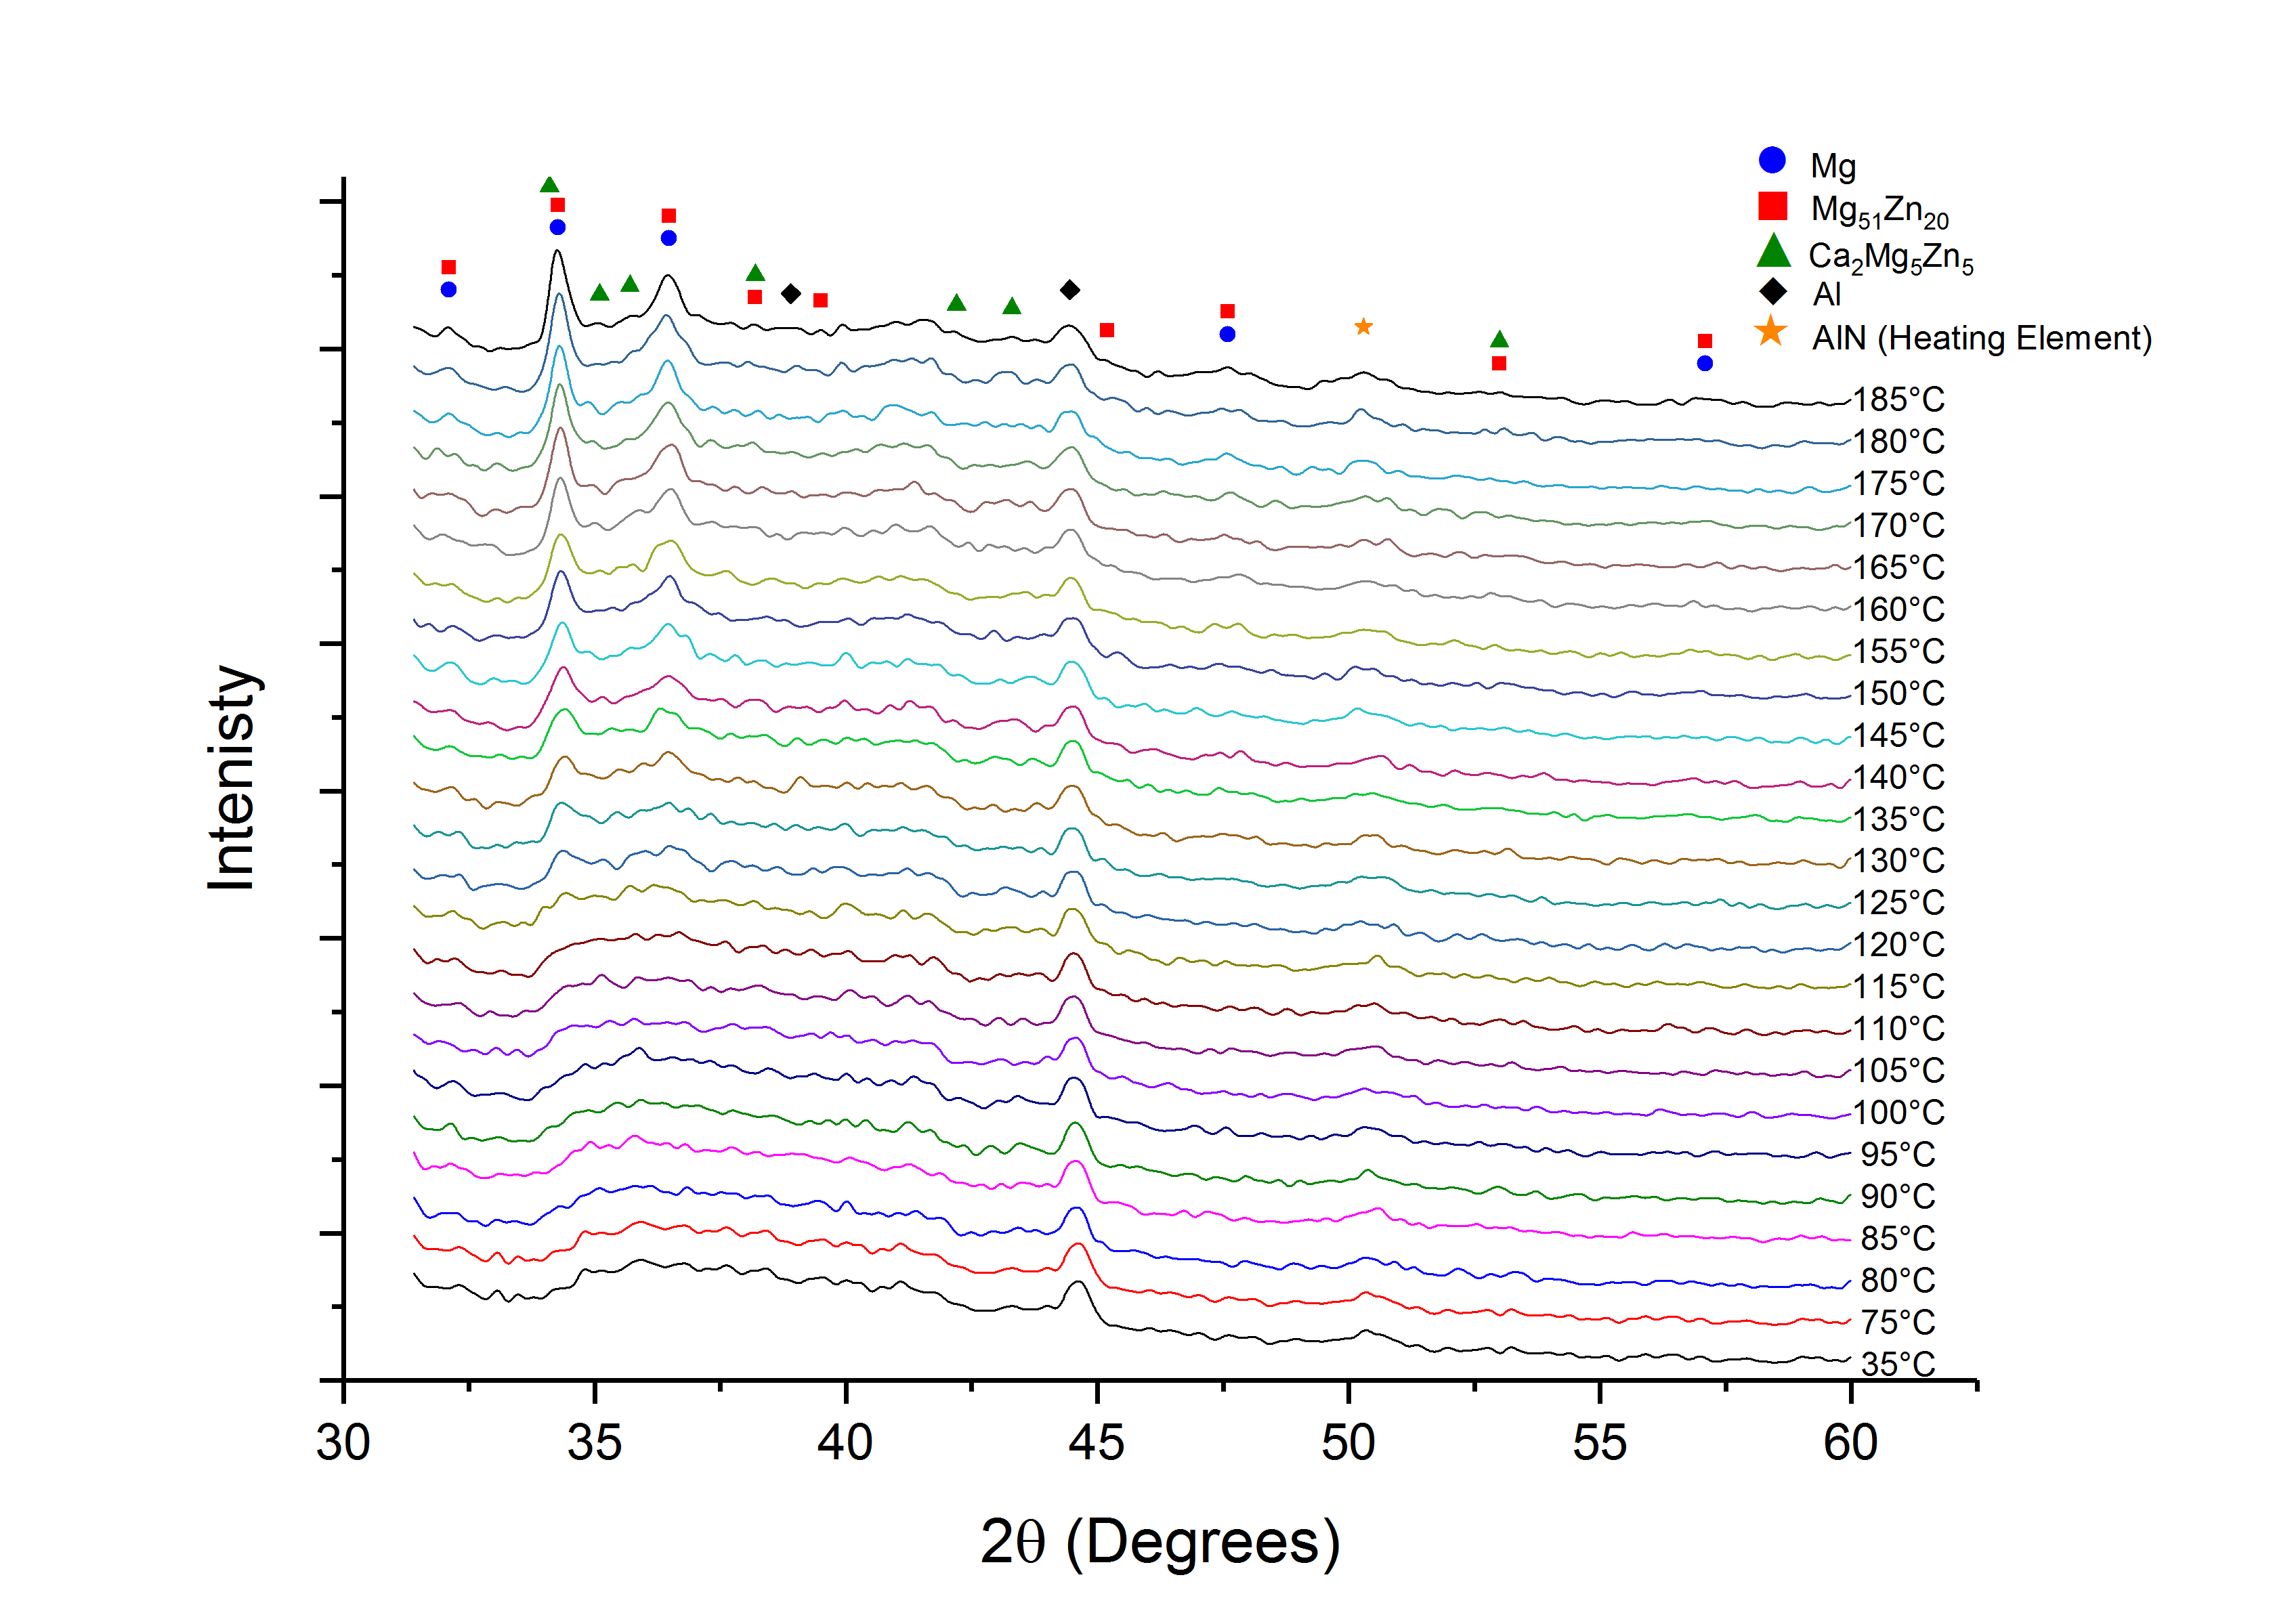
\includegraphics[width=\textwidth]{XRD_Dynamic_Film.png}
		\caption{}
		\label{fig:XRD_Dynamic_FullStack_Film}
	\end{subfigure}
	%Image 2
	\begin{subfigure}[htbp]{0.75\textwidth}
		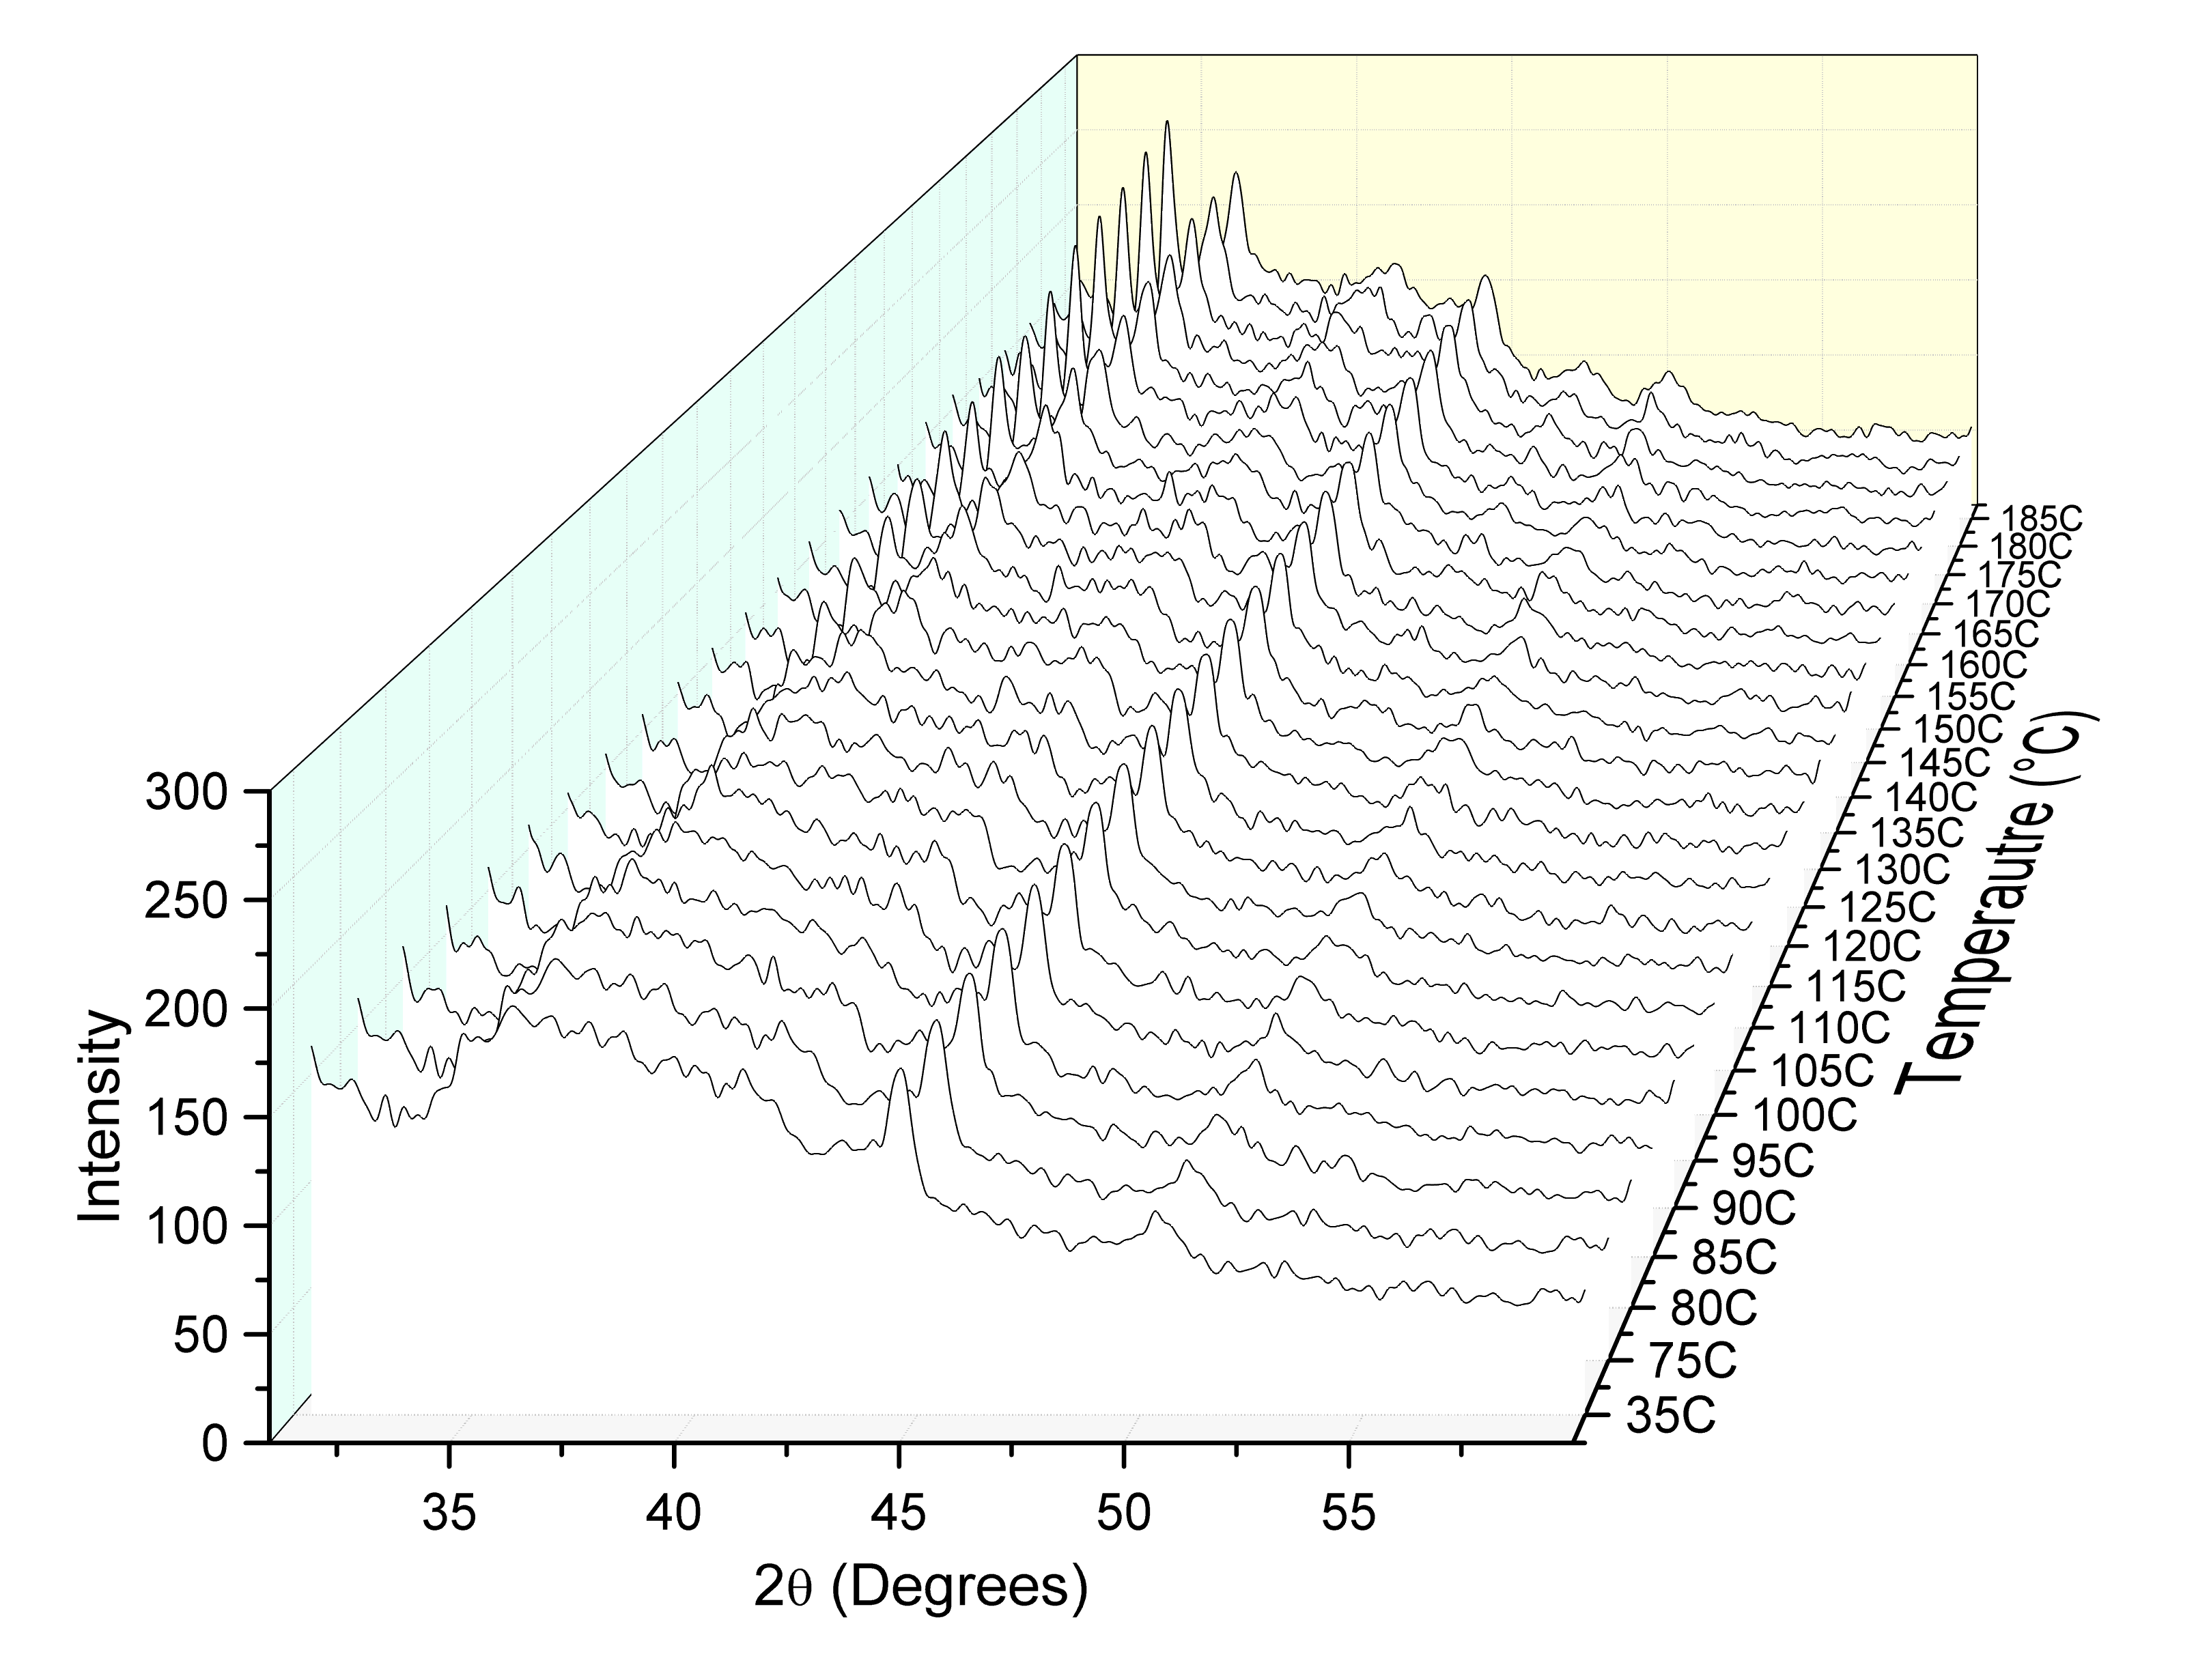
\includegraphics[width=\textwidth]{TF_Facet_HeatXRD_Waterfall3D_Smooth.png}
		\caption{}
		\label{fig:XRD_Dynamic_WaterFall_Film}
	\end{subfigure}
	\caption{(a) Stacked \acrshort{xrd} patterns from the incremental dynamic \textit{in-situ} heating of film \MgZnCa. Note the peak around $51$\degree~ is attributed to the AlN heating element, and the Al substrate peaks have been faceted as to not dwarf all other peaks. (b) The same \acrshort{xrd} patterns as (a) presented in a cascading layout.}%global caption
	\label{fig:XRD_Dynamic_Film}
\end{figure}

%single image
\begin{figure}[b]
	\centering
	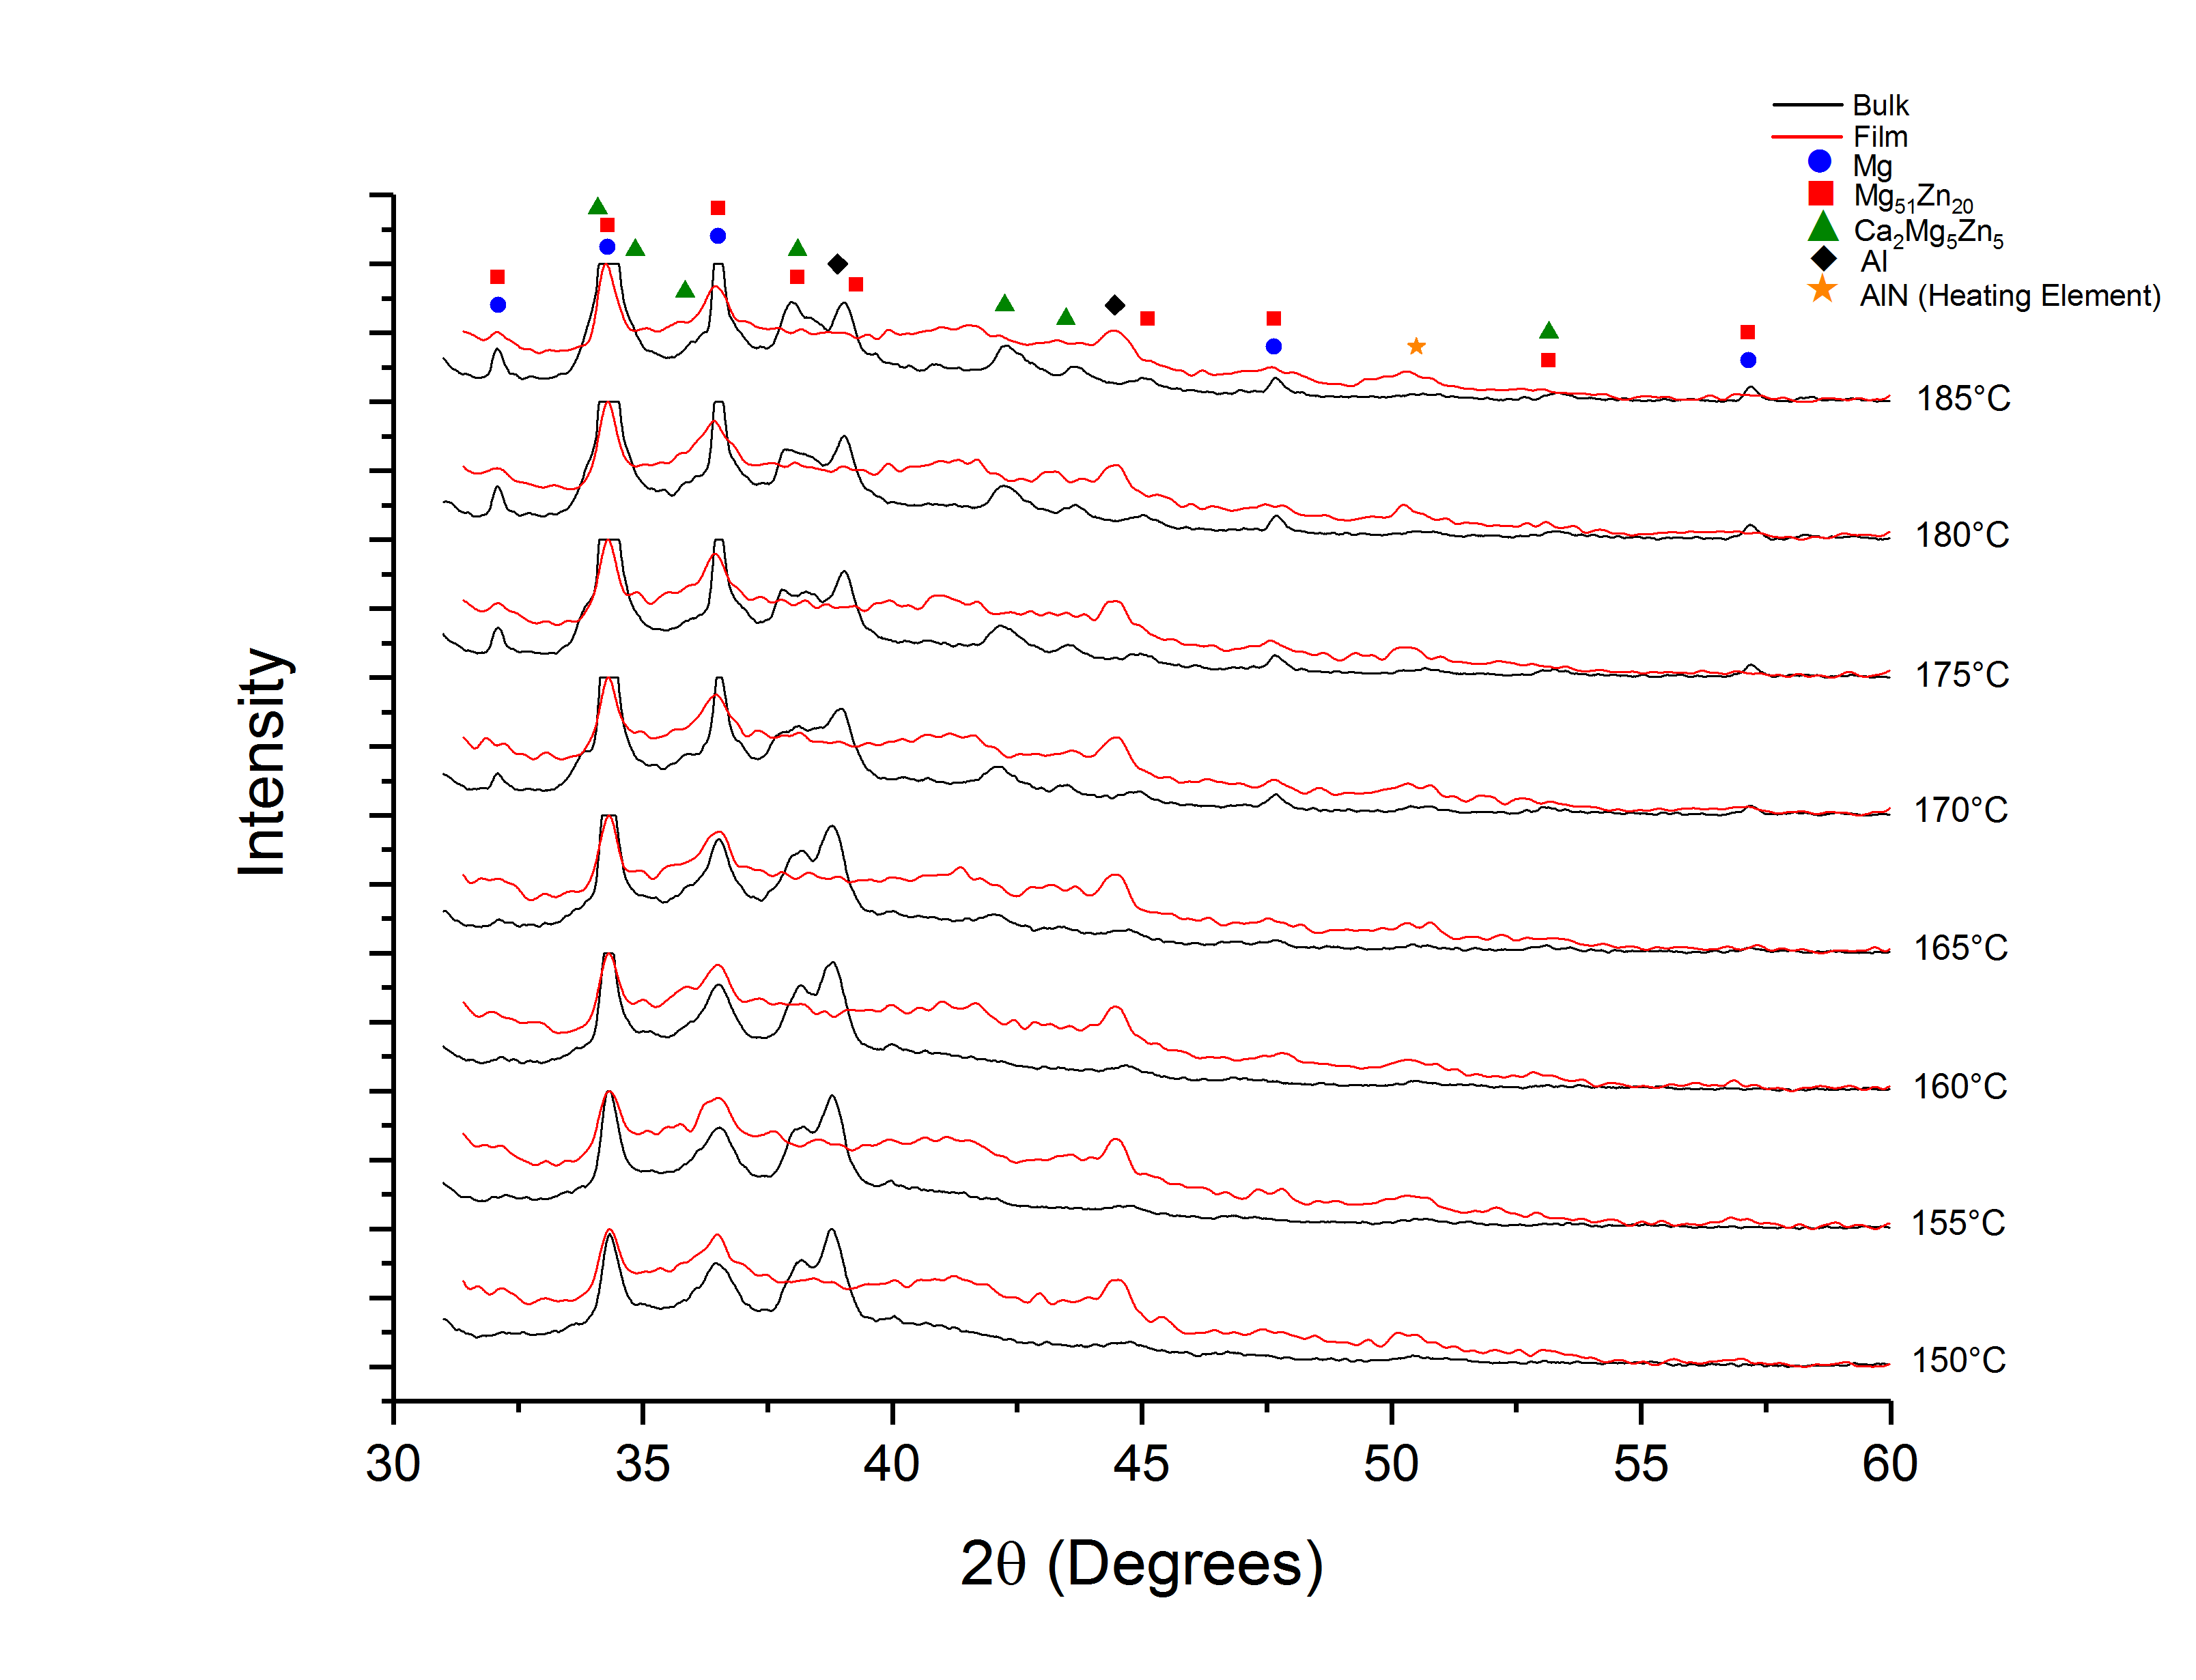
\includegraphics[width=0.85\textwidth]{XRD_Normalised_Dynamic_185.png}
	\caption[Table of contents Capition]{Normalised dynamic \acrshort{xrd} from $150-185$\degree C. Large bulk peaks have been faceted as to not dwarf smaller peaks and details.}%global caption
	\label{fig:XRD_Dynamic_185}
\end{figure}

%single image
\begin{figure}[b]
	\centering
	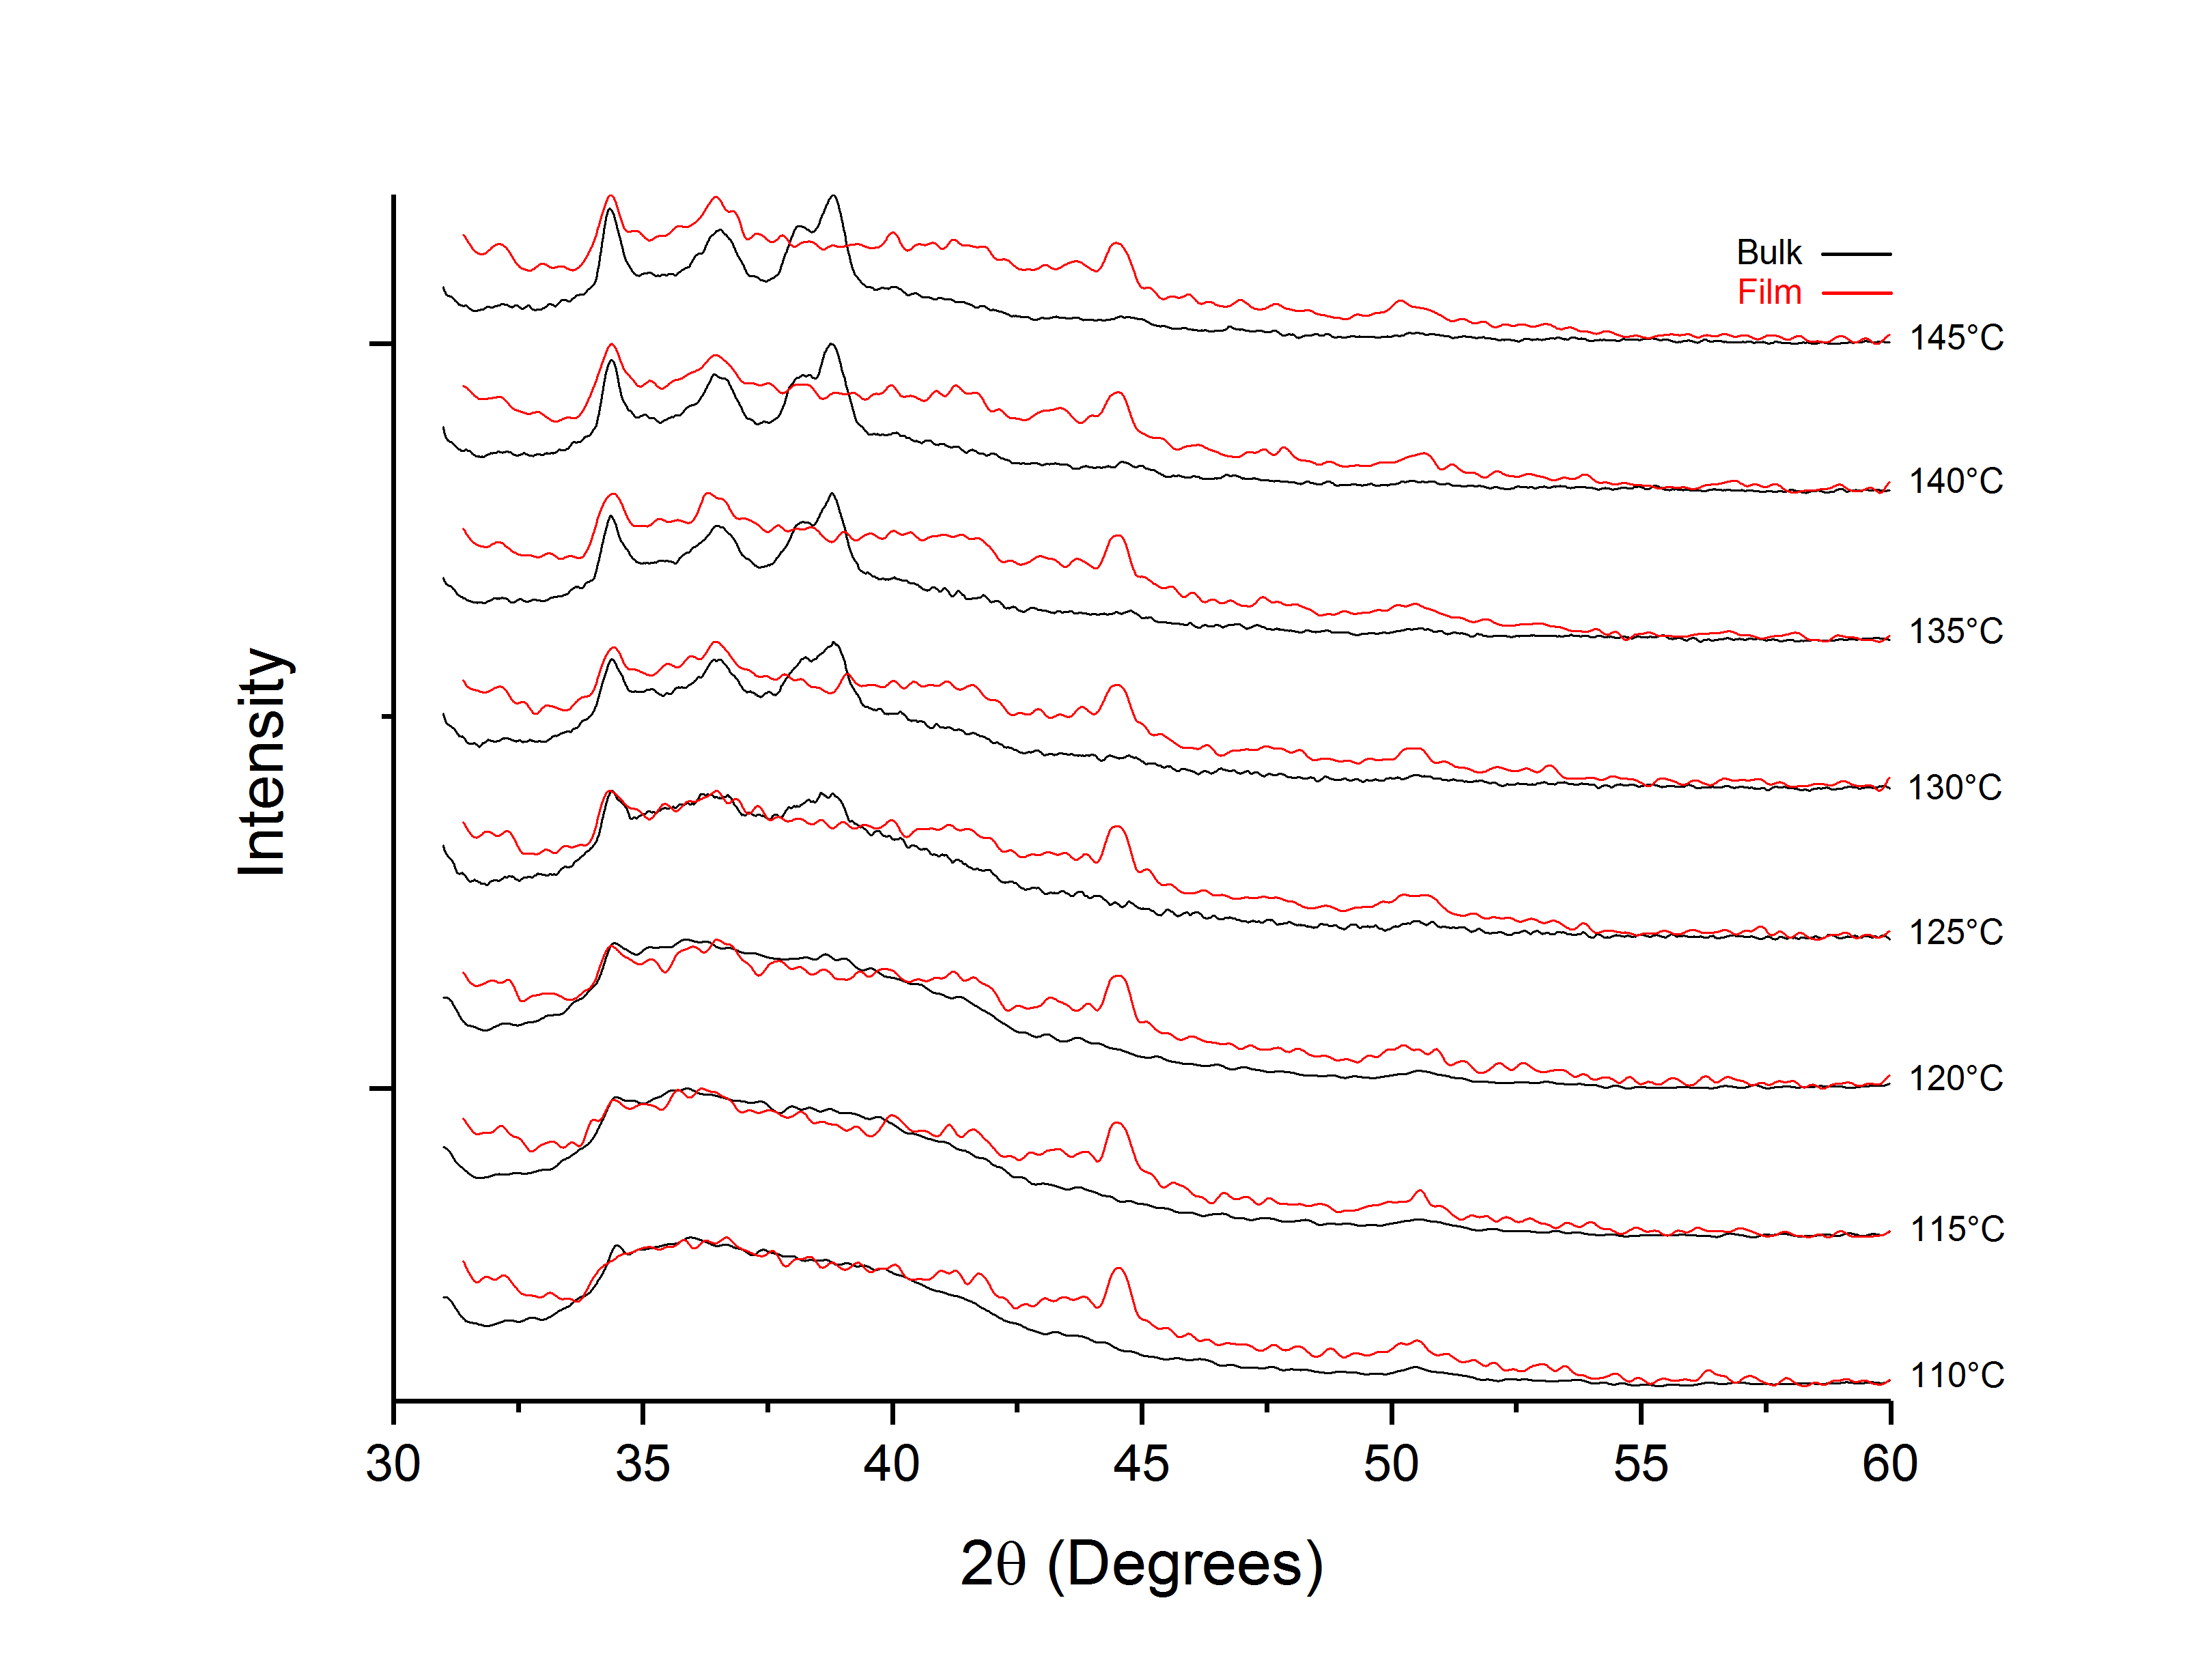
\includegraphics[width=0.85\textwidth]{XRD_Normalised_Dynamic_145.png}
	\caption[Table of contents Capition]{Normalised dynamic \acrshort{xrd} from $110-145$\degree C.}%global caption
	\label{fig:XRD_Dynamic_145}
\end{figure}

%single image
\begin{figure}[b]
	\centering
	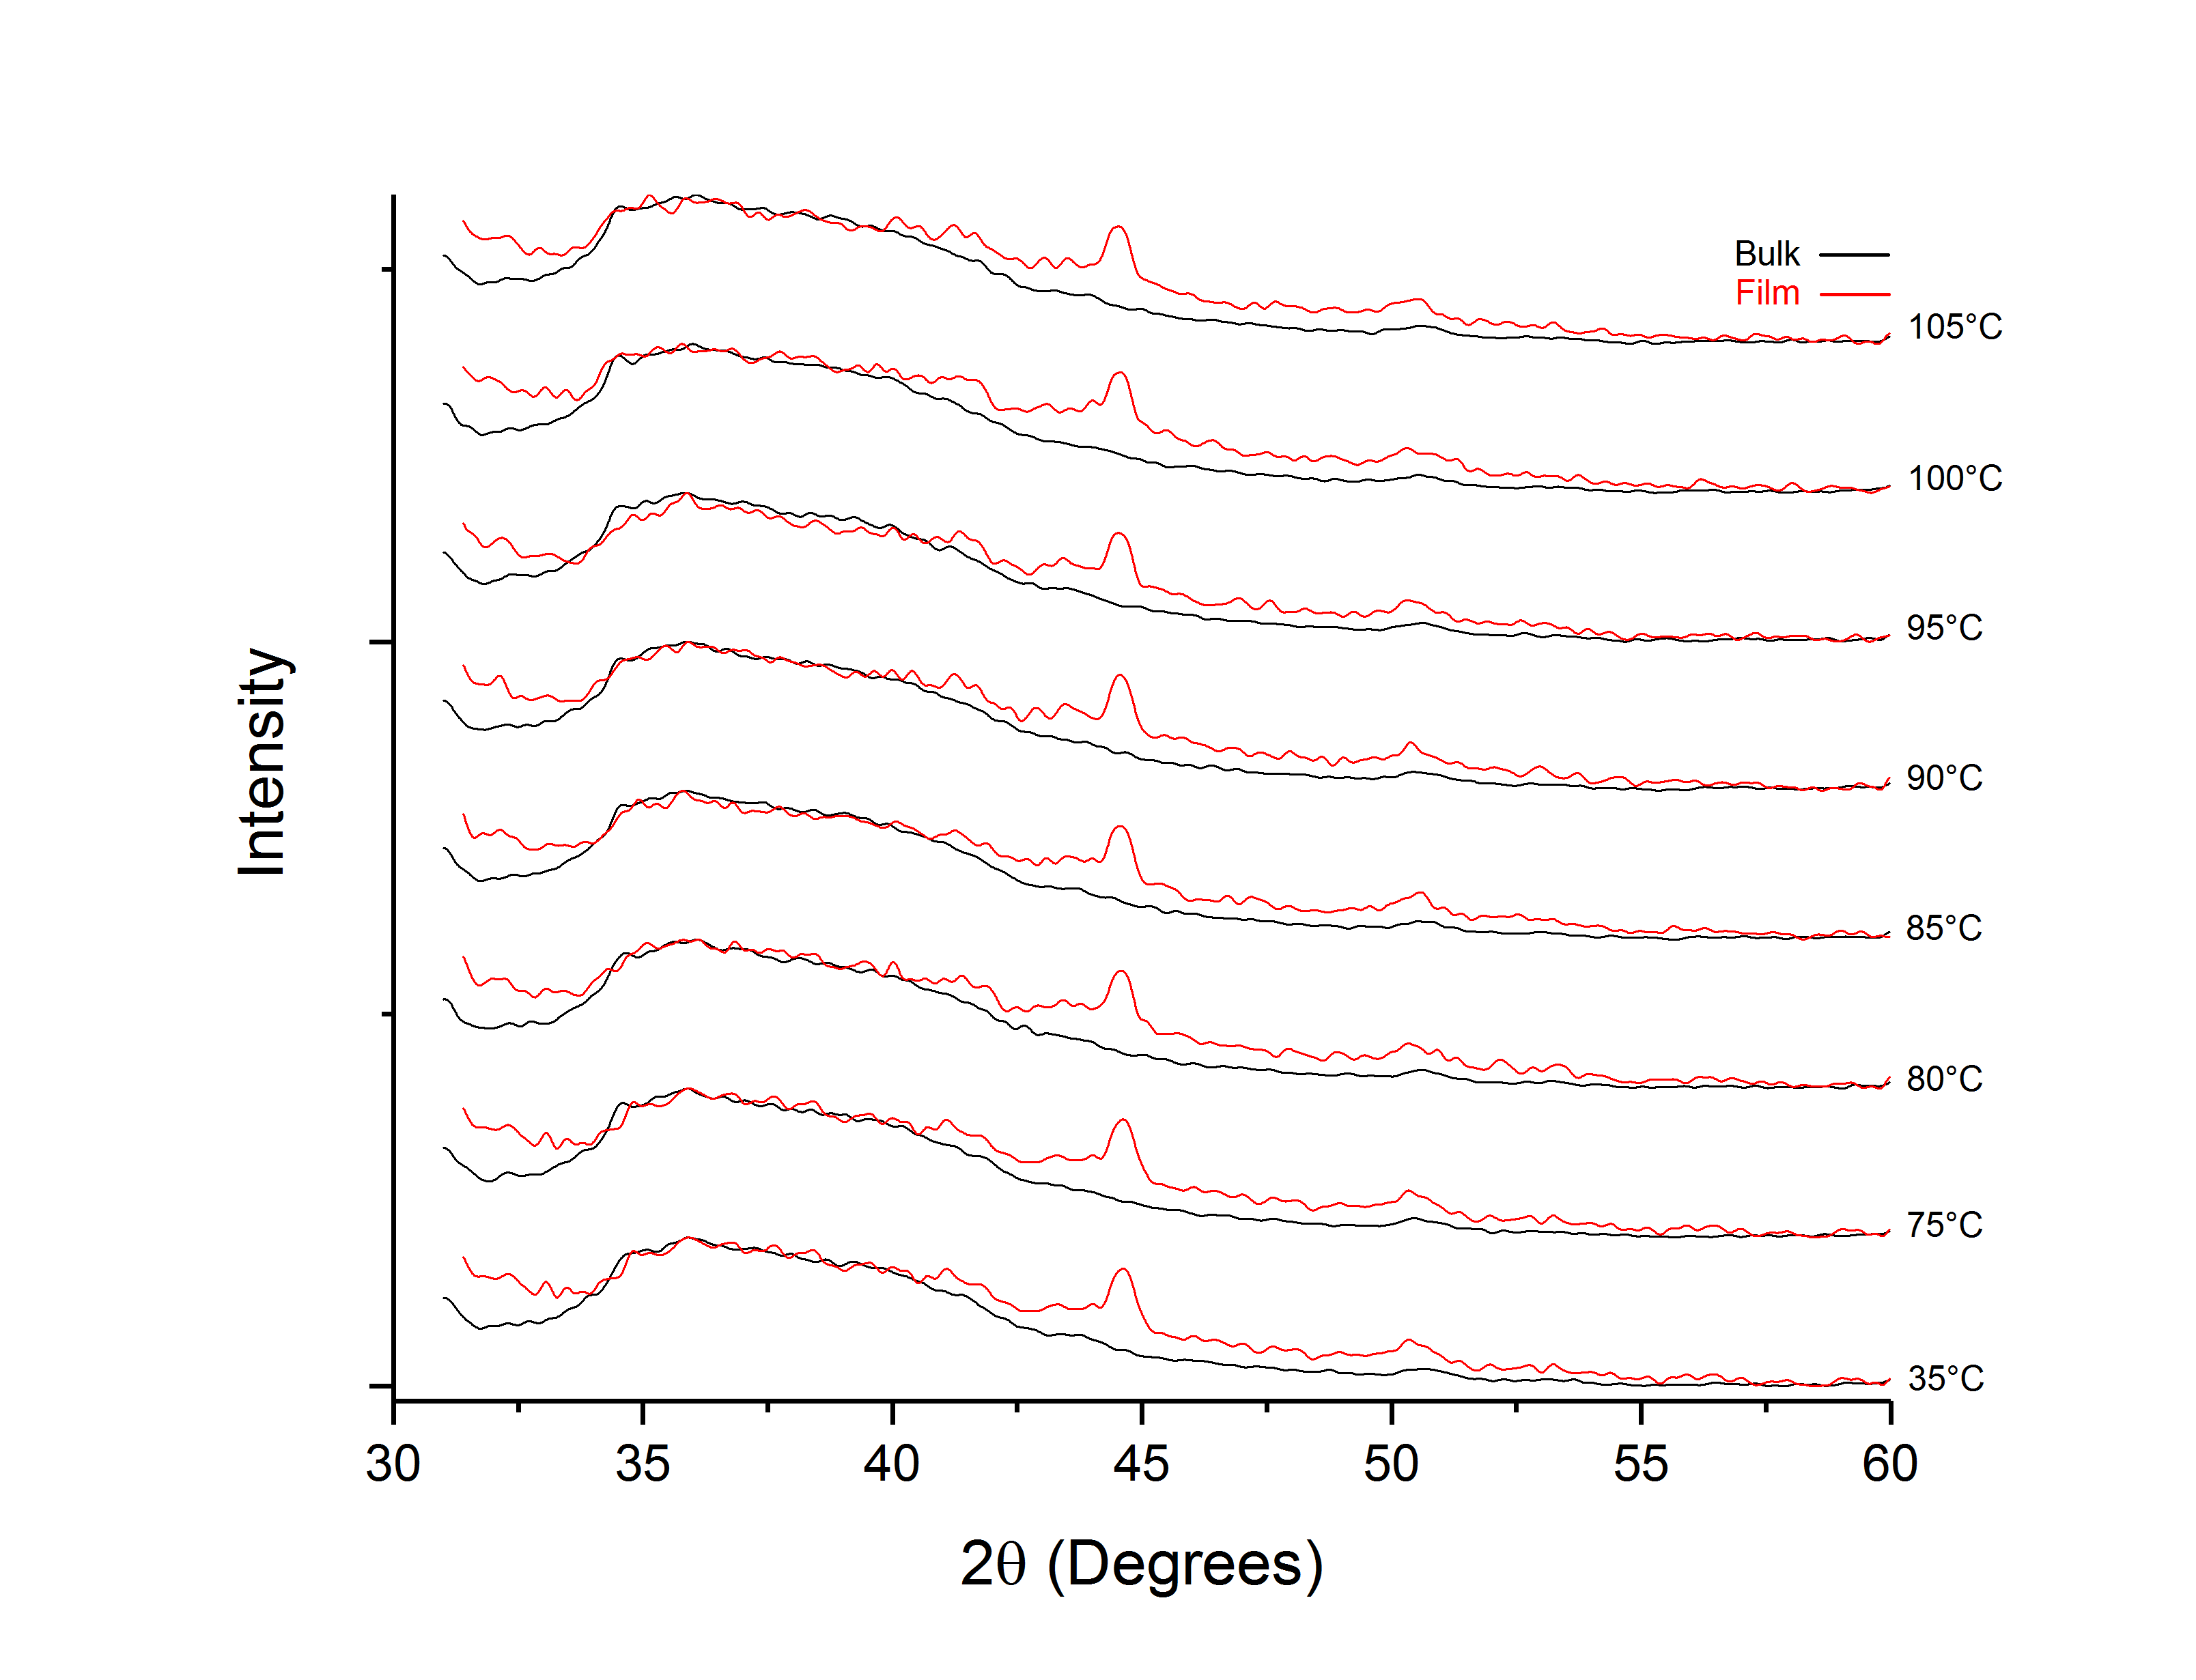
\includegraphics[width=0.85\textwidth]{XRD_Normalised_Dynamic_105.png}
	\caption[Table of contents Capition]{Normalised dynamic \acrshort{xrd} from $35-105$\degree C.}%global caption
	\label{fig:XRD_Dynamic_105}
\end{figure}

%%%%%%%%%%%%%%%%%%%%%%%%%%%%%%%%%%%%%%%%%%%%%%%%%%%%%%%%%%%%%%%%%%%%%%%%%%

\section{DISCUSSION}

The use of a 60K \gls{dsc} \acrfull{ht} compared to the more commonly used 20K rate [sources] shifts peaks for the bulk \MgZnCa~ alloy about 8 - 15 degrees higher. This higher \glspl{ht} were used because crystallisation events for the films were difficult to differentiation at the lower \glspl{ht}. 
Films show little shift to high temperature peaks with increases \glspl{ht}, but large shifts with relaxation. 
Bulk show the opposite behaviour, larger peaks shifts with higher \glspl{ht} and little shift with relaxation.

%%%%%%%%%%%%%%%%%%%%%%%%%%%%%%%%%%%%%%%%%%%%%%%%%%%%%%%%%%%%%%%%%%%%%%%%%%

\section{CONCLUSIONS}

%%%%%%%%%%%%%%%%%%%%%%%%%%%%%%%%%%%%%%%%%%%%%%%%%%%%%%%%%%%%%%%%%%%%%%%%%%

\section{ACKNOWLEDGEMENTS}

%People
Yu Wang for his assistance with \acrshort{xrd} experimentation and Rietveld refinement. 

%%%%%%%%%%%%%%%%%%%%%%%%%%%%%%%%%%%%%%%%%%%%%%%%%%%%%%%%%%%%%%%%%%%%%%%%%%

%Bibliography
\bibliography{ThesisBib}
\bibliographystyle{unsrt}

%%%%%%%%%%%%%%%%%%%%%%%%%%%%%%%%%%%%%%%%%%%%%%%%%%%%%%%%%%%%%%%%%%%%%%%%%%

%single image
\begin{figure}[b]
	\centering
	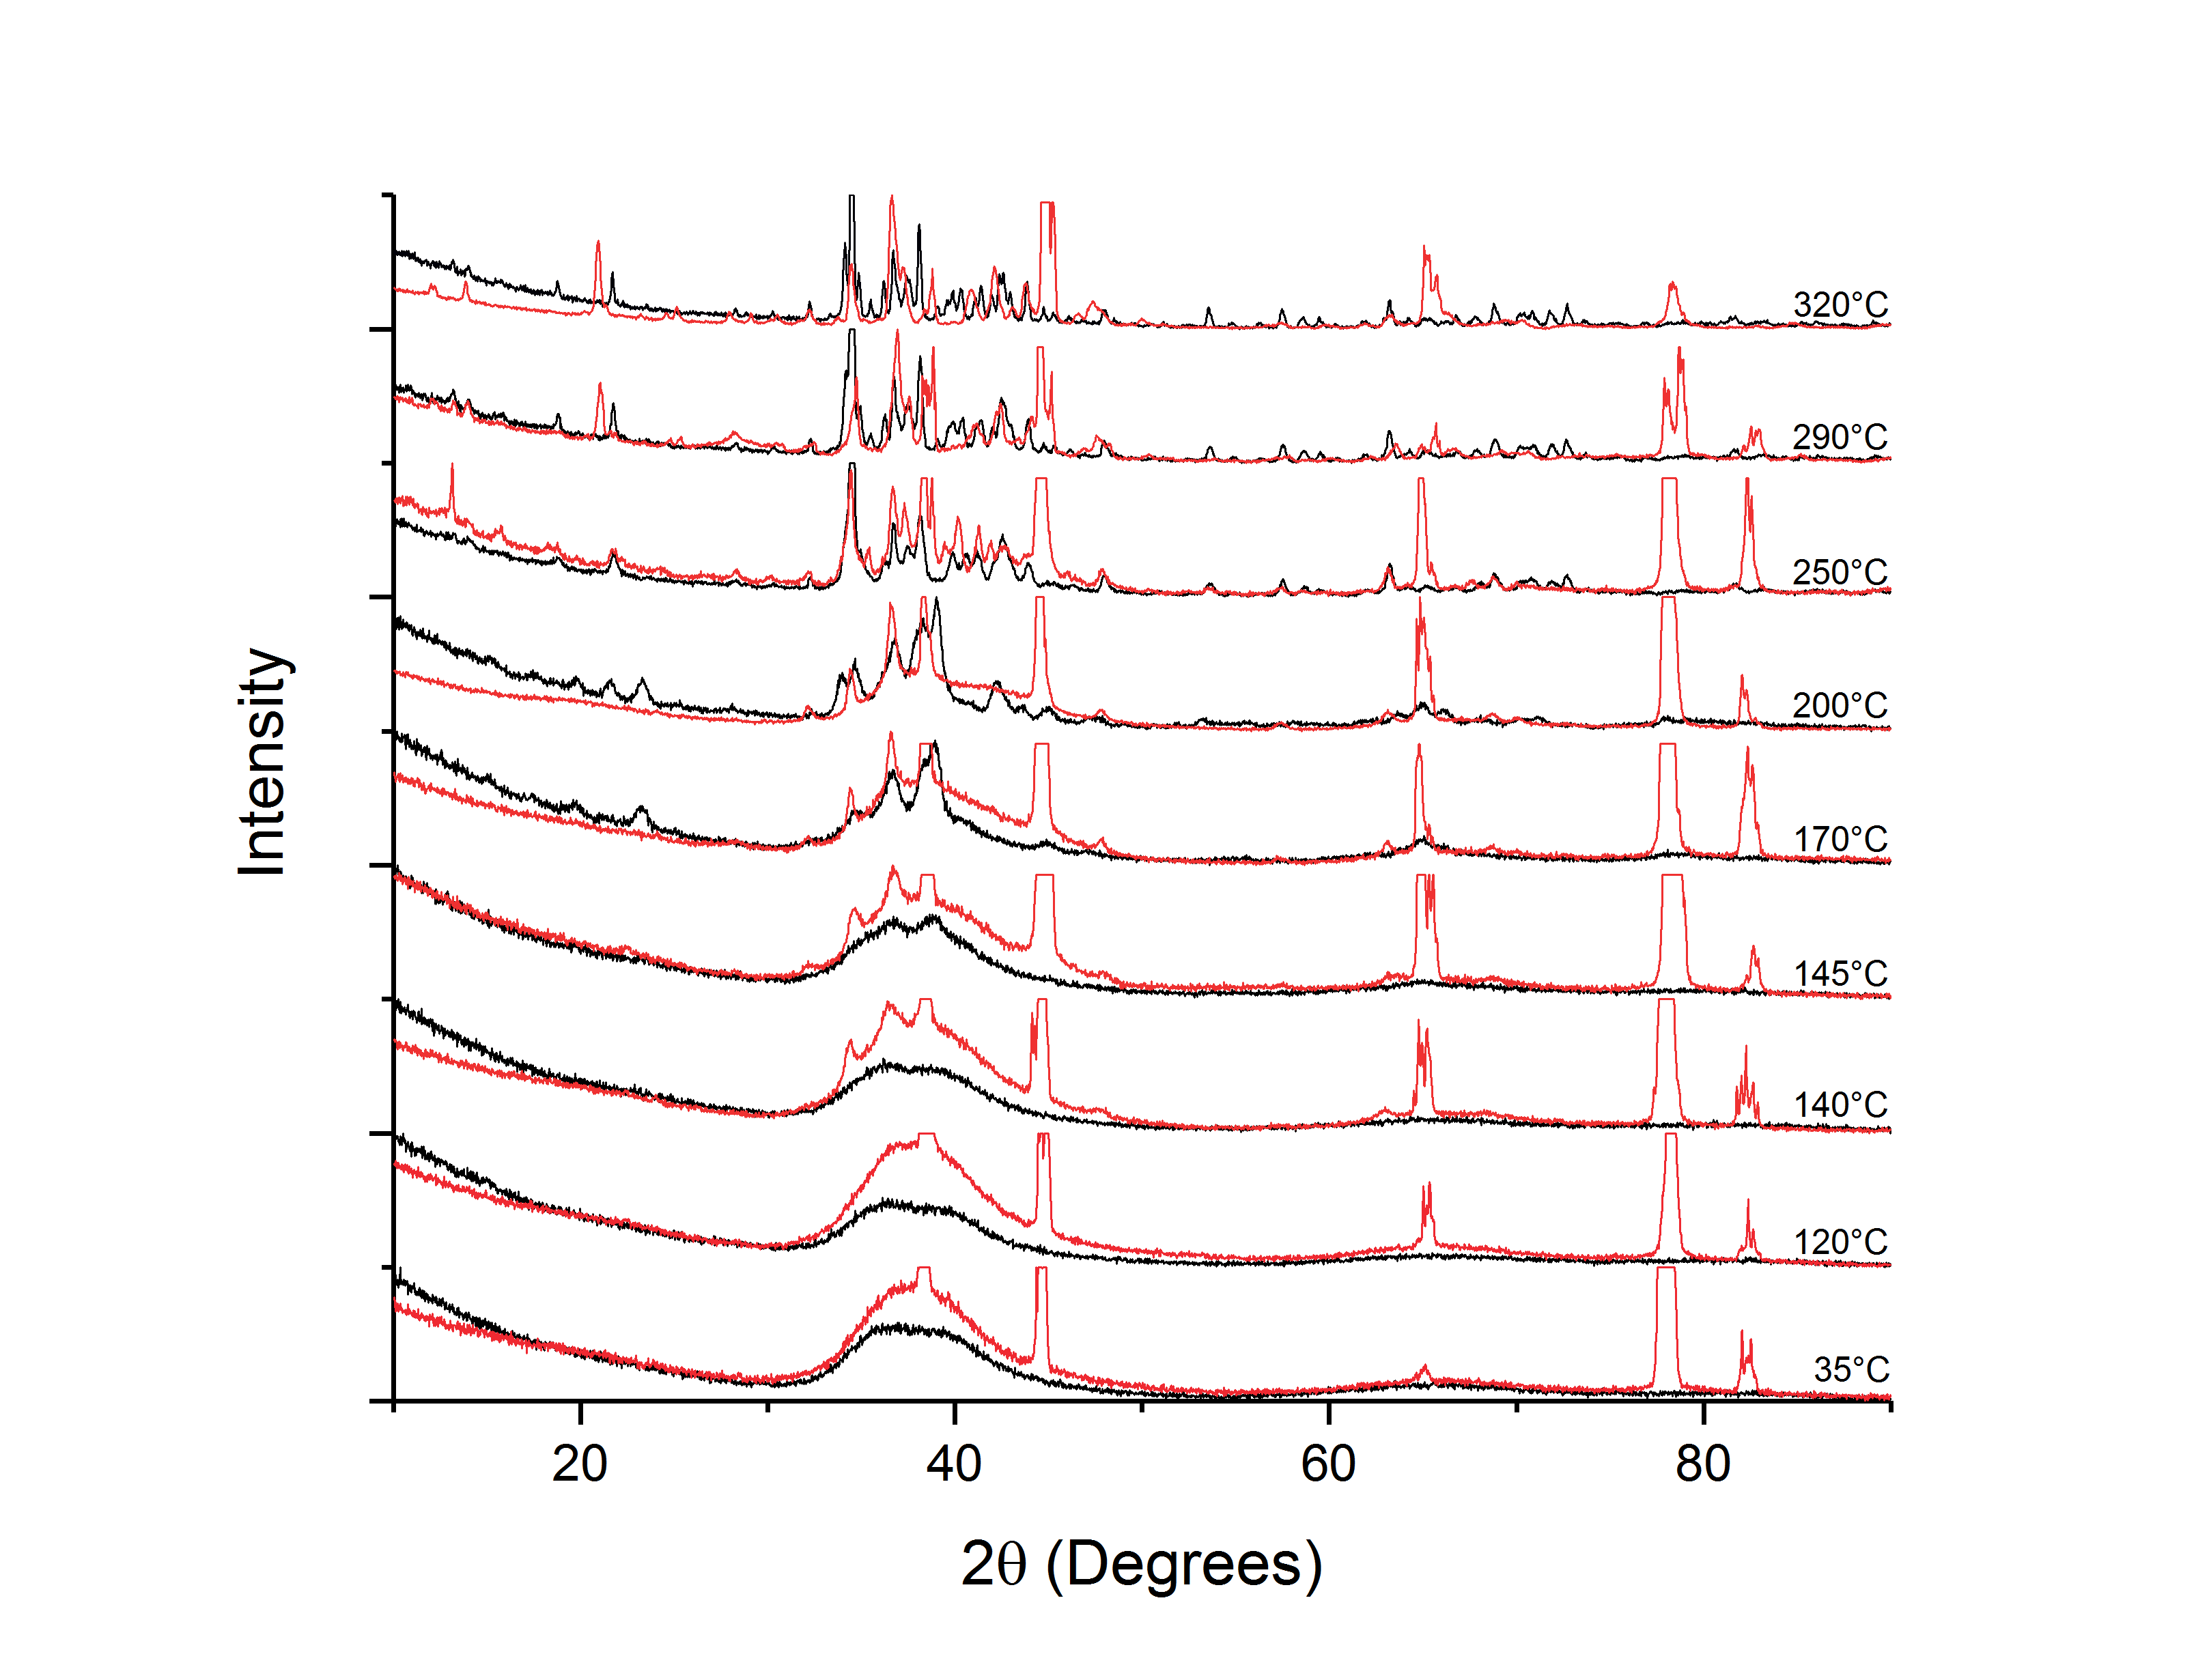
\includegraphics[width=0.99\textwidth]{XRD_Normalised_Annealing_BulkFilm_Facet.png}
	\caption{Supplementary: Normalised annealing \acrshort{xrd} pattern for both bulk and film \MgZnCa~ heated treated to several temperatures for crystallisation peak identified from \acrshort{dsc}. Bulk is shown in black, and film in red. Note the Al substrate and other high intensity peaks have been faceted as to not dwarf all other peaks.}
	\label{fig:XRD_Annealing_BulkandFilm}
\end{figure}

%single image
\begin{figure}[b]
	\centering
	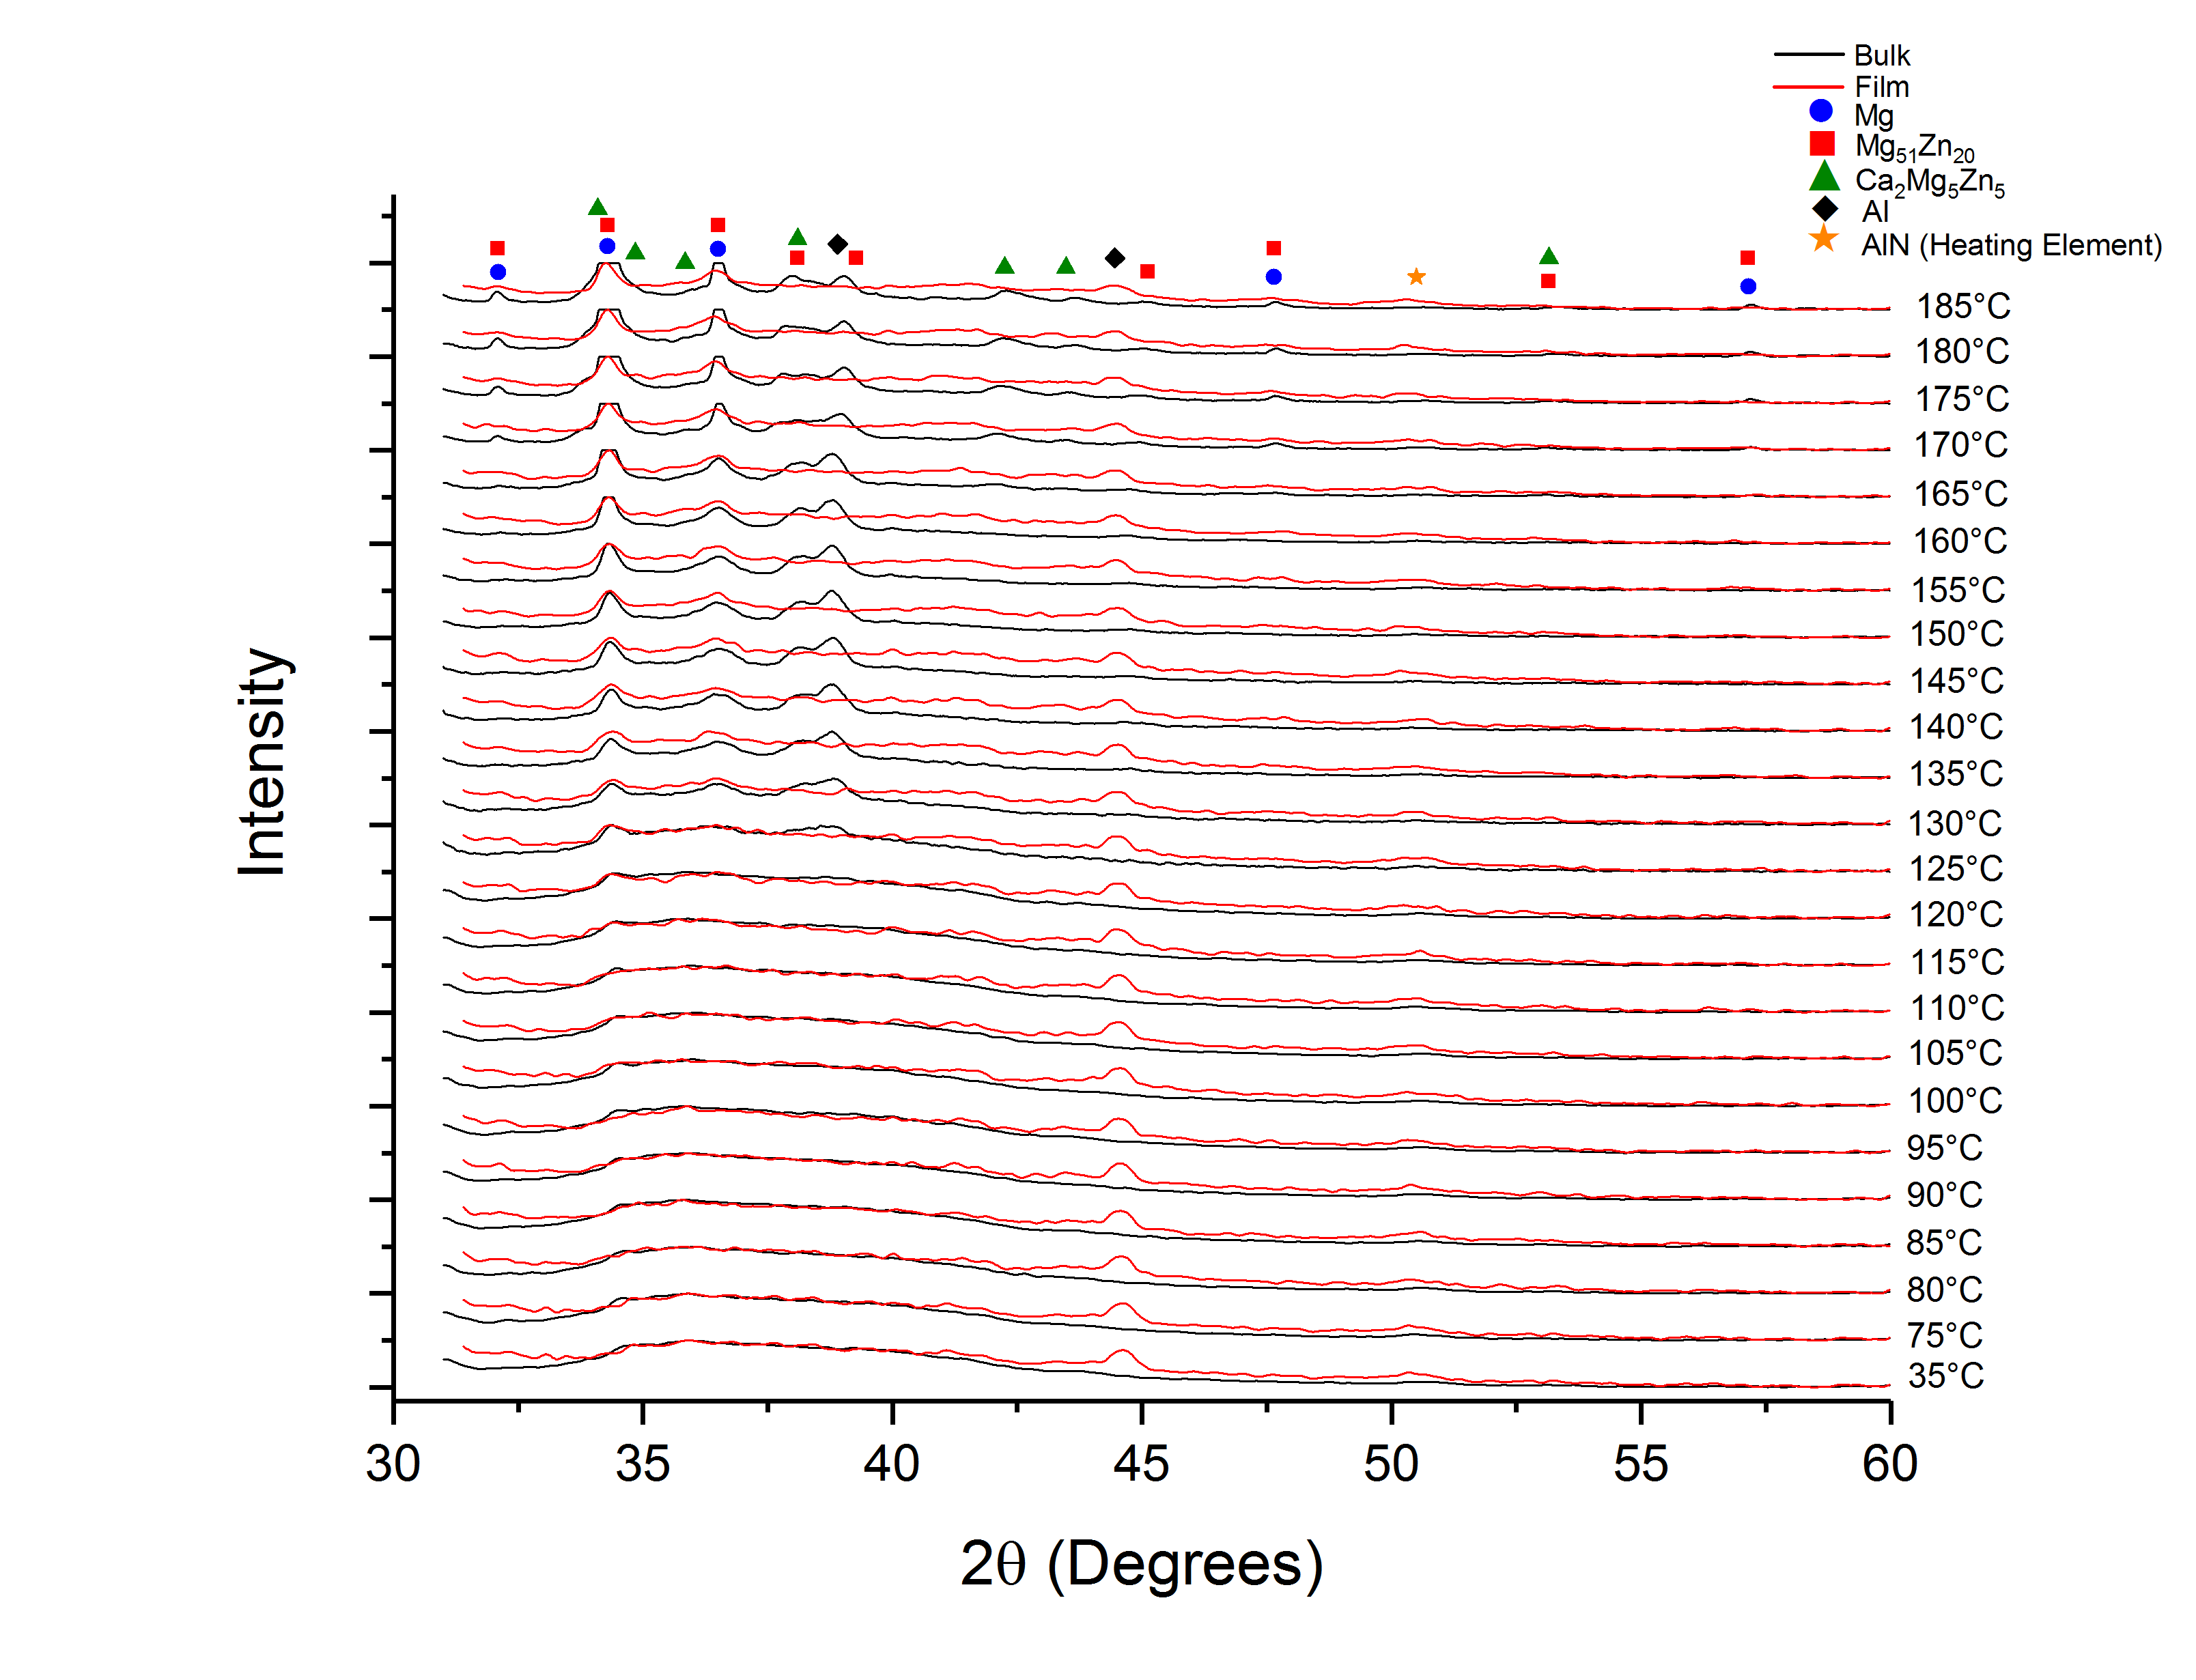
\includegraphics[width=0.99\textwidth]{XRD_Normalised_Dynamic_BulkFilm_Facet.png}
	\caption{Supplementary: Normalised dynamic \acrshort{xrd} pattern for both bulk and film \MgZnCa~ heated incrementally \textit{in-situ} from $35-185$\degree C for crystallisation peak identified from \acrshort{dsc}. Bulk is shown in black, and film in red. Note the Al substrate and other high intensity peaks have been faceted as to not dwarf all other peaks.}
	\label{fig:XRD_Dynamic_BulkandFilm}
\end{figure}

\end{document}